\documentclass[a4paper]{report}
\usepackage{answers}
\Newassociation{sol}{Solution}{ansGlobal}
\usepackage{graphics,color,eurosym,latexsym}
\usepackage{algorithm,algorithmic}
\usepackage{times, verbatim}
\newcommand{\cm}{C_{\rm m}}
\newcommand{\ty}{\texttt}
\newcommand{\sa}{\mathrm{sa}}
\newcommand{\lcp}{\mathrm{lcp}}
\newcommand{\isa}{\mathrm{isa}}
\newcommand{\suf}{\mathrm{suf}}
\newcommand{\shu}{\mathrm{shu}}
\newcommand{\pop}{\mathrm{pop}}
\newcommand{\topp}{\mathrm{top}}
\newcommand{\push}{\mathrm{push}}

%%\usepackage[nodayofweek]{datetime}
\usepackage[utf8]{inputenc}
\usepackage[OT1]{fontenc}
\usepackage{pst-all}
\usepackage{noweb}
%% \def\nwendcode{\endtrivlist \endgroup} %% prevent too much whitespace
%% \let\nwdocspar=\par                    %%   at end of pages
\def\nwendcode{\endtrivlist \endgroup \vfil\penalty10\vfilneg} %% alternative for
\let\nwdocspar=\smallbreak                                     %%   preventing spurious whitespace

\usepackage{psfrag}
\usepackage{inconsolata}
\bibliographystyle{plain}

\begin{document}
\pagestyle{noweb}

\title{\texttt{biobox}: Tools for Molecular Biology\\
\small\texttt{github.com/evolbioinf/biobox}}
\author{Bernhard Haubold}
\maketitle
\tableofcontents

\chapter{Program \texttt{al}: Align Sequences}\label{ch:al}
\input{al}
\chapter{Program \texttt{blast2dot}: Convert BLAST Output to dot Code
  for Plotting}\label{ch:b2d}
\input{blast2dot}
\chapter{Program \ty{bwt}: Burrows-Wheeler Transform}\label{ch:bw}
\input{bwt}
\chapter{Program \texttt{cchar}: Count Characters}\label{ch:cch}
\nwfilename{}\nwbegindocs{0}\nwenddocs{}\nwbegindocs{1}\nwdocspar% ===> this file was generated automatically by noweave --- better not edit it
\section*{Introduction}
Our aim is to count the residues in sequences. What we in fact do, is
to count the characters in sequences, without checking whether they
are residues or not.
\section*{Implementation}
The program outline contains hooks for imports, variables, functions,
and the meat of the main function.
\nwenddocs{}\nwbegincode{2}\sublabel{NW0-3Ni8Yu-1}\nwmargintag{{\nwtagstyle{}\subpageref{NW0-3Ni8Yu-1}}}\moddef{cchar.go~{\nwtagstyle{}\subpageref{NW0-3Ni8Yu-1}}}\endmoddef\nwstartdeflinemarkup\nwenddeflinemarkup
package main

import (
          \LA{}Imports, Ch.~\ref{ch:cch}~{\nwtagstyle{}\subpageref{NW0-MBlFE-1}}\RA{}
)

\LA{}Variables, Ch.~\ref{ch:cch}~{\nwtagstyle{}\subpageref{NW0-1qf9Wr-1}}\RA{}
\LA{}Functions, Ch.~\ref{ch:cch}~{\nwtagstyle{}\subpageref{NW0-2zJtuX-1}}\RA{}
func main() \{
          \LA{}Main function, Ch.~\ref{ch:cch}~{\nwtagstyle{}\subpageref{NW0-2WrDLN-1}}\RA{}
\}
\nwnotused{cchar.go}\nwendcode{}\nwbegindocs{3}\nwdocspar
In the \texttt{main} function we first set the usage, then parse the
options set by the user, and finally the input.
\nwenddocs{}\nwbegincode{4}\sublabel{NW0-2WrDLN-1}\nwmargintag{{\nwtagstyle{}\subpageref{NW0-2WrDLN-1}}}\moddef{Main function, Ch.~\ref{ch:cch}~{\nwtagstyle{}\subpageref{NW0-2WrDLN-1}}}\endmoddef\nwstartdeflinemarkup\nwusesondefline{\\{NW0-3Ni8Yu-1}}\nwenddeflinemarkup
\LA{}Set usage, Ch.~\ref{ch:cch}~{\nwtagstyle{}\subpageref{NW0-3OBXpn-1}}\RA{}
\LA{}Parse options, Ch.~\ref{ch:cch}~{\nwtagstyle{}\subpageref{NW0-3oBPzO-1}}\RA{}
\LA{}Parse input, Ch.~\ref{ch:cch}~{\nwtagstyle{}\subpageref{NW0-2aqsG5-1}}\RA{}
\nwused{\\{NW0-3Ni8Yu-1}}\nwendcode{}\nwbegindocs{5}\nwdocspar
In addition to the usage, we describe the purpose and give an example
command.
\nwenddocs{}\nwbegincode{6}\sublabel{NW0-3OBXpn-1}\nwmargintag{{\nwtagstyle{}\subpageref{NW0-3OBXpn-1}}}\moddef{Set usage, Ch.~\ref{ch:cch}~{\nwtagstyle{}\subpageref{NW0-3OBXpn-1}}}\endmoddef\nwstartdeflinemarkup\nwusesondefline{\\{NW0-2WrDLN-1}}\nwenddeflinemarkup
u := "cchar [-h] [options] [files]"
p := "Count characters in input."
e := "cchar -s *.fasta"
clio.Usage(u, p, e)
\nwused{\\{NW0-2WrDLN-1}}\nwendcode{}\nwbegindocs{7}\nwdocspar
We import \texttt{clio}.
\nwenddocs{}\nwbegincode{8}\sublabel{NW0-MBlFE-1}\nwmargintag{{\nwtagstyle{}\subpageref{NW0-MBlFE-1}}}\moddef{Imports, Ch.~\ref{ch:cch}~{\nwtagstyle{}\subpageref{NW0-MBlFE-1}}}\endmoddef\nwstartdeflinemarkup\nwusesondefline{\\{NW0-3Ni8Yu-1}}\nwprevnextdefs{\relax}{NW0-MBlFE-2}\nwenddeflinemarkup
"github.com/evolbioinf/clio"
\nwalsodefined{\\{NW0-MBlFE-2}\\{NW0-MBlFE-3}\\{NW0-MBlFE-4}\\{NW0-MBlFE-5}\\{NW0-MBlFE-6}\\{NW0-MBlFE-7}}\nwused{\\{NW0-3Ni8Yu-1}}\nwendcode{}\nwbegindocs{9}\nwdocspar
The user can request that each sequence is counted separately,
\texttt{-s}. There is also the possibility to just print the version
and additional information about the program, \texttt{-v}.
\nwenddocs{}\nwbegincode{10}\sublabel{NW0-1qf9Wr-1}\nwmargintag{{\nwtagstyle{}\subpageref{NW0-1qf9Wr-1}}}\moddef{Variables, Ch.~\ref{ch:cch}~{\nwtagstyle{}\subpageref{NW0-1qf9Wr-1}}}\endmoddef\nwstartdeflinemarkup\nwusesondefline{\\{NW0-3Ni8Yu-1}}\nwprevnextdefs{\relax}{NW0-1qf9Wr-2}\nwenddeflinemarkup
var optS = flag.Bool("s", false, "count sequences separately")
var optV = flag.Bool("v", false, "print version & " +
          "program information")
\nwalsodefined{\\{NW0-1qf9Wr-2}}\nwused{\\{NW0-3Ni8Yu-1}}\nwendcode{}\nwbegindocs{11}\nwdocspar
This requires the \texttt{flag} package.
\nwenddocs{}\nwbegincode{12}\sublabel{NW0-MBlFE-2}\nwmargintag{{\nwtagstyle{}\subpageref{NW0-MBlFE-2}}}\moddef{Imports, Ch.~\ref{ch:cch}~{\nwtagstyle{}\subpageref{NW0-MBlFE-1}}}\plusendmoddef\nwstartdeflinemarkup\nwusesondefline{\\{NW0-3Ni8Yu-1}}\nwprevnextdefs{NW0-MBlFE-1}{NW0-MBlFE-3}\nwenddeflinemarkup
"flag"
\nwused{\\{NW0-3Ni8Yu-1}}\nwendcode{}\nwbegindocs{13}\nwdocspar
After parsing the flags, the program might just print
its version.
\nwenddocs{}\nwbegincode{14}\sublabel{NW0-3oBPzO-1}\nwmargintag{{\nwtagstyle{}\subpageref{NW0-3oBPzO-1}}}\moddef{Parse options, Ch.~\ref{ch:cch}~{\nwtagstyle{}\subpageref{NW0-3oBPzO-1}}}\endmoddef\nwstartdeflinemarkup\nwusesondefline{\\{NW0-2WrDLN-1}}\nwenddeflinemarkup
flag.Parse()
if *optV \{
          util.PrintInfo("cchar")
\}
\nwused{\\{NW0-2WrDLN-1}}\nwendcode{}\nwbegindocs{15}\nwdocspar
We import the package \texttt{util}.
\nwenddocs{}\nwbegincode{16}\sublabel{NW0-MBlFE-3}\nwmargintag{{\nwtagstyle{}\subpageref{NW0-MBlFE-3}}}\moddef{Imports, Ch.~\ref{ch:cch}~{\nwtagstyle{}\subpageref{NW0-MBlFE-1}}}\plusendmoddef\nwstartdeflinemarkup\nwusesondefline{\\{NW0-3Ni8Yu-1}}\nwprevnextdefs{NW0-MBlFE-2}{NW0-MBlFE-4}\nwenddeflinemarkup
"github.com/evolbioinf/biobox/util"
"os"
\nwused{\\{NW0-3Ni8Yu-1}}\nwendcode{}\nwbegindocs{17}\nwdocspar
The values of \texttt{version} and \texttt{date} are injected at
compile-time. Here, we just declare them.
\nwenddocs{}\nwbegincode{18}\sublabel{NW0-1qf9Wr-2}\nwmargintag{{\nwtagstyle{}\subpageref{NW0-1qf9Wr-2}}}\moddef{Variables, Ch.~\ref{ch:cch}~{\nwtagstyle{}\subpageref{NW0-1qf9Wr-1}}}\plusendmoddef\nwstartdeflinemarkup\nwusesondefline{\\{NW0-3Ni8Yu-1}}\nwprevnextdefs{NW0-1qf9Wr-1}{\relax}\nwenddeflinemarkup
var version, date string
\nwused{\\{NW0-3Ni8Yu-1}}\nwendcode{}\nwbegindocs{19}\nwdocspar
The input files are parsed using \texttt{clio.ParseFiles}, which takes
as argument a slice of file names and a function it applies to each
file. This function takes as arguments the character counts, and an
indicator as to whether or not it is dealing with the first
sequence. At the end, \texttt{write} prints the counts.  Characters
are encoded as bytes that are eight bits long. So \texttt{counts} is a
slice of $2^8=256$ long integers.
\nwenddocs{}\nwbegincode{20}\sublabel{NW0-2aqsG5-1}\nwmargintag{{\nwtagstyle{}\subpageref{NW0-2aqsG5-1}}}\moddef{Parse input, Ch.~\ref{ch:cch}~{\nwtagstyle{}\subpageref{NW0-2aqsG5-1}}}\endmoddef\nwstartdeflinemarkup\nwusesondefline{\\{NW0-2WrDLN-1}}\nwenddeflinemarkup
files := flag.Args()
counts := make([]int64, 256)
isFirstSequence := true
clio.ParseFiles(files, scan, counts, *optS, &isFirstSequence)
write(counts, *optS)
\nwused{\\{NW0-2WrDLN-1}}\nwendcode{}\nwbegindocs{21}\nwdocspar
We import \texttt{clio}.
\nwenddocs{}\nwbegincode{22}\sublabel{NW0-MBlFE-4}\nwmargintag{{\nwtagstyle{}\subpageref{NW0-MBlFE-4}}}\moddef{Imports, Ch.~\ref{ch:cch}~{\nwtagstyle{}\subpageref{NW0-MBlFE-1}}}\plusendmoddef\nwstartdeflinemarkup\nwusesondefline{\\{NW0-3Ni8Yu-1}}\nwprevnextdefs{NW0-MBlFE-3}{NW0-MBlFE-5}\nwenddeflinemarkup
"github.com/evolbioinf/clio"
\nwused{\\{NW0-3Ni8Yu-1}}\nwendcode{}\nwbegindocs{23}\nwdocspar
Before scanning a file, the arguments are retrieved. Then the data is
scanned line-wise. Each line is either a header or consists of
characters to be counted.
\nwenddocs{}\nwbegincode{24}\sublabel{NW0-2zJtuX-1}\nwmargintag{{\nwtagstyle{}\subpageref{NW0-2zJtuX-1}}}\moddef{Functions, Ch.~\ref{ch:cch}~{\nwtagstyle{}\subpageref{NW0-2zJtuX-1}}}\endmoddef\nwstartdeflinemarkup\nwusesondefline{\\{NW0-3Ni8Yu-1}}\nwprevnextdefs{\relax}{NW0-2zJtuX-2}\nwenddeflinemarkup
func scan(r io.Reader, args ...interface\{\}) \{
          \LA{}Retrieve arguments, Ch.~\ref{ch:cch}~{\nwtagstyle{}\subpageref{NW0-11786S-1}}\RA{}
          scanner := fasta.NewScanner(r)
          for scanner.ScanLine() \{
                  if scanner.IsHeader() \{
                          \LA{}Deal with header, Ch.~\ref{ch:cch}~{\nwtagstyle{}\subpageref{NW0-4BNutl-1}}\RA{}
                  \} else \{
                          count(counts, scanner.Line())
                  \}
          \}
\}
\nwalsodefined{\\{NW0-2zJtuX-2}\\{NW0-2zJtuX-3}\\{NW0-2zJtuX-4}}\nwused{\\{NW0-3Ni8Yu-1}}\nwendcode{}\nwbegindocs{25}\nwdocspar
Import \texttt{io} and \texttt{fasta}.
\nwenddocs{}\nwbegincode{26}\sublabel{NW0-MBlFE-5}\nwmargintag{{\nwtagstyle{}\subpageref{NW0-MBlFE-5}}}\moddef{Imports, Ch.~\ref{ch:cch}~{\nwtagstyle{}\subpageref{NW0-MBlFE-1}}}\plusendmoddef\nwstartdeflinemarkup\nwusesondefline{\\{NW0-3Ni8Yu-1}}\nwprevnextdefs{NW0-MBlFE-4}{NW0-MBlFE-6}\nwenddeflinemarkup
"io"
"github.com/evolbioinf/fasta"
\nwused{\\{NW0-3Ni8Yu-1}}\nwendcode{}\nwbegindocs{27}\nwdocspar
As we saw above, \texttt{args} contains two arguments: the integer
slice of counts, and the pointer to a boolean indicating whether or
not we are dealing with the first sequence. We retrieve them by type
assertions~\cite[p. 205]{don16:go}.
\nwenddocs{}\nwbegincode{28}\sublabel{NW0-11786S-1}\nwmargintag{{\nwtagstyle{}\subpageref{NW0-11786S-1}}}\moddef{Retrieve arguments, Ch.~\ref{ch:cch}~{\nwtagstyle{}\subpageref{NW0-11786S-1}}}\endmoddef\nwstartdeflinemarkup\nwusesondefline{\\{NW0-2zJtuX-1}}\nwenddeflinemarkup
counts := args[0].([]int64)
separate := args[1].(bool)
isFirstSequence := args[2].(*bool)
\nwused{\\{NW0-2zJtuX-1}}\nwendcode{}\nwbegindocs{29}\nwdocspar
The response to encountering a header depends on whether the user has
requested separate counts for each sequence. If not, we do nothing. If
yes, we print and reset counts whenever a header closes a sequence.
\nwenddocs{}\nwbegincode{30}\sublabel{NW0-4BNutl-1}\nwmargintag{{\nwtagstyle{}\subpageref{NW0-4BNutl-1}}}\moddef{Deal with header, Ch.~\ref{ch:cch}~{\nwtagstyle{}\subpageref{NW0-4BNutl-1}}}\endmoddef\nwstartdeflinemarkup\nwusesondefline{\\{NW0-2zJtuX-1}}\nwenddeflinemarkup
if separate \{
          if *isFirstSequence \{
                  *isFirstSequence = false
          \} else \{
                  write(counts, *optS)
                  reset(counts)
          \}
          fmt.Printf("%s: ", scanner.Line())
\}
\nwused{\\{NW0-2zJtuX-1}}\nwendcode{}\nwbegindocs{31}\nwdocspar
The function \texttt{write} prints the total number of characters, and
their individual counts and frequencies.
\nwenddocs{}\nwbegincode{32}\sublabel{NW0-2zJtuX-2}\nwmargintag{{\nwtagstyle{}\subpageref{NW0-2zJtuX-2}}}\moddef{Functions, Ch.~\ref{ch:cch}~{\nwtagstyle{}\subpageref{NW0-2zJtuX-1}}}\plusendmoddef\nwstartdeflinemarkup\nwusesondefline{\\{NW0-3Ni8Yu-1}}\nwprevnextdefs{NW0-2zJtuX-1}{NW0-2zJtuX-3}\nwenddeflinemarkup
func write(counts []int64, separate bool) \{
          \LA{}Print total character count, Ch.~\ref{ch:cch}~{\nwtagstyle{}\subpageref{NW0-3hSpry-1}}\RA{}
          \LA{}Print individual counts, Ch.~\ref{ch:cch}~{\nwtagstyle{}\subpageref{NW0-4Wix1x-1}}\RA{}
\}
\nwused{\\{NW0-3Ni8Yu-1}}\nwendcode{}\nwbegindocs{33}\nwdocspar
We sum the individual character counts and print them either in ``separate''
or ``total'' mode.
\nwenddocs{}\nwbegincode{34}\sublabel{NW0-3hSpry-1}\nwmargintag{{\nwtagstyle{}\subpageref{NW0-3hSpry-1}}}\moddef{Print total character count, Ch.~\ref{ch:cch}~{\nwtagstyle{}\subpageref{NW0-3hSpry-1}}}\endmoddef\nwstartdeflinemarkup\nwusesondefline{\\{NW0-2zJtuX-2}}\nwenddeflinemarkup
var s int64
for \_, v := range counts \{
          s += v
\}
if !separate \{
          fmt.Printf("Total: ")
\}
fmt.Printf("%d\\n", s)
\nwused{\\{NW0-2zJtuX-2}}\nwendcode{}\nwbegindocs{35}\nwdocspar
We import \texttt{fmt}.
\nwenddocs{}\nwbegincode{36}\sublabel{NW0-MBlFE-6}\nwmargintag{{\nwtagstyle{}\subpageref{NW0-MBlFE-6}}}\moddef{Imports, Ch.~\ref{ch:cch}~{\nwtagstyle{}\subpageref{NW0-MBlFE-1}}}\plusendmoddef\nwstartdeflinemarkup\nwusesondefline{\\{NW0-3Ni8Yu-1}}\nwprevnextdefs{NW0-MBlFE-5}{NW0-MBlFE-7}\nwenddeflinemarkup
"fmt"
\nwused{\\{NW0-3Ni8Yu-1}}\nwendcode{}\nwbegindocs{37}\nwdocspar
If any characters were found, we print the individual counts and
frequencies in a table formatted using a \texttt{tabwriter}.
\nwenddocs{}\nwbegincode{38}\sublabel{NW0-4Wix1x-1}\nwmargintag{{\nwtagstyle{}\subpageref{NW0-4Wix1x-1}}}\moddef{Print individual counts, Ch.~\ref{ch:cch}~{\nwtagstyle{}\subpageref{NW0-4Wix1x-1}}}\endmoddef\nwstartdeflinemarkup\nwusesondefline{\\{NW0-2zJtuX-2}}\nwenddeflinemarkup
w := new(tabwriter.Writer)
w.Init(os.Stdout, 4, 0, 1, ' ', 0)
if s > 0 \{
          fmt.Fprintf(w, "Character\\tCount\\tFraction\\t\\n")
\}
for i, v := range counts \{
          if v > 0 \{
                  fmt.Fprintf(w, "%c\\t%d\\t%g\\t\\n", i, v,
                          float64(v)/float64(s))
          \}
\}
w.Flush()
\nwused{\\{NW0-2zJtuX-2}}\nwendcode{}\nwbegindocs{39}\nwdocspar
Import the \texttt{tabwriter} package.
\nwenddocs{}\nwbegincode{40}\sublabel{NW0-MBlFE-7}\nwmargintag{{\nwtagstyle{}\subpageref{NW0-MBlFE-7}}}\moddef{Imports, Ch.~\ref{ch:cch}~{\nwtagstyle{}\subpageref{NW0-MBlFE-1}}}\plusendmoddef\nwstartdeflinemarkup\nwusesondefline{\\{NW0-3Ni8Yu-1}}\nwprevnextdefs{NW0-MBlFE-6}{\relax}\nwenddeflinemarkup
"text/tabwriter"
\nwused{\\{NW0-3Ni8Yu-1}}\nwendcode{}\nwbegindocs{41}\nwdocspar
We reset the \texttt{counts}.
\nwenddocs{}\nwbegincode{42}\sublabel{NW0-2zJtuX-3}\nwmargintag{{\nwtagstyle{}\subpageref{NW0-2zJtuX-3}}}\moddef{Functions, Ch.~\ref{ch:cch}~{\nwtagstyle{}\subpageref{NW0-2zJtuX-1}}}\plusendmoddef\nwstartdeflinemarkup\nwusesondefline{\\{NW0-3Ni8Yu-1}}\nwprevnextdefs{NW0-2zJtuX-2}{NW0-2zJtuX-4}\nwenddeflinemarkup
func reset(counts []int64) \{
          for i, \_ := range counts \{
                  counts[i] = 0
          \}
\}
\nwused{\\{NW0-3Ni8Yu-1}}\nwendcode{}\nwbegindocs{43}\nwdocspar
When we at last count the characters, they serve as indexes into the
integer slice \texttt{counts}.
\nwenddocs{}\nwbegincode{44}\sublabel{NW0-2zJtuX-4}\nwmargintag{{\nwtagstyle{}\subpageref{NW0-2zJtuX-4}}}\moddef{Functions, Ch.~\ref{ch:cch}~{\nwtagstyle{}\subpageref{NW0-2zJtuX-1}}}\plusendmoddef\nwstartdeflinemarkup\nwusesondefline{\\{NW0-3Ni8Yu-1}}\nwprevnextdefs{NW0-2zJtuX-3}{\relax}\nwenddeflinemarkup
func count(counts []int64, data []byte) \{
          for \_, c := range data \{
                  counts[c]++
          \}
\}
\nwused{\\{NW0-3Ni8Yu-1}}\nwendcode{}\nwbegindocs{45}\nwdocspar
\section*{Testing}
We use the standard testing framework.
\nwenddocs{}\nwbegincode{46}\sublabel{NW0-2znUat-1}\nwmargintag{{\nwtagstyle{}\subpageref{NW0-2znUat-1}}}\moddef{cchar\_test.go~{\nwtagstyle{}\subpageref{NW0-2znUat-1}}}\endmoddef\nwstartdeflinemarkup\nwenddeflinemarkup
package main
import (
          "testing"
          \LA{}Testing imports, Ch.~\ref{ch:cch}~{\nwtagstyle{}\subpageref{NW0-4Ni3SM-1}}\RA{}
)
func TestCchar(t *testing.T) \{
          \LA{}Testing, Ch.~\ref{ch:cch}~{\nwtagstyle{}\subpageref{NW0-t5Any-1}}\RA{}
\}
\nwnotused{cchar\_test.go}\nwendcode{}\nwbegindocs{47}\nwdocspar
Our test is carried out on the file \texttt{test.fasta}, which
contains two random sequences, each 100 nucleotides long. We first run
\texttt{cchar} with default options and compare the result with that
contained in the file \texttt{res1.txt}.
\nwenddocs{}\nwbegincode{48}\sublabel{NW0-t5Any-1}\nwmargintag{{\nwtagstyle{}\subpageref{NW0-t5Any-1}}}\moddef{Testing, Ch.~\ref{ch:cch}~{\nwtagstyle{}\subpageref{NW0-t5Any-1}}}\endmoddef\nwstartdeflinemarkup\nwusesondefline{\\{NW0-2znUat-1}}\nwprevnextdefs{\relax}{NW0-t5Any-2}\nwenddeflinemarkup
cmd := exec.Command("cchar", "test.fasta")
o, err := cmd.Output()
if err != nil \{
          t.Errorf("couldn't run %q\\n", cmd)
\}
e, err := ioutil.ReadFile("res1.txt")
if err != nil \{
          t.Error("couldn't open res1.txt")
\}
if !bytes.Equal(o, e) \{
          t.Errorf("wanted:\\n%s\\ngot:\\n%s\\n", string(e), string(o))
\}
\nwalsodefined{\\{NW0-t5Any-2}}\nwused{\\{NW0-2znUat-1}}\nwendcode{}\nwbegindocs{49}\nwdocspar
We import \texttt{exec}, \texttt{ioutil}, and \texttt{bytes}.
\nwenddocs{}\nwbegincode{50}\sublabel{NW0-4Ni3SM-1}\nwmargintag{{\nwtagstyle{}\subpageref{NW0-4Ni3SM-1}}}\moddef{Testing imports, Ch.~\ref{ch:cch}~{\nwtagstyle{}\subpageref{NW0-4Ni3SM-1}}}\endmoddef\nwstartdeflinemarkup\nwusesondefline{\\{NW0-2znUat-1}}\nwenddeflinemarkup
"os/exec"
"io/ioutil"
"bytes"
\nwused{\\{NW0-2znUat-1}}\nwendcode{}\nwbegindocs{51}\nwdocspar
There is only one option to test, \texttt{-s} for counting sequences
separately. This time, we compare the result to that contained in the
file \texttt{res2.txt}.
\nwenddocs{}\nwbegincode{52}\sublabel{NW0-t5Any-2}\nwmargintag{{\nwtagstyle{}\subpageref{NW0-t5Any-2}}}\moddef{Testing, Ch.~\ref{ch:cch}~{\nwtagstyle{}\subpageref{NW0-t5Any-1}}}\plusendmoddef\nwstartdeflinemarkup\nwusesondefline{\\{NW0-2znUat-1}}\nwprevnextdefs{NW0-t5Any-1}{\relax}\nwenddeflinemarkup
cmd = exec.Command("cchar", "-s", "test.fasta")
o, err = cmd.Output()
if err != nil \{
          t.Errorf("couldn't run %q\\n", cmd)
\}
e, err = ioutil.ReadFile("res2.txt")
if err != nil \{
          t.Error("couldn't open res2.txt")
\}
if !bytes.Equal(o, e) \{
          t.Errorf("wanted:\\n%s\\ngot:\\n%s\\n", string(e), string(o))
\}
\nwused{\\{NW0-2znUat-1}}\nwendcode{}

\nwixlogsorted{c}{{cchar.go}{NW0-3Ni8Yu-1}{\nwixd{NW0-3Ni8Yu-1}}}%
\nwixlogsorted{c}{{cchar\_test.go}{NW0-2znUat-1}{\nwixd{NW0-2znUat-1}}}%
\nwixlogsorted{c}{{Deal with header, Ch.~\ref{ch:cch}}{NW0-4BNutl-1}{\nwixu{NW0-2zJtuX-1}\nwixd{NW0-4BNutl-1}}}%
\nwixlogsorted{c}{{Functions, Ch.~\ref{ch:cch}}{NW0-2zJtuX-1}{\nwixu{NW0-3Ni8Yu-1}\nwixd{NW0-2zJtuX-1}\nwixd{NW0-2zJtuX-2}\nwixd{NW0-2zJtuX-3}\nwixd{NW0-2zJtuX-4}}}%
\nwixlogsorted{c}{{Imports, Ch.~\ref{ch:cch}}{NW0-MBlFE-1}{\nwixu{NW0-3Ni8Yu-1}\nwixd{NW0-MBlFE-1}\nwixd{NW0-MBlFE-2}\nwixd{NW0-MBlFE-3}\nwixd{NW0-MBlFE-4}\nwixd{NW0-MBlFE-5}\nwixd{NW0-MBlFE-6}\nwixd{NW0-MBlFE-7}}}%
\nwixlogsorted{c}{{Main function, Ch.~\ref{ch:cch}}{NW0-2WrDLN-1}{\nwixu{NW0-3Ni8Yu-1}\nwixd{NW0-2WrDLN-1}}}%
\nwixlogsorted{c}{{Parse input, Ch.~\ref{ch:cch}}{NW0-2aqsG5-1}{\nwixu{NW0-2WrDLN-1}\nwixd{NW0-2aqsG5-1}}}%
\nwixlogsorted{c}{{Parse options, Ch.~\ref{ch:cch}}{NW0-3oBPzO-1}{\nwixu{NW0-2WrDLN-1}\nwixd{NW0-3oBPzO-1}}}%
\nwixlogsorted{c}{{Print individual counts, Ch.~\ref{ch:cch}}{NW0-4Wix1x-1}{\nwixu{NW0-2zJtuX-2}\nwixd{NW0-4Wix1x-1}}}%
\nwixlogsorted{c}{{Print total character count, Ch.~\ref{ch:cch}}{NW0-3hSpry-1}{\nwixu{NW0-2zJtuX-2}\nwixd{NW0-3hSpry-1}}}%
\nwixlogsorted{c}{{Retrieve arguments, Ch.~\ref{ch:cch}}{NW0-11786S-1}{\nwixu{NW0-2zJtuX-1}\nwixd{NW0-11786S-1}}}%
\nwixlogsorted{c}{{Set usage, Ch.~\ref{ch:cch}}{NW0-3OBXpn-1}{\nwixu{NW0-2WrDLN-1}\nwixd{NW0-3OBXpn-1}}}%
\nwixlogsorted{c}{{Testing imports, Ch.~\ref{ch:cch}}{NW0-4Ni3SM-1}{\nwixu{NW0-2znUat-1}\nwixd{NW0-4Ni3SM-1}}}%
\nwixlogsorted{c}{{Testing, Ch.~\ref{ch:cch}}{NW0-t5Any-1}{\nwixu{NW0-2znUat-1}\nwixd{NW0-t5Any-1}\nwixd{NW0-t5Any-2}}}%
\nwixlogsorted{c}{{Variables, Ch.~\ref{ch:cch}}{NW0-1qf9Wr-1}{\nwixu{NW0-3Ni8Yu-1}\nwixd{NW0-1qf9Wr-1}\nwixd{NW0-1qf9Wr-2}}}%


\chapter{Program \texttt{cutSeq}: Cut Sequence Regions}\label{ch:cut}
\input{cutSeq}
\chapter{Program \texttt{dnaDist}: Distances between DNA Sequences}\label{ch:dna}
\input{dnaDist}
\chapter{Program \ty{drawGenes}: Convert Gene Coordinates to x/y
  Coordinates}\label{ch:dg}
\input{drawGenes}
\chapter{Program \texttt{drawKt}: Draw Keyword Tree}\label{ch:dkt}
\input{drawKt}
\chapter{Program \texttt{drawSt}: Draw Suffix Tree}\label{ch:dst}
\nwfilename{}\nwbegindocs{0}\nwenddocs{}\nwbegindocs{1}\nwdocspar% ===> this file was generated automatically by noweave --- better not edit it
\section*{Introduction}
When you read a novel, you might like to look up the pages where a
particular character is mentioned. So you leaf through the book and
scan the pages for the character's name. If it's a long novel, this
takes longer than if its a short novel. But regardless of the novel's
length, this would be easier if it had an index. Most novels don't,
but most textbooks do. To look up a word in a textbook, just find it
in its index. In other words, by using an index, searching a text
becomes independent of its length.

A suffix tree is a perfect index in the sense that any word can be
looked up in it, not just particular terms considered important by an
author. Figure~\ref{fig:stConv} shows the suffix tree of the text
\[
t=\texttt{TTAAAATAT}
\]
The program \texttt{drawSt} takes as input a FASTA-formatted sequence
and draws its suffix tree.

\begin{figure}
  \begin{center}
    \begin{tabular}{cccccccccc}
        1 & 2 & 3 & 4 & 5 & 6 & 7 & 8 & 9 & 10\\
        \ty{T} & \ty{T} & \ty{A} & \ty{A} & \ty{A} & \ty{A} & \ty{T} &
        \ty{A} & \ty{T} & \ty{\$}
    \end{tabular}
  \end{center}
  \begin{center}
    \input{stree}
  \end{center}
  \caption{Suffix tree of t=\texttt{TTAAAATAT\$}.}\label{fig:stConv}
\end{figure}

Each leaf in the suffix tree in Figure~\ref{fig:stConv} is labeled by
a number. This refers to the starting position of the suffix obtained
by concatenating the characters on the path from the root to that
leaf. For example, leaf 7 has the path label \texttt{TAT\$}, the
suffix starting at position 7. This also means the tree has as many
leaves as there are suffixes---and by the same token characters---in
$t$. The last character, $\texttt{\$}$, is a sentinel that mismatches
every ordinary character to ensure that all suffixes end in a
mismatch, and hence a leaf.  Each internal node is also labeled by a
circled number, the length of its path label, also known as the node's
depth.

As explained in Chapter~\ref{ch:rep}, suffix trees are computed by
traversing their alphabetically ordered suffixes, their suffix
array. Table~\ref{tab:sa} shows the suffix array of $t$, $\sa$. If you
read it top to bottom, you get the same list of suffixes as reading
the leaves of the suffix tree left to right. Far left is the 10,
followed by 3, then 4, and so on.

The transformation of a suffix array to a suffix tree requires an
auxiliary array of the lengths of the matching prefixes of $\suf[i]$
and $\suf[i-1]$. This array is called the longest common prefix array,
$\lcp$, and is also shown in Table~\ref{tab:sa}. For example,
$\suf[4]=\texttt{AATAT\$}$ matches $\suf[3]=\texttt{AAATAT\$}$ in the
first two nucleotides, hence $\lcp[4]=2$.

\begin{table}
  \caption{Suffix array of $t=\texttt{TTAAAATAT\$}$.}\label{tab:sa}
  \begin{center}
  \begin{tabular}{cccl}
    \hline
    $i$ & $\sa[i]$ & $\lcp[i]$ & $\suf[i]$\\\hline
    1 & 10 & -1 & \texttt{\$}\\
2 & 3 & 0 & \texttt{AAAATAT\$}\\
3 & 4 & 3 & \texttt{AAATAT\$}\\
4 & 5 & 2 & \texttt{AATAT\$}\\
5 & 8 & 1 & \texttt{AT\$}\\
6 & 6 & 2 & \texttt{ATAT\$}\\
7 & 9 & 0 & \texttt{T\$}\\
8 & 2 & 1 & \texttt{TAAAATAT\$}\\
9 & 7 & 2 & \texttt{TAT\$}\\
10 & 1 & 1 & \texttt{TTAAAATAT\$}\\
\hline

    \hline
  \end{tabular}
  \end{center}
\end{table}

A suffix tree is computed by finding the intervals in $\sa$
corresponding to its internal nodes. For example, the root corresponds
to interval $[1..10]$, the node colored in red to the interval
$[2..4]$. These intervals are augmented by their depths, $d$, to give
nodes of the form $d-[\ell..r]$. Figure~\ref{fig:stInt} shows this
interval version of the suffix tree in Figure~\ref{fig:stConv}. Its
shape is that of the suffix tree in Figre~\ref{fig:stConv} stripped of
its leaves. \texttt{DrawSt} can also draw suffix trees in the interval
style.

\begin{figure}
  \begin{center}
    \input{streeI.tex}
  \end{center}
  \caption{Suffix tree of $t=\texttt{TTAAAATAT\$}$ in interval
    notation.}\label{fig:stInt}
\end{figure}

We compute the interval tree using
Algorithm~\ref{alg:st}~\cite[p. 94]{ohl13:bio}. Nodes are written as
quartets $d, \ell, r, c$, where $d$ is the depth, $\ell$ and $r$ the
left and right interval borders, and $c$ the child. An as yet unknown
right border is $-1$, no child is $\bot$. This interval tree is then
converted to the full suffix tree.
\begin{algorithm}
  \caption{Algorithm for computing suffix
    tree~\cite[p. 94]{ohl13:bio}.}\label{alg:st}
  \begin{algorithmic}
    \REQUIRE{$\sa$} \COMMENT{suffix array}
\REQUIRE{$\lcp$} \COMMENT{-1 appended}
\REQUIRE{$n$}   \COMMENT{length of $\lcp$ array}
\ENSURE{Suffix tree in interval notation}
\STATE{$v\leftarrow \bot$}
\STATE{$\mbox{push}(0, 1, -1, \bot)$} \COMMENT{push root onto stack}
\FOR{$i\leftarrow 2$ \TO $n$}
  \STATE{$\ell\leftarrow i-1$}
  \WHILE{stack not empty \AND $\lcp[i] < \mbox{top}().d$}
    \STATE{$\mbox{top}().r\leftarrow i-1$}
    \STATE{$v\leftarrow\mbox{pop}()$}
    \STATE{$\ell\leftarrow v.\ell$}
    \IF{stack not empty \AND $\lcp[i]\le\mbox{top}().d$}
      \STATE{$\mbox{top}().\mbox{addChild}(v)$}
      \STATE{$v\leftarrow\bot$}
    \ENDIF
  \ENDWHILE
  \IF{stack not empty \AND $\lcp[i] > \mbox{top}().d$}
    \STATE{$\mbox{push}(\lcp[i],\ell,-1,v)$}
    \STATE{$v\leftarrow\bot$}
  \ENDIF
\ENDFOR

  \end{algorithmic}
\end{algorithm}

Apart from the trees in Figures~\ref{fig:stConv} and \ref{fig:stInt},
\texttt{drawSt} can also produce suffix trees in the
Newick\footnote{\texttt{evolution.genetics.washington.edu/phylip/newick\_doc.html}}
notation used for phylogenies. Figure~\ref{fig:stNwk}A shows the
Newick tree string of the. This string can be converted to a proper
tree (Figure~\ref{fig:stNwk}B. Now it isn't just the branch order that
carries meaning, but also the branch lengths, as they are proportional
to the length of the path label.
\begin{figure}
  \begin{center}
    \textbf{A}\\
    \tt
    (10:1,(((3:5,4:4,5:4):1,(8:1,6:3):1):1,(9:1,(2:7,7:2,1:9):1):1):1);
  \end{center}
  \begin{center}
    \textbf{B}\\
    \begin{pspicture}(0.000,0.000)(5.833,7.500)
\psline(5.347222,7.400000)(5.833333,7.400000)
\rput(5.590278,7.600000){1}
\rput(0.486111,0.000000){\rnode{n1}{}}\uput{4pt}[0.000000]{0.000000}(n1){10}
\rput(3.888889,0.777778){\rnode{n3}{}}\uput{4pt}[0.000000]{0.000000}(n3){3}
\rput(3.402778,1.555556){\rnode{n5}{}}\uput{4pt}[0.000000]{0.000000}(n5){4}
\rput(3.402778,2.333333){\rnode{n6}{}}\uput{4pt}[0.000000]{0.000000}(n6){5}
\rput(1.458333,1.555556){\rnode{n4}{}}
\rput(1.944444,3.111111){\rnode{n8}{}}\uput{4pt}[0.000000]{0.000000}(n8){8}
\rput(2.916667,3.888889){\rnode{n10}{}}\uput{4pt}[0.000000]{0.000000}(n10){6}
\rput(1.458333,3.500000){\rnode{n9}{}}
\rput(0.972222,2.527778){\rnode{n7}{}}
\rput(1.458333,4.666667){\rnode{n12}{}}\uput{4pt}[0.000000]{0.000000}(n12){9}
\rput(4.861111,5.444445){\rnode{n14}{}}\uput{4pt}[0.000000]{0.000000}(n14){2}
\rput(2.430556,6.222222){\rnode{n16}{}}\uput{4pt}[0.000000]{0.000000}(n16){7}
\rput(5.833333,7.000000){\rnode{n17}{}}\uput{4pt}[0.000000]{0.000000}(n17){1}
\rput(1.458333,6.222222){\rnode{n15}{}}
\rput(0.972222,5.444445){\rnode{n13}{}}
\rput(0.486111,3.986111){\rnode{n11}{}}
\rput(0.000000,1.993056){\rnode{n2}{}}
\ncangle[angleB=180,angleA=-90,armB=0]{n2}{n1}
\ncangle[angleB=180,angleA=-90,armB=0]{n4}{n3}
\ncangle[angleB=180,angleA=-90,armB=0]{n4}{n5}
\ncangle[angleB=180,angleA=90,armB=0]{n4}{n6}
\ncangle[angleB=180,angleA=-90,armB=0]{n7}{n4}
\ncangle[angleB=180,angleA=-90,armB=0]{n9}{n8}
\ncangle[angleB=180,angleA=90,armB=0]{n9}{n10}
\ncangle[angleB=180,angleA=90,armB=0]{n7}{n9}
\ncangle[angleB=180,angleA=-90,armB=0]{n11}{n7}
\ncangle[angleB=180,angleA=-90,armB=0]{n13}{n12}
\ncangle[angleB=180,angleA=-90,armB=0]{n15}{n14}
\ncangle[angleB=180,angleA=-90,armB=0]{n15}{n16}
\ncangle[angleB=180,angleA=90,armB=0]{n15}{n17}
\ncangle[angleB=180,angleA=90,armB=0]{n13}{n15}
\ncangle[angleB=180,angleA=90,armB=0]{n11}{n13}
\ncangle[angleB=180,angleA=90,armB=0]{n2}{n11}
\end{pspicture}

  \end{center}
\caption{Suffix tree drawn like a phylogeny. (\textbf{A}) Newick
  notation; (\textbf{B}) drawn as tree; the scale corresponds to one character.}\label{fig:stNwk}
\end{figure}

\section*{Implementation}
The program outline contains hooks for imports, variables, types,
methods, functions, and the logic of the main function.
\nwenddocs{}\nwbegincode{2}\sublabel{NW0-1Bt7tY-1}\nwmargintag{{\nwtagstyle{}\subpageref{NW0-1Bt7tY-1}}}\moddef{drawSt.go~{\nwtagstyle{}\subpageref{NW0-1Bt7tY-1}}}\endmoddef\nwstartdeflinemarkup\nwenddeflinemarkup
package main
import (
          \LA{}Imports, Ch.~\ref{ch:dst}~{\nwtagstyle{}\subpageref{NW0-JyyYQ-1}}\RA{}
)
\LA{}Variables, Ch.~\ref{ch:dst}~{\nwtagstyle{}\subpageref{NW0-1ssEPz-1}}\RA{}
\LA{}Types, Ch.~\ref{ch:dst}~{\nwtagstyle{}\subpageref{NW0-2NSCiL-1}}\RA{}
\LA{}Methods, Ch.~\ref{ch:dst}~{\nwtagstyle{}\subpageref{NW0-1GShJr-1}}\RA{}
\LA{}Functions, Ch.~\ref{ch:dst}~{\nwtagstyle{}\subpageref{NW0-2wzOEh-1}}\RA{}
func main() \{
          \LA{}Main function, Ch.~\ref{ch:dst}~{\nwtagstyle{}\subpageref{NW0-2Ue6PL-1}}\RA{}
\}
\nwnotused{drawSt.go}\nwendcode{}\nwbegindocs{3}\nwdocspar
In the main function we set the usage, declare and parse the options,
and parse the input files.
\nwenddocs{}\nwbegincode{4}\sublabel{NW0-2Ue6PL-1}\nwmargintag{{\nwtagstyle{}\subpageref{NW0-2Ue6PL-1}}}\moddef{Main function, Ch.~\ref{ch:dst}~{\nwtagstyle{}\subpageref{NW0-2Ue6PL-1}}}\endmoddef\nwstartdeflinemarkup\nwusesondefline{\\{NW0-1Bt7tY-1}}\nwenddeflinemarkup
\LA{}Set usage, Ch.~\ref{ch:dst}~{\nwtagstyle{}\subpageref{NW0-3QNT53-1}}\RA{}
\LA{}Declare options, Ch.~\ref{ch:dst}~{\nwtagstyle{}\subpageref{NW0-2H6NhM-1}}\RA{}
\LA{}Parse options, Ch.~\ref{ch:dst}~{\nwtagstyle{}\subpageref{NW0-3qXFXs-1}}\RA{}
\LA{}Parse input files, Ch.~\ref{ch:dst}~{\nwtagstyle{}\subpageref{NW0-4CQUp5-1}}\RA{}
\nwused{\\{NW0-1Bt7tY-1}}\nwendcode{}\nwbegindocs{5}\nwdocspar
The usage consists of three parts, the actual usage message, an
explanation of the program's purpose, and an example command.
\nwenddocs{}\nwbegincode{6}\sublabel{NW0-3QNT53-1}\nwmargintag{{\nwtagstyle{}\subpageref{NW0-3QNT53-1}}}\moddef{Set usage, Ch.~\ref{ch:dst}~{\nwtagstyle{}\subpageref{NW0-3QNT53-1}}}\endmoddef\nwstartdeflinemarkup\nwusesondefline{\\{NW0-2Ue6PL-1}}\nwenddeflinemarkup
m := "drawSt [-h] [options] [files]"
p := "Draw suffix tree."
e := "drawSt foo.fasta"
clio.Usage(m, p, e)
\nwused{\\{NW0-2Ue6PL-1}}\nwendcode{}\nwbegindocs{7}\nwdocspar
We import \texttt{clio}.
\nwenddocs{}\nwbegincode{8}\sublabel{NW0-JyyYQ-1}\nwmargintag{{\nwtagstyle{}\subpageref{NW0-JyyYQ-1}}}\moddef{Imports, Ch.~\ref{ch:dst}~{\nwtagstyle{}\subpageref{NW0-JyyYQ-1}}}\endmoddef\nwstartdeflinemarkup\nwusesondefline{\\{NW0-1Bt7tY-1}}\nwprevnextdefs{\relax}{NW0-JyyYQ-2}\nwenddeflinemarkup
"github.com/evolbioinf/clio"
\nwalsodefined{\\{NW0-JyyYQ-2}\\{NW0-JyyYQ-3}\\{NW0-JyyYQ-4}\\{NW0-JyyYQ-5}\\{NW0-JyyYQ-6}\\{NW0-JyyYQ-7}\\{NW0-JyyYQ-8}}\nwused{\\{NW0-1Bt7tY-1}}\nwendcode{}\nwbegindocs{9}\nwdocspar
By default, the program specifies the tree in \LaTeX{} using the
conventional notation of Figure~\ref{fig:stConv}. We declare options
for the two alternative formats, interval notation (\ty{-i},
Figure~\ref{fig:stInt}), and Newick notation (\ty{-n},
Figure~\ref{fig:stNwk}A). The user can also print the node depth
(\ty{-d}), label the nodes (\ty{-l}), change the default x- and
y-units (\ty{-x} \& \ty{-y}), add a sentinel character, and print the
program version (\ty{-v}).
\nwenddocs{}\nwbegincode{10}\sublabel{NW0-2H6NhM-1}\nwmargintag{{\nwtagstyle{}\subpageref{NW0-2H6NhM-1}}}\moddef{Declare options, Ch.~\ref{ch:dst}~{\nwtagstyle{}\subpageref{NW0-2H6NhM-1}}}\endmoddef\nwstartdeflinemarkup\nwusesondefline{\\{NW0-2Ue6PL-1}}\nwenddeflinemarkup
var optI = flag.Bool("i", false, "interval notation, LaTeX")
var optN = flag.Bool("n", false, "Newick notation, plain text")
var optD = flag.Bool("d", false, "show node depth")
var optL = flag.Bool("l", false, "label nodes")
var optX = flag.Float64("x", 1, "x-unit in LaTeX")
var optY = flag.Float64("y", 1.5, "y-unit in LaTeX")
var optS = flag.Bool("s", false, "add sentinel character")
var optV = flag.Bool("v", false, "print program version & " +
          "other information")
\nwused{\\{NW0-2Ue6PL-1}}\nwendcode{}\nwbegindocs{11}\nwdocspar
We import \texttt{flag}.
\nwenddocs{}\nwbegincode{12}\sublabel{NW0-JyyYQ-2}\nwmargintag{{\nwtagstyle{}\subpageref{NW0-JyyYQ-2}}}\moddef{Imports, Ch.~\ref{ch:dst}~{\nwtagstyle{}\subpageref{NW0-JyyYQ-1}}}\plusendmoddef\nwstartdeflinemarkup\nwusesondefline{\\{NW0-1Bt7tY-1}}\nwprevnextdefs{NW0-JyyYQ-1}{NW0-JyyYQ-3}\nwenddeflinemarkup
"flag"
\nwused{\\{NW0-1Bt7tY-1}}\nwendcode{}\nwbegindocs{13}\nwdocspar
We parse the options and respond to \ty{-v}.
\nwenddocs{}\nwbegincode{14}\sublabel{NW0-3qXFXs-1}\nwmargintag{{\nwtagstyle{}\subpageref{NW0-3qXFXs-1}}}\moddef{Parse options, Ch.~\ref{ch:dst}~{\nwtagstyle{}\subpageref{NW0-3qXFXs-1}}}\endmoddef\nwstartdeflinemarkup\nwusesondefline{\\{NW0-2Ue6PL-1}}\nwenddeflinemarkup
flag.Parse()
if *optV \{
          util.PrintInfo("drawSt")
\}
\nwused{\\{NW0-2Ue6PL-1}}\nwendcode{}\nwbegindocs{15}\nwdocspar
We import \texttt{util}.
\nwenddocs{}\nwbegincode{16}\sublabel{NW0-JyyYQ-3}\nwmargintag{{\nwtagstyle{}\subpageref{NW0-JyyYQ-3}}}\moddef{Imports, Ch.~\ref{ch:dst}~{\nwtagstyle{}\subpageref{NW0-JyyYQ-1}}}\plusendmoddef\nwstartdeflinemarkup\nwusesondefline{\\{NW0-1Bt7tY-1}}\nwprevnextdefs{NW0-JyyYQ-2}{NW0-JyyYQ-4}\nwenddeflinemarkup
"github.com/evolbioinf/biobox/util"
\nwused{\\{NW0-1Bt7tY-1}}\nwendcode{}\nwbegindocs{17}\nwdocspar
The remaining tokens on the command line are interpreted as input
files, which get parsed using the function \ty{scan}. It takes as
arguments the seven options specifying the tree format.
\nwenddocs{}\nwbegincode{18}\sublabel{NW0-4CQUp5-1}\nwmargintag{{\nwtagstyle{}\subpageref{NW0-4CQUp5-1}}}\moddef{Parse input files, Ch.~\ref{ch:dst}~{\nwtagstyle{}\subpageref{NW0-4CQUp5-1}}}\endmoddef\nwstartdeflinemarkup\nwusesondefline{\\{NW0-2Ue6PL-1}}\nwenddeflinemarkup
files := flag.Args()
clio.ParseFiles(files, scan, *optI, *optN, *optD, *optL, *optX,
          *optY, *optS)
\nwused{\\{NW0-2Ue6PL-1}}\nwendcode{}\nwbegindocs{19}\nwdocspar
In \texttt{scan}, we retrieve the options before iterating over the
sequences in the file.
\nwenddocs{}\nwbegincode{20}\sublabel{NW0-2wzOEh-1}\nwmargintag{{\nwtagstyle{}\subpageref{NW0-2wzOEh-1}}}\moddef{Functions, Ch.~\ref{ch:dst}~{\nwtagstyle{}\subpageref{NW0-2wzOEh-1}}}\endmoddef\nwstartdeflinemarkup\nwusesondefline{\\{NW0-1Bt7tY-1}}\nwprevnextdefs{\relax}{NW0-2wzOEh-2}\nwenddeflinemarkup
func scan(r io.Reader, args ...interface\{\}) \{
          \LA{}Retrieve options, Ch.~\ref{ch:dst}~{\nwtagstyle{}\subpageref{NW0-3vLqZ0-1}}\RA{}
          \LA{}Iterate over sequences, Ch.~\ref{ch:dst}~{\nwtagstyle{}\subpageref{NW0-3YShji-1}}\RA{}
\}
\nwalsodefined{\\{NW0-2wzOEh-2}\\{NW0-2wzOEh-3}\\{NW0-2wzOEh-4}\\{NW0-2wzOEh-5}\\{NW0-2wzOEh-6}\\{NW0-2wzOEh-7}\\{NW0-2wzOEh-8}\\{NW0-2wzOEh-9}\\{NW0-2wzOEh-A}\\{NW0-2wzOEh-B}}\nwused{\\{NW0-1Bt7tY-1}}\nwendcode{}\nwbegindocs{21}\nwdocspar
We import \ty{io}.
\nwenddocs{}\nwbegincode{22}\sublabel{NW0-JyyYQ-4}\nwmargintag{{\nwtagstyle{}\subpageref{NW0-JyyYQ-4}}}\moddef{Imports, Ch.~\ref{ch:dst}~{\nwtagstyle{}\subpageref{NW0-JyyYQ-1}}}\plusendmoddef\nwstartdeflinemarkup\nwusesondefline{\\{NW0-1Bt7tY-1}}\nwprevnextdefs{NW0-JyyYQ-3}{NW0-JyyYQ-5}\nwenddeflinemarkup
"io"
\nwused{\\{NW0-1Bt7tY-1}}\nwendcode{}\nwbegindocs{23}\nwdocspar
The seven options just passed are retrieved by reflection.
\nwenddocs{}\nwbegincode{24}\sublabel{NW0-3vLqZ0-1}\nwmargintag{{\nwtagstyle{}\subpageref{NW0-3vLqZ0-1}}}\moddef{Retrieve options, Ch.~\ref{ch:dst}~{\nwtagstyle{}\subpageref{NW0-3vLqZ0-1}}}\endmoddef\nwstartdeflinemarkup\nwusesondefline{\\{NW0-2wzOEh-1}}\nwenddeflinemarkup
optI := args[0].(bool)
optN := args[1].(bool)
optD := args[2].(bool)
optL := args[3].(bool)
optX := args[4].(float64)
optY := args[5].(float64)
optS := args[6].(bool)
\nwused{\\{NW0-2wzOEh-1}}\nwendcode{}\nwbegindocs{25}\nwdocspar
For each sequence, we extract the sequence data, compute the suffix
tree, and draw it.
\nwenddocs{}\nwbegincode{26}\sublabel{NW0-3YShji-1}\nwmargintag{{\nwtagstyle{}\subpageref{NW0-3YShji-1}}}\moddef{Iterate over sequences, Ch.~\ref{ch:dst}~{\nwtagstyle{}\subpageref{NW0-3YShji-1}}}\endmoddef\nwstartdeflinemarkup\nwusesondefline{\\{NW0-2wzOEh-1}}\nwenddeflinemarkup
scanner := fasta.NewScanner(r)
for scanner.ScanSequence() \{
          sequence := scanner.Sequence()
          data := sequence.Data()
          \LA{}Compute suffix tree, Ch.~\ref{ch:dst}~{\nwtagstyle{}\subpageref{NW0-3rgVLJ-1}}\RA{}
          \LA{}Draw suffix tree, Ch.~\ref{ch:dst}~{\nwtagstyle{}\subpageref{NW0-2DUupi-1}}\RA{}
\}
\nwused{\\{NW0-2wzOEh-1}}\nwendcode{}\nwbegindocs{27}\nwdocspar
We import \ty{fasta}.
\nwenddocs{}\nwbegincode{28}\sublabel{NW0-JyyYQ-5}\nwmargintag{{\nwtagstyle{}\subpageref{NW0-JyyYQ-5}}}\moddef{Imports, Ch.~\ref{ch:dst}~{\nwtagstyle{}\subpageref{NW0-JyyYQ-1}}}\plusendmoddef\nwstartdeflinemarkup\nwusesondefline{\\{NW0-1Bt7tY-1}}\nwprevnextdefs{NW0-JyyYQ-4}{NW0-JyyYQ-6}\nwenddeflinemarkup
"github.com/evolbioinf/fasta"
\nwused{\\{NW0-1Bt7tY-1}}\nwendcode{}\nwbegindocs{29}\nwdocspar
A suffix tree consists of nodes, which in turn consist of a depth, a
left border, and a right border. The tree topology is established
through references to a child node and a sibling. In a conventional
suffix tree (Figure~\ref{fig:stConv}), each incoming edge of a node
has a label. We don't store the label but compute it whenever
required. To do that, we need to know not only the current node's
depth, but also its parent's, and hence include a pointer to parent. A
node also has an ID for easy reference and a level in the tree.
\nwenddocs{}\nwbegincode{30}\sublabel{NW0-2NSCiL-1}\nwmargintag{{\nwtagstyle{}\subpageref{NW0-2NSCiL-1}}}\moddef{Types, Ch.~\ref{ch:dst}~{\nwtagstyle{}\subpageref{NW0-2NSCiL-1}}}\endmoddef\nwstartdeflinemarkup\nwusesondefline{\\{NW0-1Bt7tY-1}}\nwprevnextdefs{\relax}{NW0-2NSCiL-2}\nwenddeflinemarkup
type node struct \{
          d, l, r, id, level int
          child, sib, parent *node
\}
\nwalsodefined{\\{NW0-2NSCiL-2}\\{NW0-2NSCiL-3}}\nwused{\\{NW0-1Bt7tY-1}}\nwendcode{}\nwbegindocs{31}\nwdocspar
For easy printing of nodes we implement \texttt{String}.
\nwenddocs{}\nwbegincode{32}\sublabel{NW0-1GShJr-1}\nwmargintag{{\nwtagstyle{}\subpageref{NW0-1GShJr-1}}}\moddef{Methods, Ch.~\ref{ch:dst}~{\nwtagstyle{}\subpageref{NW0-1GShJr-1}}}\endmoddef\nwstartdeflinemarkup\nwusesondefline{\\{NW0-1Bt7tY-1}}\nwprevnextdefs{\relax}{NW0-1GShJr-2}\nwenddeflinemarkup
func (v *node) String() string \{
          if v == nil \{
                  return "!"
          \}
          s := fmt.Sprintf("%d-[%d..%d]", v.d, v.l, v.r)
          return s
\}
\nwalsodefined{\\{NW0-1GShJr-2}\\{NW0-1GShJr-3}}\nwused{\\{NW0-1Bt7tY-1}}\nwendcode{}\nwbegindocs{33}\nwdocspar
A new node is constructed as a function of its depth, left and right
borders, and child node.
\nwenddocs{}\nwbegincode{34}\sublabel{NW0-2wzOEh-2}\nwmargintag{{\nwtagstyle{}\subpageref{NW0-2wzOEh-2}}}\moddef{Functions, Ch.~\ref{ch:dst}~{\nwtagstyle{}\subpageref{NW0-2wzOEh-1}}}\plusendmoddef\nwstartdeflinemarkup\nwusesondefline{\\{NW0-1Bt7tY-1}}\nwprevnextdefs{NW0-2wzOEh-1}{NW0-2wzOEh-3}\nwenddeflinemarkup
func newNode(d, l, r int, child *node) *node \{
          n := new(node)
          n.d = d
          n.l = l
          n.r = r
          n.id = nodeId
          nodeId++
          if child != nil \{
                  n.child = child
                  child.parent = n
          \}
          return n
\}
\nwused{\\{NW0-1Bt7tY-1}}\nwendcode{}\nwbegindocs{35}\nwdocspar
The node identifier is kept in a global variable.
\nwenddocs{}\nwbegincode{36}\sublabel{NW0-1ssEPz-1}\nwmargintag{{\nwtagstyle{}\subpageref{NW0-1ssEPz-1}}}\moddef{Variables, Ch.~\ref{ch:dst}~{\nwtagstyle{}\subpageref{NW0-1ssEPz-1}}}\endmoddef\nwstartdeflinemarkup\nwusesondefline{\\{NW0-1Bt7tY-1}}\nwenddeflinemarkup
var nodeId int
\nwused{\\{NW0-1Bt7tY-1}}\nwendcode{}\nwbegindocs{37}\nwdocspar
According to Algorithm~\ref{alg:st}, the nodes are kept on a stack,
which we implement as a slice of node pointers~\cite[p. 92]{don16:go}.
\nwenddocs{}\nwbegincode{38}\sublabel{NW0-2NSCiL-2}\nwmargintag{{\nwtagstyle{}\subpageref{NW0-2NSCiL-2}}}\moddef{Types, Ch.~\ref{ch:dst}~{\nwtagstyle{}\subpageref{NW0-2NSCiL-1}}}\plusendmoddef\nwstartdeflinemarkup\nwusesondefline{\\{NW0-1Bt7tY-1}}\nwprevnextdefs{NW0-2NSCiL-1}{NW0-2NSCiL-3}\nwenddeflinemarkup
type stack []*node
\nwused{\\{NW0-1Bt7tY-1}}\nwendcode{}\nwbegindocs{39}\nwdocspar
We implement the three canonical stack functions, push, pop, and top.
\nwenddocs{}\nwbegincode{40}\sublabel{NW0-1GShJr-2}\nwmargintag{{\nwtagstyle{}\subpageref{NW0-1GShJr-2}}}\moddef{Methods, Ch.~\ref{ch:dst}~{\nwtagstyle{}\subpageref{NW0-1GShJr-1}}}\plusendmoddef\nwstartdeflinemarkup\nwusesondefline{\\{NW0-1Bt7tY-1}}\nwprevnextdefs{NW0-1GShJr-1}{NW0-1GShJr-3}\nwenddeflinemarkup
func (s *stack) push(n *node) \{ *s = append(*s, n) \}
func (s *stack) pop() *node \{
          n := (*s)[len(*s)-1]
          *s = (*s)[0:len(*s)-1]
          return n
\}
func (s *stack) top() *node \{ return (*s)[len(*s)-1] \}
\nwused{\\{NW0-1Bt7tY-1}}\nwendcode{}\nwbegindocs{41}\nwdocspar
To compute the suffix tree, we first prepare the data. The basis for
our suffix tree is the enhanced suffix array consisting of the suffix
array proper and the lcp array. The lcp array gets a -1 appended to
ensure all nodes are eventually popped from the stack in the while
loop of Algorithm~\ref{alg:st}.  We also initialize the focal node,
$v$, and the stack, onto which we push the root. Then we traverse the
lcp array.
\nwenddocs{}\nwbegincode{42}\sublabel{NW0-3rgVLJ-1}\nwmargintag{{\nwtagstyle{}\subpageref{NW0-3rgVLJ-1}}}\moddef{Compute suffix tree, Ch.~\ref{ch:dst}~{\nwtagstyle{}\subpageref{NW0-3rgVLJ-1}}}\endmoddef\nwstartdeflinemarkup\nwusesondefline{\\{NW0-3YShji-1}}\nwenddeflinemarkup
\LA{}Prepare sequence data, Ch.~\ref{ch:dst}~{\nwtagstyle{}\subpageref{NW0-1dW9kd-1}}\RA{}
sa := esa.Sa(data)
lcp := esa.Lcp(data, sa)
lcp = append(lcp, -1)
n := len(lcp)
var v *node
root := newNode(0, 0, -1, nil)
stack := new(stack)
stack.push(root)
\LA{}Traverse lcp array, Ch.~\ref{ch:dst}~{\nwtagstyle{}\subpageref{NW0-3xidQP-1}}\RA{}
\nwused{\\{NW0-3YShji-1}}\nwendcode{}\nwbegindocs{43}\nwdocspar
If the user requested a sentinel character, we append that to the
sequence.
\nwenddocs{}\nwbegincode{44}\sublabel{NW0-1dW9kd-1}\nwmargintag{{\nwtagstyle{}\subpageref{NW0-1dW9kd-1}}}\moddef{Prepare sequence data, Ch.~\ref{ch:dst}~{\nwtagstyle{}\subpageref{NW0-1dW9kd-1}}}\endmoddef\nwstartdeflinemarkup\nwusesondefline{\\{NW0-3rgVLJ-1}}\nwenddeflinemarkup
if optS \{
          data = append(data, '$')
\}
\nwused{\\{NW0-3rgVLJ-1}}\nwendcode{}\nwbegindocs{45}\nwdocspar
We import \texttt{esa}.
\nwenddocs{}\nwbegincode{46}\sublabel{NW0-JyyYQ-6}\nwmargintag{{\nwtagstyle{}\subpageref{NW0-JyyYQ-6}}}\moddef{Imports, Ch.~\ref{ch:dst}~{\nwtagstyle{}\subpageref{NW0-JyyYQ-1}}}\plusendmoddef\nwstartdeflinemarkup\nwusesondefline{\\{NW0-1Bt7tY-1}}\nwprevnextdefs{NW0-JyyYQ-5}{NW0-JyyYQ-7}\nwenddeflinemarkup
"github.com/evolbioinf/esa"
\nwused{\\{NW0-1Bt7tY-1}}\nwendcode{}\nwbegindocs{47}\nwdocspar
Algorithm~\ref{alg:st} says that for each value in the lcp array,
nodes with depths greater $\lcp[i]$ are popped from the stack. If the
top node's depth is then less than $\lcp[i]$, a new node is pushed.
\nwenddocs{}\nwbegincode{48}\sublabel{NW0-3xidQP-1}\nwmargintag{{\nwtagstyle{}\subpageref{NW0-3xidQP-1}}}\moddef{Traverse lcp array, Ch.~\ref{ch:dst}~{\nwtagstyle{}\subpageref{NW0-3xidQP-1}}}\endmoddef\nwstartdeflinemarkup\nwusesondefline{\\{NW0-3rgVLJ-1}}\nwenddeflinemarkup
for i := 1; i < n; i++ \{
          l := i - 1
          for len(*stack) > 0 && lcp[i] < stack.top().d \{
                  \LA{}Pop node, Ch.~\ref{ch:dst}~{\nwtagstyle{}\subpageref{NW0-3l6YnY-1}}\RA{}
          \}
          if len(*stack) > 0 && lcp[i] > stack.top().d \{
                  \LA{}Push node, Ch.~\ref{ch:dst}~{\nwtagstyle{}\subpageref{NW0-26fkIe-1}}\RA{}
          \}
\}
\nwused{\\{NW0-3rgVLJ-1}}\nwendcode{}\nwbegindocs{49}\nwdocspar
When popping nodes from the stack, we check whether they are children
of the top node. Since adding a child is an operation we need
repeatedly, we delegate it to a method.
\nwenddocs{}\nwbegincode{50}\sublabel{NW0-3l6YnY-1}\nwmargintag{{\nwtagstyle{}\subpageref{NW0-3l6YnY-1}}}\moddef{Pop node, Ch.~\ref{ch:dst}~{\nwtagstyle{}\subpageref{NW0-3l6YnY-1}}}\endmoddef\nwstartdeflinemarkup\nwusesondefline{\\{NW0-3xidQP-1}}\nwenddeflinemarkup
stack.top().r = i - 1
v = stack.pop()
l = v.l
if len(*stack) > 0 && lcp[i] <= stack.top().d \{
          p := stack.top()
          p.addChild(v)
          v = nil
\}
\nwused{\\{NW0-3xidQP-1}}\nwendcode{}\nwbegindocs{51}\nwdocspar
When adding a child to a node, we first assign the child's parent
link. Then we either assign the child to the parent's child link, or
insert it in the correct position among its siblings. This position is
either on the left of its siblings, in between them, or to their
right.
\nwenddocs{}\nwbegincode{52}\sublabel{NW0-1GShJr-3}\nwmargintag{{\nwtagstyle{}\subpageref{NW0-1GShJr-3}}}\moddef{Methods, Ch.~\ref{ch:dst}~{\nwtagstyle{}\subpageref{NW0-1GShJr-1}}}\plusendmoddef\nwstartdeflinemarkup\nwusesondefline{\\{NW0-1Bt7tY-1}}\nwprevnextdefs{NW0-1GShJr-2}{\relax}\nwenddeflinemarkup
func (p *node) addChild(c *node) \{
          c.parent = p
          if p.child == nil \{
                  p.child = c
          \} else \{
                  \LA{}Insert child on the left of siblings?, Ch.~\ref{ch:dst}~{\nwtagstyle{}\subpageref{NW0-4M2Ra-1}}\RA{}
                  \LA{}Insert child between siblings?, Ch.~\ref{ch:dst}~{\nwtagstyle{}\subpageref{NW0-1Sro03-1}}\RA{}
                  \LA{}Insert child on the right of siblings?, Ch.~\ref{ch:dst}~{\nwtagstyle{}\subpageref{NW0-3krEmu-1}}\RA{}
          \}
\}
\nwused{\\{NW0-1Bt7tY-1}}\nwendcode{}\nwbegindocs{53}\nwdocspar
If the child's left border is to the left of its first sibling, the
new child becomes the first sibling. This child has now been taken
care of, so the function returns.
\nwenddocs{}\nwbegincode{54}\sublabel{NW0-4M2Ra-1}\nwmargintag{{\nwtagstyle{}\subpageref{NW0-4M2Ra-1}}}\moddef{Insert child on the left of siblings?, Ch.~\ref{ch:dst}~{\nwtagstyle{}\subpageref{NW0-4M2Ra-1}}}\endmoddef\nwstartdeflinemarkup\nwusesondefline{\\{NW0-1GShJr-3}}\nwenddeflinemarkup
w := p.child
if c.l < w.l \{
          p.child = c
          c.sib = w
          return
\}
\nwused{\\{NW0-1GShJr-3}}\nwendcode{}\nwbegindocs{55}\nwdocspar
If the new child's left border is between that of two siblings, it is
inserted between them.
\nwenddocs{}\nwbegincode{56}\sublabel{NW0-1Sro03-1}\nwmargintag{{\nwtagstyle{}\subpageref{NW0-1Sro03-1}}}\moddef{Insert child between siblings?, Ch.~\ref{ch:dst}~{\nwtagstyle{}\subpageref{NW0-1Sro03-1}}}\endmoddef\nwstartdeflinemarkup\nwusesondefline{\\{NW0-1GShJr-3}}\nwenddeflinemarkup
for w.sib != nil \{
          if c.l > w.r && c.l < w.sib.l \{
                  c.sib = w.sib
                  w.sib = c
                  return
          \}
          w = w.sib
\}
\nwused{\\{NW0-1GShJr-3}}\nwendcode{}\nwbegindocs{57}\nwdocspar
If the child is still not assigned, it becomes the last sibling.
\nwenddocs{}\nwbegincode{58}\sublabel{NW0-3krEmu-1}\nwmargintag{{\nwtagstyle{}\subpageref{NW0-3krEmu-1}}}\moddef{Insert child on the right of siblings?, Ch.~\ref{ch:dst}~{\nwtagstyle{}\subpageref{NW0-3krEmu-1}}}\endmoddef\nwstartdeflinemarkup\nwusesondefline{\\{NW0-1GShJr-3}}\nwenddeflinemarkup
w.sib = c
\nwused{\\{NW0-1GShJr-3}}\nwendcode{}\nwbegindocs{59}\nwdocspar
After removing nodes from the stack, we might also push a new node.
\nwenddocs{}\nwbegincode{60}\sublabel{NW0-26fkIe-1}\nwmargintag{{\nwtagstyle{}\subpageref{NW0-26fkIe-1}}}\moddef{Push node, Ch.~\ref{ch:dst}~{\nwtagstyle{}\subpageref{NW0-26fkIe-1}}}\endmoddef\nwstartdeflinemarkup\nwusesondefline{\\{NW0-3xidQP-1}}\nwenddeflinemarkup
w := newNode(lcp[i], l, -1, v)
stack.push(w)
v = nil
\nwused{\\{NW0-3xidQP-1}}\nwendcode{}\nwbegindocs{61}\nwdocspar
There are three tree formats, conventional (Figure~\ref{fig:stConv}),
interval (Figure~\ref{fig:stInt}), and Newick
(Figure~\ref{fig:stNwk}). If we are not drawing an interval tree, we
need to add leaves and node levels to our tree.
\nwenddocs{}\nwbegincode{62}\sublabel{NW0-2DUupi-1}\nwmargintag{{\nwtagstyle{}\subpageref{NW0-2DUupi-1}}}\moddef{Draw suffix tree, Ch.~\ref{ch:dst}~{\nwtagstyle{}\subpageref{NW0-2DUupi-1}}}\endmoddef\nwstartdeflinemarkup\nwusesondefline{\\{NW0-3YShji-1}}\nwenddeflinemarkup
if !optI \{
          \LA{}Add leaves, Ch.~\ref{ch:dst}~{\nwtagstyle{}\subpageref{NW0-1860vx-1}}\RA{}
          \LA{}Add levels, Ch.~\ref{ch:dst}~{\nwtagstyle{}\subpageref{NW0-2LGuIG-1}}\RA{}
\}
if optI \{
          \LA{}Print interval tree, Ch.~\ref{ch:dst}~{\nwtagstyle{}\subpageref{NW0-2dbD1x-1}}\RA{}
\} else if optN \{
          \LA{}Print Newick tree, Ch.~\ref{ch:dst}~{\nwtagstyle{}\subpageref{NW0-2HrrqA-1}}\RA{}
\} else \{
          \LA{}Print conventional tree, Ch.~\ref{ch:dst}~{\nwtagstyle{}\subpageref{NW0-29MzDO-1}}\RA{}
\}
\nwused{\\{NW0-3YShji-1}}\nwendcode{}\nwbegindocs{63}\nwdocspar
We add the node levels, for which we need a preorder traversal. Since
we won't reuse this, we write it as a simple recursion.
\nwenddocs{}\nwbegincode{64}\sublabel{NW0-2LGuIG-1}\nwmargintag{{\nwtagstyle{}\subpageref{NW0-2LGuIG-1}}}\moddef{Add levels, Ch.~\ref{ch:dst}~{\nwtagstyle{}\subpageref{NW0-2LGuIG-1}}}\endmoddef\nwstartdeflinemarkup\nwusesondefline{\\{NW0-2DUupi-1}}\nwenddeflinemarkup
preorder(root)
\nwused{\\{NW0-2DUupi-1}}\nwendcode{}\nwbegindocs{65}\nwdocspar
A node's level is that of its parent plus one.
\nwenddocs{}\nwbegincode{66}\sublabel{NW0-2wzOEh-3}\nwmargintag{{\nwtagstyle{}\subpageref{NW0-2wzOEh-3}}}\moddef{Functions, Ch.~\ref{ch:dst}~{\nwtagstyle{}\subpageref{NW0-2wzOEh-1}}}\plusendmoddef\nwstartdeflinemarkup\nwusesondefline{\\{NW0-1Bt7tY-1}}\nwprevnextdefs{NW0-2wzOEh-2}{NW0-2wzOEh-4}\nwenddeflinemarkup
func preorder(v *node) \{
          if v != nil \{
                  if v.parent != nil \{
                          v.level = v.parent.level + 1
                  \}
                  preorder(v.child)
                  preorder(v.sib)
          \}
\}
\nwused{\\{NW0-1Bt7tY-1}}\nwendcode{}\nwbegindocs{67}\nwdocspar
Adding leaves requires another tree traversal. This time, we delegate
it to a reusable function, \texttt{traverse}. \ty{traverse} takes as
argument the root of a tree and a function it applies to each node, in
this case \texttt{addLeaves}. \texttt{AddLeaves} in turn takes as
argument the suffix array.
\nwenddocs{}\nwbegincode{68}\sublabel{NW0-1860vx-1}\nwmargintag{{\nwtagstyle{}\subpageref{NW0-1860vx-1}}}\moddef{Add leaves, Ch.~\ref{ch:dst}~{\nwtagstyle{}\subpageref{NW0-1860vx-1}}}\endmoddef\nwstartdeflinemarkup\nwusesondefline{\\{NW0-2DUupi-1}}\nwenddeflinemarkup
traverse(root, addLeaves, sa)
\nwused{\\{NW0-2DUupi-1}}\nwendcode{}\nwbegindocs{69}\nwdocspar
To make \texttt{traverse} useful in diverse traversals, it takes a
variadic variable consisting of empty interfaces. These and the
current node are the arguments of the function applied to every
node. We add leaves in a post order traversal, so we implement this
variant.
\nwenddocs{}\nwbegincode{70}\sublabel{NW0-2wzOEh-4}\nwmargintag{{\nwtagstyle{}\subpageref{NW0-2wzOEh-4}}}\moddef{Functions, Ch.~\ref{ch:dst}~{\nwtagstyle{}\subpageref{NW0-2wzOEh-1}}}\plusendmoddef\nwstartdeflinemarkup\nwusesondefline{\\{NW0-1Bt7tY-1}}\nwprevnextdefs{NW0-2wzOEh-3}{NW0-2wzOEh-5}\nwenddeflinemarkup
func traverse(v *node, fn nodeAction, args ...interface\{\}) \{
          if v != nil \{
                  traverse(v.child, fn, args...)
                  traverse(v.sib, fn, args...)
                  fn(v, args...)
          \}
\}
\nwused{\\{NW0-1Bt7tY-1}}\nwendcode{}\nwbegindocs{71}\nwdocspar
We define the type of this function, \texttt{nodeAction}.
\nwenddocs{}\nwbegincode{72}\sublabel{NW0-2NSCiL-3}\nwmargintag{{\nwtagstyle{}\subpageref{NW0-2NSCiL-3}}}\moddef{Types, Ch.~\ref{ch:dst}~{\nwtagstyle{}\subpageref{NW0-2NSCiL-1}}}\plusendmoddef\nwstartdeflinemarkup\nwusesondefline{\\{NW0-1Bt7tY-1}}\nwprevnextdefs{NW0-2NSCiL-2}{\relax}\nwenddeflinemarkup
type nodeAction func(*node, ...interface\{\})
\nwused{\\{NW0-1Bt7tY-1}}\nwendcode{}\nwbegindocs{73}\nwdocspar
If we are dealing with a leaf of the interval tree, all elements of
its interval become leaves.  Otherwise, we have to compare its interval
to that of its children.
\nwenddocs{}\nwbegincode{74}\sublabel{NW0-2wzOEh-5}\nwmargintag{{\nwtagstyle{}\subpageref{NW0-2wzOEh-5}}}\moddef{Functions, Ch.~\ref{ch:dst}~{\nwtagstyle{}\subpageref{NW0-2wzOEh-1}}}\plusendmoddef\nwstartdeflinemarkup\nwusesondefline{\\{NW0-1Bt7tY-1}}\nwprevnextdefs{NW0-2wzOEh-4}{NW0-2wzOEh-6}\nwenddeflinemarkup
func addLeaves(p *node, args ...interface\{\}) \{
          sa := args[0].([]int)
          l := len(sa)
          if p.child == nil \{
                  for i := p.l; i <= p.r; i++ \{
                          c := newNode(l - sa[i], i, i, nil)
                          p.addChild(c)
                  \}
          \} else \{
                  \LA{}Compare parent interval to child intervals, Ch.~\ref{ch:dst}~{\nwtagstyle{}\subpageref{NW0-1FIDSz-1}}\RA{}
          \}
\}
\nwused{\\{NW0-1Bt7tY-1}}\nwendcode{}\nwbegindocs{75}\nwdocspar
Any part of an internal node's interval not found in its children is
filled with leaves. We discover these gaps by considering the left,
middle and right parts of the parent's interval.
\nwenddocs{}\nwbegincode{76}\sublabel{NW0-1FIDSz-1}\nwmargintag{{\nwtagstyle{}\subpageref{NW0-1FIDSz-1}}}\moddef{Compare parent interval to child intervals, Ch.~\ref{ch:dst}~{\nwtagstyle{}\subpageref{NW0-1FIDSz-1}}}\endmoddef\nwstartdeflinemarkup\nwusesondefline{\\{NW0-2wzOEh-5}}\nwenddeflinemarkup
\LA{}Add leaves on the left, Ch.~\ref{ch:dst}~{\nwtagstyle{}\subpageref{NW0-4VG5qB-1}}\RA{}
\LA{}Add leaves in the middle, Ch.~\ref{ch:dst}~{\nwtagstyle{}\subpageref{NW0-ybLGo-1}}\RA{}
\LA{}Add leaves on the right, Ch.~\ref{ch:dst}~{\nwtagstyle{}\subpageref{NW0-4R4gkk-1}}\RA{}
\nwused{\\{NW0-2wzOEh-5}}\nwendcode{}\nwbegindocs{77}\nwdocspar
We fill the gap between the parent's left border and the first
child's.
\nwenddocs{}\nwbegincode{78}\sublabel{NW0-4VG5qB-1}\nwmargintag{{\nwtagstyle{}\subpageref{NW0-4VG5qB-1}}}\moddef{Add leaves on the left, Ch.~\ref{ch:dst}~{\nwtagstyle{}\subpageref{NW0-4VG5qB-1}}}\endmoddef\nwstartdeflinemarkup\nwusesondefline{\\{NW0-1FIDSz-1}}\nwenddeflinemarkup
for i := p.l; i < p.child.l; i++ \{
          c := newNode(l - sa[i], i, i, nil)
          p.addChild(c)
\}
\nwused{\\{NW0-1FIDSz-1}}\nwendcode{}\nwbegindocs{79}\nwdocspar
We fill the gaps between siblings.
\nwenddocs{}\nwbegincode{80}\sublabel{NW0-ybLGo-1}\nwmargintag{{\nwtagstyle{}\subpageref{NW0-ybLGo-1}}}\moddef{Add leaves in the middle, Ch.~\ref{ch:dst}~{\nwtagstyle{}\subpageref{NW0-ybLGo-1}}}\endmoddef\nwstartdeflinemarkup\nwusesondefline{\\{NW0-1FIDSz-1}}\nwenddeflinemarkup
v := p.child
for v.sib != nil \{
          x := v.sib.l
          for i := v.r+1; i < x; i++ \{
                  c := newNode(l - sa[i], i, i, nil)
                  p.addChild(c)
          \}
          v = v.sib
\}
\nwused{\\{NW0-1FIDSz-1}}\nwendcode{}\nwbegindocs{81}\nwdocspar
We fill the gap between the right border of the last sibling and the
parent's right border.
\nwenddocs{}\nwbegincode{82}\sublabel{NW0-4R4gkk-1}\nwmargintag{{\nwtagstyle{}\subpageref{NW0-4R4gkk-1}}}\moddef{Add leaves on the right, Ch.~\ref{ch:dst}~{\nwtagstyle{}\subpageref{NW0-4R4gkk-1}}}\endmoddef\nwstartdeflinemarkup\nwusesondefline{\\{NW0-1FIDSz-1}}\nwenddeflinemarkup
for i := v.r+1; i <= p.r; i++ \{
          c := newNode(l - sa[i], i, i, nil)
          p.addChild(c)
\}
\nwused{\\{NW0-1FIDSz-1}}\nwendcode{}\nwbegindocs{83}\nwdocspar
The tree is now ready to be drawn. For a string of length $n$, it has
$n$ leaves in the x-dimension and $n$ characters in the
y-dimension. So we could try to fit our suffix tree into an $n\times
n$ square. And while the $x$-dimension really is a function of $n$, it
turns out that the $y$-dimension is better taken from the maximum node
level.

For the conventional tree (Figure~\ref{fig:stConv}), we print the
picture header, the edges, the nodes, and the picture footer. The
picture header takes as arguments the picture dimensions. The
x-dimension is equal to the lengrh of the input string times the
x-scale factor. The y-dimension is equal to the negative of the
largest node level times the y-scale factor.
\nwenddocs{}\nwbegincode{84}\sublabel{NW0-29MzDO-1}\nwmargintag{{\nwtagstyle{}\subpageref{NW0-29MzDO-1}}}\moddef{Print conventional tree, Ch.~\ref{ch:dst}~{\nwtagstyle{}\subpageref{NW0-29MzDO-1}}}\endmoddef\nwstartdeflinemarkup\nwusesondefline{\\{NW0-2DUupi-1}}\nwenddeflinemarkup
l := len(data)
x := float64(l) * optX
m := maxNodeLevel(root, 0)
y := float64(m) * optY
fmt.Printf("\\\\begin\{pspicture\}(%.2g,%.2g)(%.2g,%.2g)\\n",
          0.0, -y, x, 0.0)
fmt.Printf("\\\\psset\{xunit=%.3g, yunit=%.3g\}\\n", optX, optY)
traverse(root, drawCedge, sa, data)
traverse(root, drawCnode, sa, optL, optD)
fmt.Printf("\\\\end\{pspicture\}\\n")
\nwused{\\{NW0-2DUupi-1}}\nwendcode{}\nwbegindocs{85}\nwdocspar
We find the maximum node level by recursion.
\nwenddocs{}\nwbegincode{86}\sublabel{NW0-2wzOEh-6}\nwmargintag{{\nwtagstyle{}\subpageref{NW0-2wzOEh-6}}}\moddef{Functions, Ch.~\ref{ch:dst}~{\nwtagstyle{}\subpageref{NW0-2wzOEh-1}}}\plusendmoddef\nwstartdeflinemarkup\nwusesondefline{\\{NW0-1Bt7tY-1}}\nwprevnextdefs{NW0-2wzOEh-5}{NW0-2wzOEh-7}\nwenddeflinemarkup
func maxNodeLevel(v *node, m int) int \{
          if v != nil \{
                  if v.level > m \{
                          m = v.level
                  \}
                  m = maxNodeLevel(v.child, m)
                  m = maxNodeLevel(v.sib, m)
          \}
          return m
\}
\nwused{\\{NW0-1Bt7tY-1}}\nwendcode{}\nwbegindocs{87}\nwdocspar
We import \texttt{fmt}.
\nwenddocs{}\nwbegincode{88}\sublabel{NW0-JyyYQ-7}\nwmargintag{{\nwtagstyle{}\subpageref{NW0-JyyYQ-7}}}\moddef{Imports, Ch.~\ref{ch:dst}~{\nwtagstyle{}\subpageref{NW0-JyyYQ-1}}}\plusendmoddef\nwstartdeflinemarkup\nwusesondefline{\\{NW0-1Bt7tY-1}}\nwprevnextdefs{NW0-JyyYQ-6}{NW0-JyyYQ-8}\nwenddeflinemarkup
"fmt"
\nwused{\\{NW0-1Bt7tY-1}}\nwendcode{}\nwbegindocs{89}\nwdocspar
Nodes are drawn in three steps, the arguments are retrieved, the node
is drawn and labeled.
\nwenddocs{}\nwbegincode{90}\sublabel{NW0-2wzOEh-7}\nwmargintag{{\nwtagstyle{}\subpageref{NW0-2wzOEh-7}}}\moddef{Functions, Ch.~\ref{ch:dst}~{\nwtagstyle{}\subpageref{NW0-2wzOEh-1}}}\plusendmoddef\nwstartdeflinemarkup\nwusesondefline{\\{NW0-1Bt7tY-1}}\nwprevnextdefs{NW0-2wzOEh-6}{NW0-2wzOEh-8}\nwenddeflinemarkup
func drawCnode(v *node, args ...interface\{\}) \{
          \LA{}Retrieve conventional node arguments, Ch.~\ref{ch:dst}~{\nwtagstyle{}\subpageref{NW0-1SBw8M-1}}\RA{}
          \LA{}Write conventional node, Ch.~\ref{ch:dst}~{\nwtagstyle{}\subpageref{NW0-1umSmz-1}}\RA{}
          \LA{}Label conventional node, Ch.~\ref{ch:dst}~{\nwtagstyle{}\subpageref{NW0-1ZT7jY-1}}\RA{}
\}
\nwused{\\{NW0-1Bt7tY-1}}\nwendcode{}\nwbegindocs{91}\nwdocspar
We retrieve the arguments just passed by reflection.
\nwenddocs{}\nwbegincode{92}\sublabel{NW0-1SBw8M-1}\nwmargintag{{\nwtagstyle{}\subpageref{NW0-1SBw8M-1}}}\moddef{Retrieve conventional node arguments, Ch.~\ref{ch:dst}~{\nwtagstyle{}\subpageref{NW0-1SBw8M-1}}}\endmoddef\nwstartdeflinemarkup\nwusesondefline{\\{NW0-2wzOEh-7}}\nwenddeflinemarkup
sa := args[0].([]int)
nodeLabel := args[1].(bool)
depth := args[2].(bool)
\nwused{\\{NW0-2wzOEh-7}}\nwendcode{}\nwbegindocs{93}\nwdocspar
The x-coordinate of a node is the middle of its interval, the
y-coordinate the node level. Nodes are either dots or boxes around a
node identifier.
\nwenddocs{}\nwbegincode{94}\sublabel{NW0-1umSmz-1}\nwmargintag{{\nwtagstyle{}\subpageref{NW0-1umSmz-1}}}\moddef{Write conventional node, Ch.~\ref{ch:dst}~{\nwtagstyle{}\subpageref{NW0-1umSmz-1}}}\endmoddef\nwstartdeflinemarkup\nwusesondefline{\\{NW0-2wzOEh-7}}\nwenddeflinemarkup
x := float64(v.l + v.r) / 2.0
if nodeLabel \{
          fmt.Printf("\\\\rput(%.3g,%d)\{\\\\rnode\{%d\}\{" +
                  "\\\\psframebox[linecolor=lightgray]\{%d\}\}\}",
                  x, -v.level, v.id, v.id)
\} else \{
          fmt.Printf("\\\\dotnode(%.3g,%d)\{%d\}\\n",
                  x, -v.level, v.id)
\}
\nwused{\\{NW0-2wzOEh-7}}\nwendcode{}\nwbegindocs{95}\nwdocspar
Leaves are labeled by the suffix position. Internal nodes might be
labeled by their string depth, which we place in a box to distinguish
it from the labels of nodes and leaves.
\nwenddocs{}\nwbegincode{96}\sublabel{NW0-1ZT7jY-1}\nwmargintag{{\nwtagstyle{}\subpageref{NW0-1ZT7jY-1}}}\moddef{Label conventional node, Ch.~\ref{ch:dst}~{\nwtagstyle{}\subpageref{NW0-1ZT7jY-1}}}\endmoddef\nwstartdeflinemarkup\nwusesondefline{\\{NW0-2wzOEh-7}}\nwenddeflinemarkup
if v.child == nil \{
          fmt.Printf("\\\\nput\{-90\}\{%d\}\{%d\}\\n",
                  v.id, sa[v.l]+1)
\} else if depth \{
          fmt.Printf("\\\\nput\{0\}\{%d\}\{" +
                  "\\\\ovalnode[linecolor=lightgray]\{%d\}\{%d\}\}\\n",
                  v.id, v.id, v.d)
\}
\nwused{\\{NW0-2wzOEh-7}}\nwendcode{}\nwbegindocs{97}\nwdocspar
For each node that isn't the root, we draw an edge to its parent. This
is labeled with a substring of the input string. The starting point of
the label is the starting point of the suffix minus the parent's
depth. The length of the label is the current depth minus the parent's
depth.
\nwenddocs{}\nwbegincode{98}\sublabel{NW0-2wzOEh-8}\nwmargintag{{\nwtagstyle{}\subpageref{NW0-2wzOEh-8}}}\moddef{Functions, Ch.~\ref{ch:dst}~{\nwtagstyle{}\subpageref{NW0-2wzOEh-1}}}\plusendmoddef\nwstartdeflinemarkup\nwusesondefline{\\{NW0-1Bt7tY-1}}\nwprevnextdefs{NW0-2wzOEh-7}{NW0-2wzOEh-9}\nwenddeflinemarkup
func drawCedge(v *node, args ...interface\{\}) \{
          if v.parent == nil \{ return \}
          sa := args[0].([]int)
          seq := args[1].([]byte)
          start := sa[v.l] + v.parent.d
          l := v.d - v.parent.d
          label := string(seq[start:start+l])
          \LA{}Print edge label, Ch.~\ref{ch:dst}~{\nwtagstyle{}\subpageref{NW0-4gPWgW-1}}\RA{}
\}
\nwused{\\{NW0-1Bt7tY-1}}\nwendcode{}\nwbegindocs{99}\nwdocspar
To print the edge label, we prepare it and then place it.
\nwenddocs{}\nwbegincode{100}\sublabel{NW0-4gPWgW-1}\nwmargintag{{\nwtagstyle{}\subpageref{NW0-4gPWgW-1}}}\moddef{Print edge label, Ch.~\ref{ch:dst}~{\nwtagstyle{}\subpageref{NW0-4gPWgW-1}}}\endmoddef\nwstartdeflinemarkup\nwusesondefline{\\{NW0-2wzOEh-8}}\nwenddeflinemarkup
\LA{}Prepare edge label, Ch.~\ref{ch:dst}~{\nwtagstyle{}\subpageref{NW0-4ES1xV-1}}\RA{}
\LA{}Place edge label, Ch.~\ref{ch:dst}~{\nwtagstyle{}\subpageref{NW0-3nKLIM-1}}\RA{}
\nwused{\\{NW0-2wzOEh-8}}\nwendcode{}\nwbegindocs{101}\nwdocspar
We abridge long edge labels using interval notation. The resulting
label may contain a dollar character, the classical terminator
symbol. As the dollar is part of the \LaTeX{} syntax, we escape it.
\nwenddocs{}\nwbegincode{102}\sublabel{NW0-4ES1xV-1}\nwmargintag{{\nwtagstyle{}\subpageref{NW0-4ES1xV-1}}}\moddef{Prepare edge label, Ch.~\ref{ch:dst}~{\nwtagstyle{}\subpageref{NW0-4ES1xV-1}}}\endmoddef\nwstartdeflinemarkup\nwusesondefline{\\{NW0-4gPWgW-1}}\nwenddeflinemarkup
ll := len(label)
if ll > 5 \{
          label = label[:1] + "..." + label[ll-1:ll]
\}
label = strings.Replace(label, "$", "\\\\$", 1)
\nwused{\\{NW0-4gPWgW-1}}\nwendcode{}\nwbegindocs{103}\nwdocspar
We place the label in the center of a text path along a line from the
parent to the child.
\nwenddocs{}\nwbegincode{104}\sublabel{NW0-3nKLIM-1}\nwmargintag{{\nwtagstyle{}\subpageref{NW0-3nKLIM-1}}}\moddef{Place edge label, Ch.~\ref{ch:dst}~{\nwtagstyle{}\subpageref{NW0-3nKLIM-1}}}\endmoddef\nwstartdeflinemarkup\nwusesondefline{\\{NW0-4gPWgW-1}}\nwenddeflinemarkup
x1 := float64(v.parent.l + v.parent.r) / 2.0
y1 := -v.parent.level
x2 := float64(v.l + v.r) / 2.0
y2 := -v.level
tp := "\\\\pstextpath[c]\{\\\\psline[linecolor=lightgray](%.3g,%d)" +
          "(%.3g,%d)\}\{\\\\texttt\{%s\}\}\\n"
fmt.Printf(tp, x1, y1, x2, y2, label)
\nwused{\\{NW0-4gPWgW-1}}\nwendcode{}\nwbegindocs{105}\nwdocspar
We import \ty{strings}.
\nwenddocs{}\nwbegincode{106}\sublabel{NW0-JyyYQ-8}\nwmargintag{{\nwtagstyle{}\subpageref{NW0-JyyYQ-8}}}\moddef{Imports, Ch.~\ref{ch:dst}~{\nwtagstyle{}\subpageref{NW0-JyyYQ-1}}}\plusendmoddef\nwstartdeflinemarkup\nwusesondefline{\\{NW0-1Bt7tY-1}}\nwprevnextdefs{NW0-JyyYQ-7}{\relax}\nwenddeflinemarkup
"strings"
\nwused{\\{NW0-1Bt7tY-1}}\nwendcode{}\nwbegindocs{107}\nwdocspar
We are done with the conventional tree (Figure~\ref{fig:stConv}) and
move to the interval tree (Figure~\ref{fig:stInt}).  We print this as
a ps-tree with node separation of 2 points and level separation of 1
cm.
\nwenddocs{}\nwbegincode{108}\sublabel{NW0-2dbD1x-1}\nwmargintag{{\nwtagstyle{}\subpageref{NW0-2dbD1x-1}}}\moddef{Print interval tree, Ch.~\ref{ch:dst}~{\nwtagstyle{}\subpageref{NW0-2dbD1x-1}}}\endmoddef\nwstartdeflinemarkup\nwusesondefline{\\{NW0-2DUupi-1}}\nwenddeflinemarkup
fmt.Printf("\\\\psset\{nodesep=2pt, levelsep=1cm\}\\n")
printIntervals(root)
\nwused{\\{NW0-2DUupi-1}}\nwendcode{}\nwbegindocs{109}\nwdocspar
The function \ty{printIntervals} is recursive. Inside it, we
distinguish between leaves and internal nodes of the interval tree.
\nwenddocs{}\nwbegincode{110}\sublabel{NW0-2wzOEh-9}\nwmargintag{{\nwtagstyle{}\subpageref{NW0-2wzOEh-9}}}\moddef{Functions, Ch.~\ref{ch:dst}~{\nwtagstyle{}\subpageref{NW0-2wzOEh-1}}}\plusendmoddef\nwstartdeflinemarkup\nwusesondefline{\\{NW0-1Bt7tY-1}}\nwprevnextdefs{NW0-2wzOEh-8}{NW0-2wzOEh-A}\nwenddeflinemarkup
func printIntervals(i *node) \{
          if i == nil \{ return \}
          \LA{}Is $i$ a leaf? Ch.~\ref{ch:dst}~{\nwtagstyle{}\subpageref{NW0-MgUMW-1}}\RA{}
          \LA{}Is $i$ an internal node? Ch.~\ref{ch:dst}~{\nwtagstyle{}\subpageref{NW0-1ETjx5-1}}\RA{}
\}
\nwused{\\{NW0-1Bt7tY-1}}\nwendcode{}\nwbegindocs{111}\nwdocspar
If $i$ is a leaf, we print its ps-tree representation.
\nwenddocs{}\nwbegincode{112}\sublabel{NW0-MgUMW-1}\nwmargintag{{\nwtagstyle{}\subpageref{NW0-MgUMW-1}}}\moddef{Is $i$ a leaf? Ch.~\ref{ch:dst}~{\nwtagstyle{}\subpageref{NW0-MgUMW-1}}}\endmoddef\nwstartdeflinemarkup\nwusesondefline{\\{NW0-2wzOEh-9}}\nwenddeflinemarkup
if i.child == nil \{
          s := "\\\\Tr\{$%d-[%d...%d]$\}\\n"
          fmt.Printf(s, i.d, i.l+1, i.r+1)
\}
\nwused{\\{NW0-2wzOEh-9}}\nwendcode{}\nwbegindocs{113}\nwdocspar
If $i$ is an internal node, we open it and add children and siblings
to the subtree rooted on it.
\nwenddocs{}\nwbegincode{114}\sublabel{NW0-1ETjx5-1}\nwmargintag{{\nwtagstyle{}\subpageref{NW0-1ETjx5-1}}}\moddef{Is $i$ an internal node? Ch.~\ref{ch:dst}~{\nwtagstyle{}\subpageref{NW0-1ETjx5-1}}}\endmoddef\nwstartdeflinemarkup\nwusesondefline{\\{NW0-2wzOEh-9}}\nwenddeflinemarkup
\LA{}Open internal node, Ch.~\ref{ch:dst}~{\nwtagstyle{}\subpageref{NW0-1BUO31-1}}\RA{}
\LA{}Add child to internal node, Ch.~\ref{ch:dst}~{\nwtagstyle{}\subpageref{NW0-1Jymm8-1}}\RA{}
\LA{}Add sibling to internal node, Ch.~\ref{ch:dst}~{\nwtagstyle{}\subpageref{NW0-2UZ4T9-1}}\RA{}
\nwused{\\{NW0-2wzOEh-9}}\nwendcode{}\nwbegindocs{115}\nwdocspar
If the current node has children, it is an internal node and the root
of a subtree.
\nwenddocs{}\nwbegincode{116}\sublabel{NW0-1BUO31-1}\nwmargintag{{\nwtagstyle{}\subpageref{NW0-1BUO31-1}}}\moddef{Open internal node, Ch.~\ref{ch:dst}~{\nwtagstyle{}\subpageref{NW0-1BUO31-1}}}\endmoddef\nwstartdeflinemarkup\nwusesondefline{\\{NW0-1ETjx5-1}}\nwenddeflinemarkup
if i.child != nil \{
          s := "\\\\pstree\{\\\\Tr\{$%d-[%d...%d]$\}\}\{\\n"
          fmt.Printf(s, i.d, i.l+1, i.r+1)
\}
\nwused{\\{NW0-1ETjx5-1}}\nwendcode{}\nwbegindocs{117}\nwdocspar
We follow the child link and note whether or not the subtree is
closed.
\nwenddocs{}\nwbegincode{118}\sublabel{NW0-1Jymm8-1}\nwmargintag{{\nwtagstyle{}\subpageref{NW0-1Jymm8-1}}}\moddef{Add child to internal node, Ch.~\ref{ch:dst}~{\nwtagstyle{}\subpageref{NW0-1Jymm8-1}}}\endmoddef\nwstartdeflinemarkup\nwusesondefline{\\{NW0-1ETjx5-1}}\nwenddeflinemarkup
printIntervals(i.child)
closed := false
if i.child != nil \{
          fmt.Printf("\}\\n")
          closed = true
\}
\nwused{\\{NW0-1ETjx5-1}}\nwendcode{}\nwbegindocs{119}\nwdocspar
We follow the child link and if we end up with an as yet open internal
node, we close that.
\nwenddocs{}\nwbegincode{120}\sublabel{NW0-2UZ4T9-1}\nwmargintag{{\nwtagstyle{}\subpageref{NW0-2UZ4T9-1}}}\moddef{Add sibling to internal node, Ch.~\ref{ch:dst}~{\nwtagstyle{}\subpageref{NW0-2UZ4T9-1}}}\endmoddef\nwstartdeflinemarkup\nwusesondefline{\\{NW0-1ETjx5-1}}\nwenddeflinemarkup
printIntervals(i.sib)
if i.child != nil && !closed \{
          fmt.Printf("\}\\n")
\}
\nwused{\\{NW0-1ETjx5-1}}\nwendcode{}\nwbegindocs{121}\nwdocspar
The interval tree is finished and we get to the third and last tree
version, Newick (Figure~\ref{fig:stNwk}A). To write the tree in that
format, we follow the explanation given in the keyword tree package,
\ty{kt}\footnote{\texttt{github.com/evolbioinf/kt}}. We call a new
traversal function with the suffix array as argument, for labeling the
leaves.
\nwenddocs{}\nwbegincode{122}\sublabel{NW0-2HrrqA-1}\nwmargintag{{\nwtagstyle{}\subpageref{NW0-2HrrqA-1}}}\moddef{Print Newick tree, Ch.~\ref{ch:dst}~{\nwtagstyle{}\subpageref{NW0-2HrrqA-1}}}\endmoddef\nwstartdeflinemarkup\nwusesondefline{\\{NW0-2DUupi-1}}\nwenddeflinemarkup
printNewick(root, sa)
\nwused{\\{NW0-2DUupi-1}}\nwendcode{}\nwbegindocs{123}\nwdocspar
In the implementation, we test whether a node is \emph{not} the first
child, whether it's a leaf, whether it's an internal node, and whether
it's the root.
\nwenddocs{}\nwbegincode{124}\sublabel{NW0-2wzOEh-A}\nwmargintag{{\nwtagstyle{}\subpageref{NW0-2wzOEh-A}}}\moddef{Functions, Ch.~\ref{ch:dst}~{\nwtagstyle{}\subpageref{NW0-2wzOEh-1}}}\plusendmoddef\nwstartdeflinemarkup\nwusesondefline{\\{NW0-1Bt7tY-1}}\nwprevnextdefs{NW0-2wzOEh-9}{NW0-2wzOEh-B}\nwenddeflinemarkup
func printNewick(v *node, args ...interface\{\}) \{
          if v == nil \{ return \}
          sa := args[0].([]int)
          \LA{}Is $v$ not a first child? Ch.~\ref{ch:dst}~{\nwtagstyle{}\subpageref{NW0-utcUk-1}}\RA{}
          \LA{}Is $v$ a leaf? Ch.~\ref{ch:dst}~{\nwtagstyle{}\subpageref{NW0-2BeTlA-1}}\RA{}
          \LA{}Is $v$ an internal node? Ch.~\ref{ch:dst}~{\nwtagstyle{}\subpageref{NW0-jJjnW-1}}\RA{}
          \LA{}Is $v$ the root? Ch.~\ref{ch:dst}~{\nwtagstyle{}\subpageref{NW0-3HF8xA-1}}\RA{}
\}
\nwused{\\{NW0-1Bt7tY-1}}\nwendcode{}\nwbegindocs{125}\nwdocspar
Nodes subsequent to the first child are preceded by commas.
\nwenddocs{}\nwbegincode{126}\sublabel{NW0-utcUk-1}\nwmargintag{{\nwtagstyle{}\subpageref{NW0-utcUk-1}}}\moddef{Is $v$ not a first child? Ch.~\ref{ch:dst}~{\nwtagstyle{}\subpageref{NW0-utcUk-1}}}\endmoddef\nwstartdeflinemarkup\nwusesondefline{\\{NW0-2wzOEh-A}}\nwenddeflinemarkup
if v.parent != nil && v.parent.child.id != v.id \{
          fmt.Printf(",")
\}
\nwused{\\{NW0-2wzOEh-A}}\nwendcode{}\nwbegindocs{127}\nwdocspar
Leaves are labeled.
\nwenddocs{}\nwbegincode{128}\sublabel{NW0-2BeTlA-1}\nwmargintag{{\nwtagstyle{}\subpageref{NW0-2BeTlA-1}}}\moddef{Is $v$ a leaf? Ch.~\ref{ch:dst}~{\nwtagstyle{}\subpageref{NW0-2BeTlA-1}}}\endmoddef\nwstartdeflinemarkup\nwusesondefline{\\{NW0-2wzOEh-A}}\nwenddeflinemarkup
if v.child == nil \{
        label(v, sa)
\}
\nwused{\\{NW0-2wzOEh-A}}\nwendcode{}\nwbegindocs{129}\nwdocspar
A node label consists of the starting position of the corresponding
suffix and a branch length.
\nwenddocs{}\nwbegincode{130}\sublabel{NW0-2wzOEh-B}\nwmargintag{{\nwtagstyle{}\subpageref{NW0-2wzOEh-B}}}\moddef{Functions, Ch.~\ref{ch:dst}~{\nwtagstyle{}\subpageref{NW0-2wzOEh-1}}}\plusendmoddef\nwstartdeflinemarkup\nwusesondefline{\\{NW0-1Bt7tY-1}}\nwprevnextdefs{NW0-2wzOEh-A}{\relax}\nwenddeflinemarkup
func label(v *node, sa []int) \{
          fmt.Printf("%d", sa[v.l] + 1)
          \LA{}Branch length, Ch.~\ref{ch:dst}~{\nwtagstyle{}\subpageref{NW0-2zl6y7-1}}\RA{}
\}
\nwused{\\{NW0-1Bt7tY-1}}\nwendcode{}\nwbegindocs{131}\nwdocspar
The branch length consists of the number of characters on the incoming
edge.
\nwenddocs{}\nwbegincode{132}\sublabel{NW0-2zl6y7-1}\nwmargintag{{\nwtagstyle{}\subpageref{NW0-2zl6y7-1}}}\moddef{Branch length, Ch.~\ref{ch:dst}~{\nwtagstyle{}\subpageref{NW0-2zl6y7-1}}}\endmoddef\nwstartdeflinemarkup\nwusesondefline{\\{NW0-2wzOEh-B}\\{NW0-jJjnW-1}}\nwenddeflinemarkup
if v.parent != nil \{
          l := v.d - v.parent.d
          fmt.Printf(":%d", l)
\}
\nwused{\\{NW0-2wzOEh-B}\\{NW0-jJjnW-1}}\nwendcode{}\nwbegindocs{133}\nwdocspar
Internal nodes are enclosed in brackets and come with the length of
the edge to the parent.
\nwenddocs{}\nwbegincode{134}\sublabel{NW0-jJjnW-1}\nwmargintag{{\nwtagstyle{}\subpageref{NW0-jJjnW-1}}}\moddef{Is $v$ an internal node? Ch.~\ref{ch:dst}~{\nwtagstyle{}\subpageref{NW0-jJjnW-1}}}\endmoddef\nwstartdeflinemarkup\nwusesondefline{\\{NW0-2wzOEh-A}}\nwenddeflinemarkup
if v.child != nil \{ fmt.Printf("(") \}
printNewick(v.child, sa)
printNewick(v.sib, sa)
if v.child != nil \{
          fmt.Printf(")")
          \LA{}Branch length, Ch.~\ref{ch:dst}~{\nwtagstyle{}\subpageref{NW0-2zl6y7-1}}\RA{}
\}
\nwused{\\{NW0-2wzOEh-A}}\nwendcode{}\nwbegindocs{135}\nwdocspar
The root is denoted by a semicolon and a newline.
\nwenddocs{}\nwbegincode{136}\sublabel{NW0-3HF8xA-1}\nwmargintag{{\nwtagstyle{}\subpageref{NW0-3HF8xA-1}}}\moddef{Is $v$ the root? Ch.~\ref{ch:dst}~{\nwtagstyle{}\subpageref{NW0-3HF8xA-1}}}\endmoddef\nwstartdeflinemarkup\nwusesondefline{\\{NW0-2wzOEh-A}}\nwenddeflinemarkup
if v.parent == nil \{
          fmt.Printf(";\\n")
\}
\nwused{\\{NW0-2wzOEh-A}}\nwendcode{}\nwbegindocs{137}\nwdocspar
The program \ty{drawSt} is finished, so we test it next.

\section*{Testing}
Our testing outline has hooks for imports and the testing logic.
\nwenddocs{}\nwbegincode{138}\sublabel{NW0-2WJytI-1}\nwmargintag{{\nwtagstyle{}\subpageref{NW0-2WJytI-1}}}\moddef{drawSt\_test.go~{\nwtagstyle{}\subpageref{NW0-2WJytI-1}}}\endmoddef\nwstartdeflinemarkup\nwenddeflinemarkup
package main

import (
          "testing"
          \LA{}Testing imports, Ch.~\ref{ch:dst}~{\nwtagstyle{}\subpageref{NW0-4LVHpY-1}}\RA{}
)

func TestDrawSt(t *testing.T) \{
          \LA{}Testing logic, Ch.~\ref{ch:dst}~{\nwtagstyle{}\subpageref{NW0-3pRrcD-1}}\RA{}
\}
\nwnotused{drawSt\_test.go}\nwendcode{}\nwbegindocs{139}\nwdocspar
We test in two steps. First we construct the tests, then we iterate
over them and run them.
\nwenddocs{}\nwbegincode{140}\sublabel{NW0-3pRrcD-1}\nwmargintag{{\nwtagstyle{}\subpageref{NW0-3pRrcD-1}}}\moddef{Testing logic, Ch.~\ref{ch:dst}~{\nwtagstyle{}\subpageref{NW0-3pRrcD-1}}}\endmoddef\nwstartdeflinemarkup\nwusesondefline{\\{NW0-2WJytI-1}}\nwenddeflinemarkup
var tests []*exec.Cmd
\LA{}Construct tests, Ch.~\ref{ch:dst}~{\nwtagstyle{}\subpageref{NW0-4T8Qxp-1}}\RA{}
for i, test := range tests \{
          \LA{}Run test, Ch.~\ref{ch:dst}~{\nwtagstyle{}\subpageref{NW0-41eGC9-1}}\RA{}
\}
\nwused{\\{NW0-2WJytI-1}}\nwendcode{}\nwbegindocs{141}\nwdocspar
We import \ty{exec}.
\nwenddocs{}\nwbegincode{142}\sublabel{NW0-4LVHpY-1}\nwmargintag{{\nwtagstyle{}\subpageref{NW0-4LVHpY-1}}}\moddef{Testing imports, Ch.~\ref{ch:dst}~{\nwtagstyle{}\subpageref{NW0-4LVHpY-1}}}\endmoddef\nwstartdeflinemarkup\nwusesondefline{\\{NW0-2WJytI-1}}\nwprevnextdefs{\relax}{NW0-4LVHpY-2}\nwenddeflinemarkup
"os/exec"
\nwalsodefined{\\{NW0-4LVHpY-2}}\nwused{\\{NW0-2WJytI-1}}\nwendcode{}\nwbegindocs{143}\nwdocspar
We test the three trees that \ty{drawSt} can draw: conventional
(Figure~\ref{fig:stConv}), interval (Figure~\ref{fig:stInt}), and
Newick (Figure~\ref{fig:stNwk}A). Every time we use the sequence
\ty{TTAAAATAT} with sentinel.
\nwenddocs{}\nwbegincode{144}\sublabel{NW0-4T8Qxp-1}\nwmargintag{{\nwtagstyle{}\subpageref{NW0-4T8Qxp-1}}}\moddef{Construct tests, Ch.~\ref{ch:dst}~{\nwtagstyle{}\subpageref{NW0-4T8Qxp-1}}}\endmoddef\nwstartdeflinemarkup\nwusesondefline{\\{NW0-3pRrcD-1}}\nwenddeflinemarkup
file := "test.fasta"
cmd := exec.Command("./drawSt", "-s", file)
tests = append(tests, cmd)
cmd = exec.Command("./drawSt", "-s", "-i", file)
tests = append(tests, cmd)
cmd = exec.Command("./drawSt", "-s", "-n", file)
tests = append(tests, cmd)
\nwused{\\{NW0-3pRrcD-1}}\nwendcode{}\nwbegindocs{145}\nwdocspar
When running a test, we compare the output we get with the output we
want.
\nwenddocs{}\nwbegincode{146}\sublabel{NW0-41eGC9-1}\nwmargintag{{\nwtagstyle{}\subpageref{NW0-41eGC9-1}}}\moddef{Run test, Ch.~\ref{ch:dst}~{\nwtagstyle{}\subpageref{NW0-41eGC9-1}}}\endmoddef\nwstartdeflinemarkup\nwusesondefline{\\{NW0-3pRrcD-1}}\nwenddeflinemarkup
get, err := test.Output()
if err != nil \{ t.Error(err.Error()) \}
file = "res" + strconv.Itoa(i+1) + ".txt"
want, err := ioutil.ReadFile(file)
if err != nil \{ t.Error(err.Error()) \}
if !bytes.Equal(get, want) \{
          t.Errorf("get:\\n%s\\nwant:\\n%s\\n",
                  string(get), string(want))
\}
\nwused{\\{NW0-3pRrcD-1}}\nwendcode{}\nwbegindocs{147}\nwdocspar
We import \ty{strconv}, \ty{ioutil}, and \ty{bytes}.
\nwenddocs{}\nwbegincode{148}\sublabel{NW0-4LVHpY-2}\nwmargintag{{\nwtagstyle{}\subpageref{NW0-4LVHpY-2}}}\moddef{Testing imports, Ch.~\ref{ch:dst}~{\nwtagstyle{}\subpageref{NW0-4LVHpY-1}}}\plusendmoddef\nwstartdeflinemarkup\nwusesondefline{\\{NW0-2WJytI-1}}\nwprevnextdefs{NW0-4LVHpY-1}{\relax}\nwenddeflinemarkup
"strconv"
"io/ioutil"
"bytes"
\nwused{\\{NW0-2WJytI-1}}\nwendcode{}

\nwixlogsorted{c}{{Add child to internal node, Ch.~\ref{ch:dst}}{NW0-1Jymm8-1}{\nwixu{NW0-1ETjx5-1}\nwixd{NW0-1Jymm8-1}}}%
\nwixlogsorted{c}{{Add leaves in the middle, Ch.~\ref{ch:dst}}{NW0-ybLGo-1}{\nwixu{NW0-1FIDSz-1}\nwixd{NW0-ybLGo-1}}}%
\nwixlogsorted{c}{{Add leaves on the left, Ch.~\ref{ch:dst}}{NW0-4VG5qB-1}{\nwixu{NW0-1FIDSz-1}\nwixd{NW0-4VG5qB-1}}}%
\nwixlogsorted{c}{{Add leaves on the right, Ch.~\ref{ch:dst}}{NW0-4R4gkk-1}{\nwixu{NW0-1FIDSz-1}\nwixd{NW0-4R4gkk-1}}}%
\nwixlogsorted{c}{{Add leaves, Ch.~\ref{ch:dst}}{NW0-1860vx-1}{\nwixu{NW0-2DUupi-1}\nwixd{NW0-1860vx-1}}}%
\nwixlogsorted{c}{{Add levels, Ch.~\ref{ch:dst}}{NW0-2LGuIG-1}{\nwixu{NW0-2DUupi-1}\nwixd{NW0-2LGuIG-1}}}%
\nwixlogsorted{c}{{Add sibling to internal node, Ch.~\ref{ch:dst}}{NW0-2UZ4T9-1}{\nwixu{NW0-1ETjx5-1}\nwixd{NW0-2UZ4T9-1}}}%
\nwixlogsorted{c}{{Branch length, Ch.~\ref{ch:dst}}{NW0-2zl6y7-1}{\nwixu{NW0-2wzOEh-B}\nwixd{NW0-2zl6y7-1}\nwixu{NW0-jJjnW-1}}}%
\nwixlogsorted{c}{{Compare parent interval to child intervals, Ch.~\ref{ch:dst}}{NW0-1FIDSz-1}{\nwixu{NW0-2wzOEh-5}\nwixd{NW0-1FIDSz-1}}}%
\nwixlogsorted{c}{{Compute suffix tree, Ch.~\ref{ch:dst}}{NW0-3rgVLJ-1}{\nwixu{NW0-3YShji-1}\nwixd{NW0-3rgVLJ-1}}}%
\nwixlogsorted{c}{{Construct tests, Ch.~\ref{ch:dst}}{NW0-4T8Qxp-1}{\nwixu{NW0-3pRrcD-1}\nwixd{NW0-4T8Qxp-1}}}%
\nwixlogsorted{c}{{Declare options, Ch.~\ref{ch:dst}}{NW0-2H6NhM-1}{\nwixu{NW0-2Ue6PL-1}\nwixd{NW0-2H6NhM-1}}}%
\nwixlogsorted{c}{{Draw suffix tree, Ch.~\ref{ch:dst}}{NW0-2DUupi-1}{\nwixu{NW0-3YShji-1}\nwixd{NW0-2DUupi-1}}}%
\nwixlogsorted{c}{{drawSt.go}{NW0-1Bt7tY-1}{\nwixd{NW0-1Bt7tY-1}}}%
\nwixlogsorted{c}{{drawSt\_test.go}{NW0-2WJytI-1}{\nwixd{NW0-2WJytI-1}}}%
\nwixlogsorted{c}{{Functions, Ch.~\ref{ch:dst}}{NW0-2wzOEh-1}{\nwixu{NW0-1Bt7tY-1}\nwixd{NW0-2wzOEh-1}\nwixd{NW0-2wzOEh-2}\nwixd{NW0-2wzOEh-3}\nwixd{NW0-2wzOEh-4}\nwixd{NW0-2wzOEh-5}\nwixd{NW0-2wzOEh-6}\nwixd{NW0-2wzOEh-7}\nwixd{NW0-2wzOEh-8}\nwixd{NW0-2wzOEh-9}\nwixd{NW0-2wzOEh-A}\nwixd{NW0-2wzOEh-B}}}%
\nwixlogsorted{c}{{Imports, Ch.~\ref{ch:dst}}{NW0-JyyYQ-1}{\nwixu{NW0-1Bt7tY-1}\nwixd{NW0-JyyYQ-1}\nwixd{NW0-JyyYQ-2}\nwixd{NW0-JyyYQ-3}\nwixd{NW0-JyyYQ-4}\nwixd{NW0-JyyYQ-5}\nwixd{NW0-JyyYQ-6}\nwixd{NW0-JyyYQ-7}\nwixd{NW0-JyyYQ-8}}}%
\nwixlogsorted{c}{{Insert child between siblings?, Ch.~\ref{ch:dst}}{NW0-1Sro03-1}{\nwixu{NW0-1GShJr-3}\nwixd{NW0-1Sro03-1}}}%
\nwixlogsorted{c}{{Insert child on the left of siblings?, Ch.~\ref{ch:dst}}{NW0-4M2Ra-1}{\nwixu{NW0-1GShJr-3}\nwixd{NW0-4M2Ra-1}}}%
\nwixlogsorted{c}{{Insert child on the right of siblings?, Ch.~\ref{ch:dst}}{NW0-3krEmu-1}{\nwixu{NW0-1GShJr-3}\nwixd{NW0-3krEmu-1}}}%
\nwixlogsorted{c}{{Is $i$ a leaf? Ch.~\ref{ch:dst}}{NW0-MgUMW-1}{\nwixu{NW0-2wzOEh-9}\nwixd{NW0-MgUMW-1}}}%
\nwixlogsorted{c}{{Is $i$ an internal node? Ch.~\ref{ch:dst}}{NW0-1ETjx5-1}{\nwixu{NW0-2wzOEh-9}\nwixd{NW0-1ETjx5-1}}}%
\nwixlogsorted{c}{{Is $v$ a leaf? Ch.~\ref{ch:dst}}{NW0-2BeTlA-1}{\nwixu{NW0-2wzOEh-A}\nwixd{NW0-2BeTlA-1}}}%
\nwixlogsorted{c}{{Is $v$ an internal node? Ch.~\ref{ch:dst}}{NW0-jJjnW-1}{\nwixu{NW0-2wzOEh-A}\nwixd{NW0-jJjnW-1}}}%
\nwixlogsorted{c}{{Is $v$ not a first child? Ch.~\ref{ch:dst}}{NW0-utcUk-1}{\nwixu{NW0-2wzOEh-A}\nwixd{NW0-utcUk-1}}}%
\nwixlogsorted{c}{{Is $v$ the root? Ch.~\ref{ch:dst}}{NW0-3HF8xA-1}{\nwixu{NW0-2wzOEh-A}\nwixd{NW0-3HF8xA-1}}}%
\nwixlogsorted{c}{{Iterate over sequences, Ch.~\ref{ch:dst}}{NW0-3YShji-1}{\nwixu{NW0-2wzOEh-1}\nwixd{NW0-3YShji-1}}}%
\nwixlogsorted{c}{{Label conventional node, Ch.~\ref{ch:dst}}{NW0-1ZT7jY-1}{\nwixu{NW0-2wzOEh-7}\nwixd{NW0-1ZT7jY-1}}}%
\nwixlogsorted{c}{{Main function, Ch.~\ref{ch:dst}}{NW0-2Ue6PL-1}{\nwixu{NW0-1Bt7tY-1}\nwixd{NW0-2Ue6PL-1}}}%
\nwixlogsorted{c}{{Methods, Ch.~\ref{ch:dst}}{NW0-1GShJr-1}{\nwixu{NW0-1Bt7tY-1}\nwixd{NW0-1GShJr-1}\nwixd{NW0-1GShJr-2}\nwixd{NW0-1GShJr-3}}}%
\nwixlogsorted{c}{{Open internal node, Ch.~\ref{ch:dst}}{NW0-1BUO31-1}{\nwixu{NW0-1ETjx5-1}\nwixd{NW0-1BUO31-1}}}%
\nwixlogsorted{c}{{Parse input files, Ch.~\ref{ch:dst}}{NW0-4CQUp5-1}{\nwixu{NW0-2Ue6PL-1}\nwixd{NW0-4CQUp5-1}}}%
\nwixlogsorted{c}{{Parse options, Ch.~\ref{ch:dst}}{NW0-3qXFXs-1}{\nwixu{NW0-2Ue6PL-1}\nwixd{NW0-3qXFXs-1}}}%
\nwixlogsorted{c}{{Place edge label, Ch.~\ref{ch:dst}}{NW0-3nKLIM-1}{\nwixu{NW0-4gPWgW-1}\nwixd{NW0-3nKLIM-1}}}%
\nwixlogsorted{c}{{Pop node, Ch.~\ref{ch:dst}}{NW0-3l6YnY-1}{\nwixu{NW0-3xidQP-1}\nwixd{NW0-3l6YnY-1}}}%
\nwixlogsorted{c}{{Prepare edge label, Ch.~\ref{ch:dst}}{NW0-4ES1xV-1}{\nwixu{NW0-4gPWgW-1}\nwixd{NW0-4ES1xV-1}}}%
\nwixlogsorted{c}{{Prepare sequence data, Ch.~\ref{ch:dst}}{NW0-1dW9kd-1}{\nwixu{NW0-3rgVLJ-1}\nwixd{NW0-1dW9kd-1}}}%
\nwixlogsorted{c}{{Print conventional tree, Ch.~\ref{ch:dst}}{NW0-29MzDO-1}{\nwixu{NW0-2DUupi-1}\nwixd{NW0-29MzDO-1}}}%
\nwixlogsorted{c}{{Print edge label, Ch.~\ref{ch:dst}}{NW0-4gPWgW-1}{\nwixu{NW0-2wzOEh-8}\nwixd{NW0-4gPWgW-1}}}%
\nwixlogsorted{c}{{Print interval tree, Ch.~\ref{ch:dst}}{NW0-2dbD1x-1}{\nwixu{NW0-2DUupi-1}\nwixd{NW0-2dbD1x-1}}}%
\nwixlogsorted{c}{{Print Newick tree, Ch.~\ref{ch:dst}}{NW0-2HrrqA-1}{\nwixu{NW0-2DUupi-1}\nwixd{NW0-2HrrqA-1}}}%
\nwixlogsorted{c}{{Push node, Ch.~\ref{ch:dst}}{NW0-26fkIe-1}{\nwixu{NW0-3xidQP-1}\nwixd{NW0-26fkIe-1}}}%
\nwixlogsorted{c}{{Retrieve conventional node arguments, Ch.~\ref{ch:dst}}{NW0-1SBw8M-1}{\nwixu{NW0-2wzOEh-7}\nwixd{NW0-1SBw8M-1}}}%
\nwixlogsorted{c}{{Retrieve options, Ch.~\ref{ch:dst}}{NW0-3vLqZ0-1}{\nwixu{NW0-2wzOEh-1}\nwixd{NW0-3vLqZ0-1}}}%
\nwixlogsorted{c}{{Run test, Ch.~\ref{ch:dst}}{NW0-41eGC9-1}{\nwixu{NW0-3pRrcD-1}\nwixd{NW0-41eGC9-1}}}%
\nwixlogsorted{c}{{Set usage, Ch.~\ref{ch:dst}}{NW0-3QNT53-1}{\nwixu{NW0-2Ue6PL-1}\nwixd{NW0-3QNT53-1}}}%
\nwixlogsorted{c}{{Testing imports, Ch.~\ref{ch:dst}}{NW0-4LVHpY-1}{\nwixu{NW0-2WJytI-1}\nwixd{NW0-4LVHpY-1}\nwixd{NW0-4LVHpY-2}}}%
\nwixlogsorted{c}{{Testing logic, Ch.~\ref{ch:dst}}{NW0-3pRrcD-1}{\nwixu{NW0-2WJytI-1}\nwixd{NW0-3pRrcD-1}}}%
\nwixlogsorted{c}{{Traverse lcp array, Ch.~\ref{ch:dst}}{NW0-3xidQP-1}{\nwixu{NW0-3rgVLJ-1}\nwixd{NW0-3xidQP-1}}}%
\nwixlogsorted{c}{{Types, Ch.~\ref{ch:dst}}{NW0-2NSCiL-1}{\nwixu{NW0-1Bt7tY-1}\nwixd{NW0-2NSCiL-1}\nwixd{NW0-2NSCiL-2}\nwixd{NW0-2NSCiL-3}}}%
\nwixlogsorted{c}{{Variables, Ch.~\ref{ch:dst}}{NW0-1ssEPz-1}{\nwixu{NW0-1Bt7tY-1}\nwixd{NW0-1ssEPz-1}}}%
\nwixlogsorted{c}{{Write conventional node, Ch.~\ref{ch:dst}}{NW0-1umSmz-1}{\nwixu{NW0-2wzOEh-7}\nwixd{NW0-1umSmz-1}}}%


\chapter{Program \ty{fasta2tab}: Convert FASTA to Tabular
  Format}\label{ch:f2t}
\input{fasta2tab}
\chapter{Program \ty{genTree}: Generate Random Tree}\label{ch:gt}
\input{genTree}
\chapter{Program \texttt{getSeq}: Get Sequence}\label{ch:get}
\input{getSeq}
\chapter{Program \ty{histogram}: Compute Histogram}\label{ch:his}
\input{histogram}
\chapter{Program \ty{kerror}: $k$-Error Alignment}\label{ch:ke}
\input{kerror}
\chapter{Program \texttt{keyMat}: Matching Keywords}\label{ch:km}
\input{keyMat}
\chapter{Program \ty{midRoot}: Midpoint Rooting of
  Phylogenies}\label{ch:mr}
\input{midRoot}
\chapter{Program \ty{mum2plot}: Transform MUMmer Output for
  Plotting}\label{ch:m2p}
\input{mum2plot}
\chapter{Program \texttt{mutator}: Mutate Sequences}\label{ch:mut}
\input{mutator}
\chapter{Program \texttt{naiveMatcher}: Match Pattern in
  Text}\label{ch:nm}
\input{naiveMatcher}
\chapter{Program \texttt{numAl}: Number of Global
  Alignments}\label{ch:num}
\input{numAl}
\chapter{Program \ty{nj}: Compute Neighbor-Joining Tree}\label{ch:nj}
\input{nj}
\chapter{Program \texttt{pam}: Compute PAM Score
  Matrices}\label{ch:pam}
\input{pam}
\chapter{Program \ty{plotLine}: Plotting Lines}\label{ch:pl}
\nwfilename{}\nwbegindocs{0}\nwenddocs{}\nwbegindocs{1}\nwdocspar% ===> this file was generated automatically by noweave --- better not edit it
\section*{Introduction}
The program \ty{plotLine} plots lines using the R-package
ggplot2~\cite{wic16:ggp}. It takes as input either two or three
columns of data. The first two columns are the x- and y-coordinates,
the optional third column is the group. Figure~\ref{fig:plot}A shows
some example data for two groups and Figure~\ref{fig:plot}B its plot.

\begin{figure}
  \begin{center}
    \begin{tabular}{cc}
        \textbf{A} & \textbf{B}\\
        \begin{tabular}{lll}
          0 & 0 & g1\\
          1 & 1 & g1\\
          2 & 2 & g1\\
          0 & 2 & g2\\
          2 & 4 & g2\\
          4 & 8 & g2
        \end{tabular}
        &
        \raisebox{1.5cm}{\rotatebox{-90}{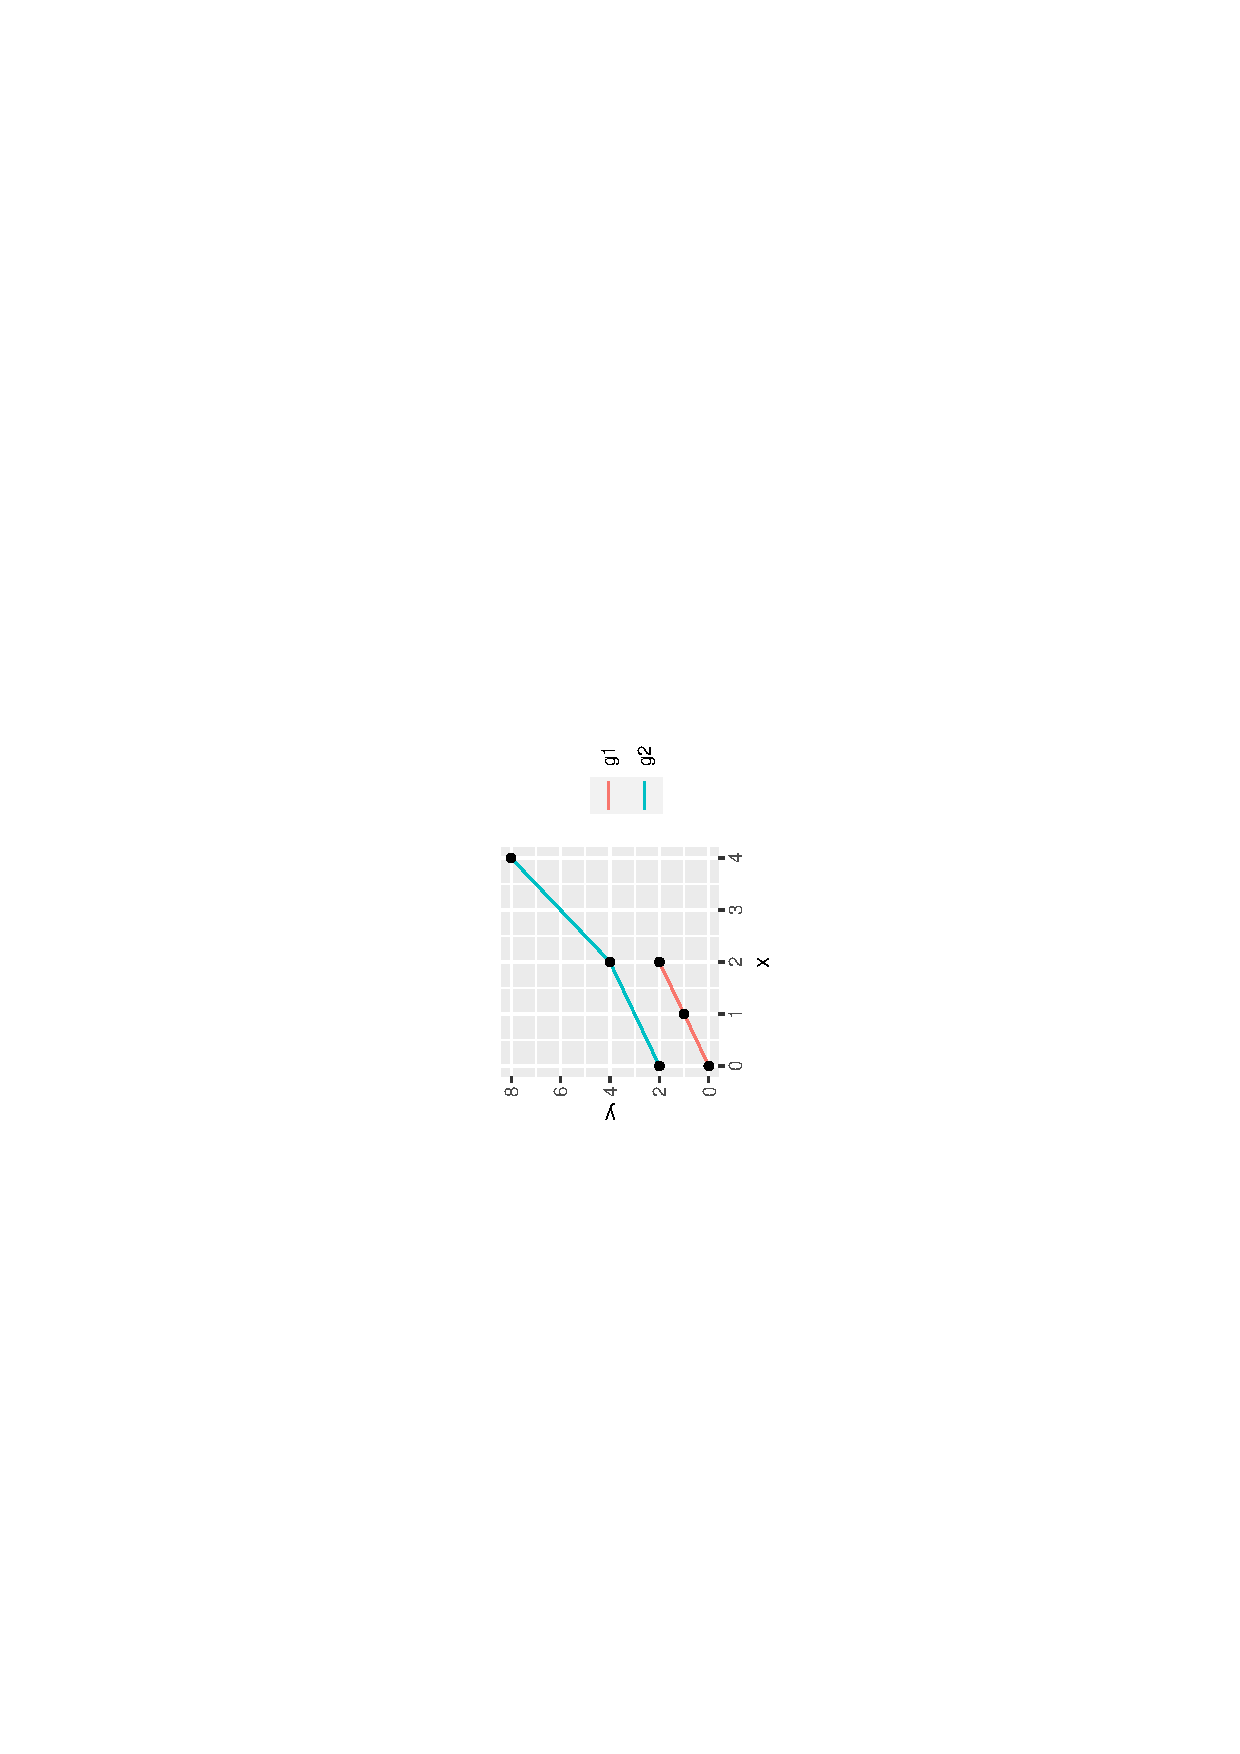
\includegraphics{plotLine}}}
    \end{tabular}
  \end{center}
  \caption{Example data (\textbf{A}) plotted with \ty{plotLine}
    (\textbf{B}).}\label{fig:plot}
\end{figure}

\section*{Implementation}
The outline of \ty{plotLine} has hooks for imports, types, functions,
and the logic of the main function.
\nwenddocs{}\nwbegincode{2}\sublabel{NW0-Xo4Ez-1}\nwmargintag{{\nwtagstyle{}\subpageref{NW0-Xo4Ez-1}}}\moddef{plotLine.go~{\nwtagstyle{}\subpageref{NW0-Xo4Ez-1}}}\endmoddef\nwstartdeflinemarkup\nwenddeflinemarkup
package main

import (
          \LA{}Imports, Ch.~\ref{ch:pl}~{\nwtagstyle{}\subpageref{NW0-2OMat3-1}}\RA{}
)
\LA{}Types, Ch.~\ref{ch:pl}~{\nwtagstyle{}\subpageref{NW0-HbCKE-1}}\RA{}
\LA{}Functions, Ch.~\ref{ch:pl}~{\nwtagstyle{}\subpageref{NW0-3njhFS-1}}\RA{}
func main() \{
          \LA{}Main function, Ch.~\ref{ch:pl}~{\nwtagstyle{}\subpageref{NW0-4WX4eM-1}}\RA{}
\}
\nwnotused{plotLine.go}\nwendcode{}\nwbegindocs{3}\nwdocspar
In the main function we set the usage, declare the options, parse the
options, and parse the input files.
\nwenddocs{}\nwbegincode{4}\sublabel{NW0-4WX4eM-1}\nwmargintag{{\nwtagstyle{}\subpageref{NW0-4WX4eM-1}}}\moddef{Main function, Ch.~\ref{ch:pl}~{\nwtagstyle{}\subpageref{NW0-4WX4eM-1}}}\endmoddef\nwstartdeflinemarkup\nwusesondefline{\\{NW0-Xo4Ez-1}}\nwenddeflinemarkup
\LA{}Set usage, Ch.~\ref{ch:pl}~{\nwtagstyle{}\subpageref{NW0-z3Bve-1}}\RA{}
\LA{}Declare options, Ch.~\ref{ch:pl}~{\nwtagstyle{}\subpageref{NW0-22PPLz-1}}\RA{}
\LA{}Parse options, Ch.~\ref{ch:pl}~{\nwtagstyle{}\subpageref{NW0-1mk760-1}}\RA{}
\LA{}Parse input files, Ch.~\ref{ch:pl}~{\nwtagstyle{}\subpageref{NW0-3D30ZY-1}}\RA{}
\nwused{\\{NW0-Xo4Ez-1}}\nwendcode{}\nwbegindocs{5}\nwdocspar
The usage consists of the actual usage message, an explanation of the
program's purpose, and an example command.
\nwenddocs{}\nwbegincode{6}\sublabel{NW0-z3Bve-1}\nwmargintag{{\nwtagstyle{}\subpageref{NW0-z3Bve-1}}}\moddef{Set usage, Ch.~\ref{ch:pl}~{\nwtagstyle{}\subpageref{NW0-z3Bve-1}}}\endmoddef\nwstartdeflinemarkup\nwusesondefline{\\{NW0-4WX4eM-1}}\nwenddeflinemarkup
u := "plotLine [-h] [option]... [file]..."
p := "Plot lines from columns of x/y data " +
          "and an optional group column."
e := "plotLine -x Time -y [RNA] foo.dat"
clio.Usage(u, p, e)
\nwused{\\{NW0-4WX4eM-1}}\nwendcode{}\nwbegindocs{7}\nwdocspar
We import \ty{clio}.
\nwenddocs{}\nwbegincode{8}\sublabel{NW0-2OMat3-1}\nwmargintag{{\nwtagstyle{}\subpageref{NW0-2OMat3-1}}}\moddef{Imports, Ch.~\ref{ch:pl}~{\nwtagstyle{}\subpageref{NW0-2OMat3-1}}}\endmoddef\nwstartdeflinemarkup\nwusesondefline{\\{NW0-Xo4Ez-1}}\nwprevnextdefs{\relax}{NW0-2OMat3-2}\nwenddeflinemarkup
"github.com/evolbioinf/clio"
\nwalsodefined{\\{NW0-2OMat3-2}\\{NW0-2OMat3-3}\\{NW0-2OMat3-4}\\{NW0-2OMat3-5}\\{NW0-2OMat3-6}\\{NW0-2OMat3-7}\\{NW0-2OMat3-8}\\{NW0-2OMat3-9}\\{NW0-2OMat3-A}\\{NW0-2OMat3-B}\\{NW0-2OMat3-C}}\nwused{\\{NW0-Xo4Ez-1}}\nwendcode{}\nwbegindocs{9}\nwdocspar
Apart from the version, we declare options concerning the axes, the
plot type, the graphics device, and the underlying R script.
\nwenddocs{}\nwbegincode{10}\sublabel{NW0-22PPLz-1}\nwmargintag{{\nwtagstyle{}\subpageref{NW0-22PPLz-1}}}\moddef{Declare options, Ch.~\ref{ch:pl}~{\nwtagstyle{}\subpageref{NW0-22PPLz-1}}}\endmoddef\nwstartdeflinemarkup\nwusesondefline{\\{NW0-4WX4eM-1}}\nwenddeflinemarkup
var optV = flag.Bool("v", false, "print program version " +
          "and other information")
\LA{}Declare axes options, Ch~\ref{ch:pl}~{\nwtagstyle{}\subpageref{NW0-3Gh3I0-1}}\RA{}
\LA{}Declare plot type options, Ch.~\ref{ch:pl}~{\nwtagstyle{}\subpageref{NW0-2Xy0v1-1}}\RA{}
\LA{}Declare device options, Ch.~\ref{ch:pl}~{\nwtagstyle{}\subpageref{NW0-26XxAt-1}}\RA{}
\LA{}Declare script options, Ch.~\ref{ch:pl}~{\nwtagstyle{}\subpageref{NW0-1Duv4j-1}}\RA{}
\nwused{\\{NW0-4WX4eM-1}}\nwendcode{}\nwbegindocs{11}\nwdocspar
We import \ty{flag}.
\nwenddocs{}\nwbegincode{12}\sublabel{NW0-2OMat3-2}\nwmargintag{{\nwtagstyle{}\subpageref{NW0-2OMat3-2}}}\moddef{Imports, Ch.~\ref{ch:pl}~{\nwtagstyle{}\subpageref{NW0-2OMat3-1}}}\plusendmoddef\nwstartdeflinemarkup\nwusesondefline{\\{NW0-Xo4Ez-1}}\nwprevnextdefs{NW0-2OMat3-1}{NW0-2OMat3-3}\nwenddeflinemarkup
"flag"
\nwused{\\{NW0-Xo4Ez-1}}\nwendcode{}\nwbegindocs{13}\nwdocspar
The options for axes define their labels, the range, and the scale.
\nwenddocs{}\nwbegincode{14}\sublabel{NW0-3Gh3I0-1}\nwmargintag{{\nwtagstyle{}\subpageref{NW0-3Gh3I0-1}}}\moddef{Declare axes options, Ch~\ref{ch:pl}~{\nwtagstyle{}\subpageref{NW0-3Gh3I0-1}}}\endmoddef\nwstartdeflinemarkup\nwusesondefline{\\{NW0-22PPLz-1}}\nwenddeflinemarkup
var optX = flag.String("x", "x", "x-label")
var optY = flag.String("y", "y", "y-label")
var optXX = flag.String("X", "s:e", "x-range")
var optYY = flag.String("Y", "s:e", "y-range")
var optL = flag.String("l", "", "log-scale (x|y|xy)")
\nwused{\\{NW0-22PPLz-1}}\nwendcode{}\nwbegindocs{15}\nwdocspar
The user can set the base size of the plot, and opt for dots only or
lines with dots.
\nwenddocs{}\nwbegincode{16}\sublabel{NW0-2Xy0v1-1}\nwmargintag{{\nwtagstyle{}\subpageref{NW0-2Xy0v1-1}}}\moddef{Declare plot type options, Ch.~\ref{ch:pl}~{\nwtagstyle{}\subpageref{NW0-2Xy0v1-1}}}\endmoddef\nwstartdeflinemarkup\nwusesondefline{\\{NW0-22PPLz-1}}\nwenddeflinemarkup
var optS = flag.Int("s", 0, "base size")
var optD = flag.Bool("d", false, "dots only")
var optDD = flag.Bool("D", false, "dots with lines")
\nwused{\\{NW0-22PPLz-1}}\nwendcode{}\nwbegindocs{17}\nwdocspar
The user can set the graphical device, and set the width and height of
the plot it produces. Among the graphical devices supported by R, we
recognize five:
\begin{itemize}
\item postscript (p)
\item PDF (P)
\item x11 (x)
\item quartz (q)
\item windows (w)
\end{itemize}
\nwenddocs{}\nwbegincode{18}\sublabel{NW0-26XxAt-1}\nwmargintag{{\nwtagstyle{}\subpageref{NW0-26XxAt-1}}}\moddef{Declare device options, Ch.~\ref{ch:pl}~{\nwtagstyle{}\subpageref{NW0-26XxAt-1}}}\endmoddef\nwstartdeflinemarkup\nwusesondefline{\\{NW0-22PPLz-1}}\nwenddeflinemarkup
var optG = flag.String("g", "x", "graphical device, " +
          "first character of x11, ps, PDF, quartz, windows")
var optW = flag.Float64("w", 0.0, "width in cm")
var optHH = flag.Float64("H", 0.0, "height in cm")
\nwused{\\{NW0-22PPLz-1}}\nwendcode{}\nwbegindocs{19}\nwdocspar
The R script used for plotting is not accessible to the user. However,
the user can opt to have it printed to a file.
\nwenddocs{}\nwbegincode{20}\sublabel{NW0-1Duv4j-1}\nwmargintag{{\nwtagstyle{}\subpageref{NW0-1Duv4j-1}}}\moddef{Declare script options, Ch.~\ref{ch:pl}~{\nwtagstyle{}\subpageref{NW0-1Duv4j-1}}}\endmoddef\nwstartdeflinemarkup\nwusesondefline{\\{NW0-22PPLz-1}}\nwenddeflinemarkup
var optR = flag.String("r", "", "file for R script")
\nwused{\\{NW0-22PPLz-1}}\nwendcode{}\nwbegindocs{21}\nwdocspar
We parse the options and respond to \ty{-v}, as this might terminate
the program. Then we collect the values of options that are straight
forward in the variable \ty{args}. What remains are the more complex
options \ty{-X}, \ty{-Y}, \ty{-g}, and \ty{-l}. We respond to each one
of these in turn.
\nwenddocs{}\nwbegincode{22}\sublabel{NW0-1mk760-1}\nwmargintag{{\nwtagstyle{}\subpageref{NW0-1mk760-1}}}\moddef{Parse options, Ch.~\ref{ch:pl}~{\nwtagstyle{}\subpageref{NW0-1mk760-1}}}\endmoddef\nwstartdeflinemarkup\nwusesondefline{\\{NW0-4WX4eM-1}}\nwenddeflinemarkup
flag.Parse()
\LA{}Respond to \ty{-v}, Ch.~\ref{ch:pl}~{\nwtagstyle{}\subpageref{NW0-1Ge4wP-1}}\RA{}
args := new(Args)
\LA{}Collect option values, Ch.~\ref{ch:pl}~{\nwtagstyle{}\subpageref{NW0-45cVO7-1}}\RA{}
\LA{}Respond to \ty{-X}, Ch.~\ref{ch:pl}~{\nwtagstyle{}\subpageref{NW0-49jiXL-1}}\RA{}
\LA{}Respond to \ty{-Y}, Ch.~\ref{ch:pl}~{\nwtagstyle{}\subpageref{NW0-2jxkg3-1}}\RA{}
\LA{}Respond to \ty{-g}, Ch.~\ref{ch:pl}~{\nwtagstyle{}\subpageref{NW0-325APy-1}}\RA{}
\LA{}Respond to \ty{-l}, Ch.~\ref{ch:pl}~{\nwtagstyle{}\subpageref{NW0-1lVsWW-1}}\RA{}
\nwused{\\{NW0-4WX4eM-1}}\nwendcode{}\nwbegindocs{23}\nwdocspar
We respond to \ty{-v} by printing a standardized message.
\nwenddocs{}\nwbegincode{24}\sublabel{NW0-1Ge4wP-1}\nwmargintag{{\nwtagstyle{}\subpageref{NW0-1Ge4wP-1}}}\moddef{Respond to \ty{-v}, Ch.~\ref{ch:pl}~{\nwtagstyle{}\subpageref{NW0-1Ge4wP-1}}}\endmoddef\nwstartdeflinemarkup\nwusesondefline{\\{NW0-1mk760-1}}\nwenddeflinemarkup
if *optV \{
          util.PrintInfo("plotLine")
\}
\nwused{\\{NW0-1mk760-1}}\nwendcode{}\nwbegindocs{25}\nwdocspar
We import \ty{util}.
\nwenddocs{}\nwbegincode{26}\sublabel{NW0-2OMat3-3}\nwmargintag{{\nwtagstyle{}\subpageref{NW0-2OMat3-3}}}\moddef{Imports, Ch.~\ref{ch:pl}~{\nwtagstyle{}\subpageref{NW0-2OMat3-1}}}\plusendmoddef\nwstartdeflinemarkup\nwusesondefline{\\{NW0-Xo4Ez-1}}\nwprevnextdefs{NW0-2OMat3-2}{NW0-2OMat3-4}\nwenddeflinemarkup
"github.com/evolbioinf/biobox/util"
\nwused{\\{NW0-Xo4Ez-1}}\nwendcode{}\nwbegindocs{27}\nwdocspar
We declare the type \ty{Args} and specify its fields as we go along.
\nwenddocs{}\nwbegincode{28}\sublabel{NW0-HbCKE-1}\nwmargintag{{\nwtagstyle{}\subpageref{NW0-HbCKE-1}}}\moddef{Types, Ch.~\ref{ch:pl}~{\nwtagstyle{}\subpageref{NW0-HbCKE-1}}}\endmoddef\nwstartdeflinemarkup\nwusesondefline{\\{NW0-Xo4Ez-1}}\nwenddeflinemarkup
type Args struct \{
          \LA{}\ty{Args} fields, Ch.~\ref{ch:pl}~{\nwtagstyle{}\subpageref{NW0-2Qrfrd-1}}\RA{}
\}
\nwused{\\{NW0-Xo4Ez-1}}\nwendcode{}\nwbegindocs{29}\nwdocspar
We collect the option values that require no further analysis,
\ty{-x}, \ty{-y}, \ty{-H}, \ty{-w}, \ty{-s}, \ty{-r}, \ty{-d}, and
\ty{-D}. Since R takes height and width in inches, we convert the cm
read.
\nwenddocs{}\nwbegincode{30}\sublabel{NW0-45cVO7-1}\nwmargintag{{\nwtagstyle{}\subpageref{NW0-45cVO7-1}}}\moddef{Collect option values, Ch.~\ref{ch:pl}~{\nwtagstyle{}\subpageref{NW0-45cVO7-1}}}\endmoddef\nwstartdeflinemarkup\nwusesondefline{\\{NW0-1mk760-1}}\nwenddeflinemarkup
args.Xlab = *optX
args.Ylab = *optY
args.Height = *optHH / 2.54
args.Width = *optW / 2.54
args.Size = *optS
args.Script = *optR
args.Dots = *optD
args.DotsLines = *optDD
\nwused{\\{NW0-1mk760-1}}\nwendcode{}\nwbegindocs{31}\nwdocspar
We add the corresponding fields to the structure \ty{Args}.
\nwenddocs{}\nwbegincode{32}\sublabel{NW0-2Qrfrd-1}\nwmargintag{{\nwtagstyle{}\subpageref{NW0-2Qrfrd-1}}}\moddef{\ty{Args} fields, Ch.~\ref{ch:pl}~{\nwtagstyle{}\subpageref{NW0-2Qrfrd-1}}}\endmoddef\nwstartdeflinemarkup\nwusesondefline{\\{NW0-HbCKE-1}}\nwprevnextdefs{\relax}{NW0-2Qrfrd-2}\nwenddeflinemarkup
Xlab, Ylab string
Height, Width float64
Size int
Script string
Dots, DotsLines bool
\nwalsodefined{\\{NW0-2Qrfrd-2}\\{NW0-2Qrfrd-3}\\{NW0-2Qrfrd-4}\\{NW0-2Qrfrd-5}\\{NW0-2Qrfrd-6}\\{NW0-2Qrfrd-7}}\nwused{\\{NW0-HbCKE-1}}\nwendcode{}\nwbegindocs{33}\nwdocspar
The \ty{-X} option contains the x-range as a string where start and
end are separated by a colon. If the user didn't set a range,
\ty{Xrange} keeps its default value, false.
\nwenddocs{}\nwbegincode{34}\sublabel{NW0-49jiXL-1}\nwmargintag{{\nwtagstyle{}\subpageref{NW0-49jiXL-1}}}\moddef{Respond to \ty{-X}, Ch.~\ref{ch:pl}~{\nwtagstyle{}\subpageref{NW0-49jiXL-1}}}\endmoddef\nwstartdeflinemarkup\nwusesondefline{\\{NW0-1mk760-1}}\nwenddeflinemarkup
sa := strings.Split(*optXX, ":")
var err error
if sa[0] != "s" && sa[1] != "e" \{
          args.Xmin, err = strconv.ParseFloat(sa[0], 64)
          if err != nil \{ log.Fatal(err.Error()) \}
          args.Xmax, err = strconv.ParseFloat(sa[1], 64)
          if err != nil \{ log.Fatal(err.Error()) \}
          args.Xrange = true
\}
\nwused{\\{NW0-1mk760-1}}\nwendcode{}\nwbegindocs{35}\nwdocspar
We import \ty{strings}, \ty{strconv}, and \ty{log}.
\nwenddocs{}\nwbegincode{36}\sublabel{NW0-2OMat3-4}\nwmargintag{{\nwtagstyle{}\subpageref{NW0-2OMat3-4}}}\moddef{Imports, Ch.~\ref{ch:pl}~{\nwtagstyle{}\subpageref{NW0-2OMat3-1}}}\plusendmoddef\nwstartdeflinemarkup\nwusesondefline{\\{NW0-Xo4Ez-1}}\nwprevnextdefs{NW0-2OMat3-3}{NW0-2OMat3-5}\nwenddeflinemarkup
"strings"
"strconv"
"log"
\nwused{\\{NW0-Xo4Ez-1}}\nwendcode{}\nwbegindocs{37}\nwdocspar
We add the new fields for the x-range to \ty{Args}.
\nwenddocs{}\nwbegincode{38}\sublabel{NW0-2Qrfrd-2}\nwmargintag{{\nwtagstyle{}\subpageref{NW0-2Qrfrd-2}}}\moddef{\ty{Args} fields, Ch.~\ref{ch:pl}~{\nwtagstyle{}\subpageref{NW0-2Qrfrd-1}}}\plusendmoddef\nwstartdeflinemarkup\nwusesondefline{\\{NW0-HbCKE-1}}\nwprevnextdefs{NW0-2Qrfrd-1}{NW0-2Qrfrd-3}\nwenddeflinemarkup
Xmin, Xmax float64
Xrange bool
\nwused{\\{NW0-HbCKE-1}}\nwendcode{}\nwbegindocs{39}\nwdocspar
We also convert the y-range to numbers.
\nwenddocs{}\nwbegincode{40}\sublabel{NW0-2jxkg3-1}\nwmargintag{{\nwtagstyle{}\subpageref{NW0-2jxkg3-1}}}\moddef{Respond to \ty{-Y}, Ch.~\ref{ch:pl}~{\nwtagstyle{}\subpageref{NW0-2jxkg3-1}}}\endmoddef\nwstartdeflinemarkup\nwusesondefline{\\{NW0-1mk760-1}}\nwenddeflinemarkup
sa = strings.Split(*optYY, ":")
if sa[0] != "s" && sa[1] != "e" \{
          args.Ymin, err = strconv.ParseFloat(sa[0], 64)
          if err != nil \{ log.Fatal(err.Error()) \}
          args.Ymax, err = strconv.ParseFloat(sa[1], 64)
          if err != nil \{ log.Fatal(err.Error()) \}
          args.Yrange = true
\}
\nwused{\\{NW0-1mk760-1}}\nwendcode{}\nwbegindocs{41}\nwdocspar
We add the new fields for the y-range to \ty{Args}.
\nwenddocs{}\nwbegincode{42}\sublabel{NW0-2Qrfrd-3}\nwmargintag{{\nwtagstyle{}\subpageref{NW0-2Qrfrd-3}}}\moddef{\ty{Args} fields, Ch.~\ref{ch:pl}~{\nwtagstyle{}\subpageref{NW0-2Qrfrd-1}}}\plusendmoddef\nwstartdeflinemarkup\nwusesondefline{\\{NW0-HbCKE-1}}\nwprevnextdefs{NW0-2Qrfrd-2}{NW0-2Qrfrd-4}\nwenddeflinemarkup
Ymin, Ymax float64
Yrange bool
\nwused{\\{NW0-HbCKE-1}}\nwendcode{}\nwbegindocs{43}\nwdocspar
Among the graphical devices, we first deal with the screen devices,
then with the file devices.
\nwenddocs{}\nwbegincode{44}\sublabel{NW0-325APy-1}\nwmargintag{{\nwtagstyle{}\subpageref{NW0-325APy-1}}}\moddef{Respond to \ty{-g}, Ch.~\ref{ch:pl}~{\nwtagstyle{}\subpageref{NW0-325APy-1}}}\endmoddef\nwstartdeflinemarkup\nwusesondefline{\\{NW0-1mk760-1}}\nwenddeflinemarkup
switch *optG \{
          \LA{}Deal with screen devices, Ch.~\ref{ch:pl}~{\nwtagstyle{}\subpageref{NW0-net1l-1}}\RA{}
          \LA{}Deal with file devices, Ch.~\ref{ch:pl}~{\nwtagstyle{}\subpageref{NW0-oxRsG-1}}\RA{}
\}
\nwused{\\{NW0-1mk760-1}}\nwendcode{}\nwbegindocs{45}\nwdocspar
We go through the two file devices.
\nwenddocs{}\nwbegincode{46}\sublabel{NW0-oxRsG-1}\nwmargintag{{\nwtagstyle{}\subpageref{NW0-oxRsG-1}}}\moddef{Deal with file devices, Ch.~\ref{ch:pl}~{\nwtagstyle{}\subpageref{NW0-oxRsG-1}}}\endmoddef\nwstartdeflinemarkup\nwusesondefline{\\{NW0-325APy-1}}\nwenddeflinemarkup
case "p":
args.Graph = "postscript"
case "P":
args.Graph = "pdf"
\nwused{\\{NW0-325APy-1}}\nwendcode{}\nwbegindocs{47}\nwdocspar
We add the field \ty{Graph} to \ty{Args}.
\nwenddocs{}\nwbegincode{48}\sublabel{NW0-2Qrfrd-4}\nwmargintag{{\nwtagstyle{}\subpageref{NW0-2Qrfrd-4}}}\moddef{\ty{Args} fields, Ch.~\ref{ch:pl}~{\nwtagstyle{}\subpageref{NW0-2Qrfrd-1}}}\plusendmoddef\nwstartdeflinemarkup\nwusesondefline{\\{NW0-HbCKE-1}}\nwprevnextdefs{NW0-2Qrfrd-3}{NW0-2Qrfrd-5}\nwenddeflinemarkup
Graph string
\nwused{\\{NW0-HbCKE-1}}\nwendcode{}\nwbegindocs{49}\nwdocspar
The screen devices also contain the default, X11. And given that file
and screen devices are treated differently in R, we also not whether
or not they are screen devices.
\nwenddocs{}\nwbegincode{50}\sublabel{NW0-net1l-1}\nwmargintag{{\nwtagstyle{}\subpageref{NW0-net1l-1}}}\moddef{Deal with screen devices, Ch.~\ref{ch:pl}~{\nwtagstyle{}\subpageref{NW0-net1l-1}}}\endmoddef\nwstartdeflinemarkup\nwusesondefline{\\{NW0-325APy-1}}\nwenddeflinemarkup
case "q":
args.Graph = "quartz"
args.Screen = true
case "w":
args.Graph = "windows"
args.Screen = true
default:
args.Graph = "X11"
args.Screen = true
\nwused{\\{NW0-325APy-1}}\nwendcode{}\nwbegindocs{51}\nwdocspar
We add the field \ty{Screen} to \ty{Args}.
\nwenddocs{}\nwbegincode{52}\sublabel{NW0-2Qrfrd-5}\nwmargintag{{\nwtagstyle{}\subpageref{NW0-2Qrfrd-5}}}\moddef{\ty{Args} fields, Ch.~\ref{ch:pl}~{\nwtagstyle{}\subpageref{NW0-2Qrfrd-1}}}\plusendmoddef\nwstartdeflinemarkup\nwusesondefline{\\{NW0-HbCKE-1}}\nwprevnextdefs{NW0-2Qrfrd-4}{NW0-2Qrfrd-6}\nwenddeflinemarkup
Screen bool
\nwused{\\{NW0-HbCKE-1}}\nwendcode{}\nwbegindocs{53}\nwdocspar
If the user submitted an unknown graphical device, there is probably
something wrong and we bail with a friendly message.
\nwenddocs{}\nwbegincode{54}\sublabel{NW0-3vOttg-1}\nwmargintag{{\nwtagstyle{}\subpageref{NW0-3vOttg-1}}}\moddef{Respond to unknown graphical device, Ch.~\ref{ch:pl}~{\nwtagstyle{}\subpageref{NW0-3vOttg-1}}}\endmoddef\nwstartdeflinemarkup\nwenddeflinemarkup
log.Fatalf("%s refers to an unknown " +
          "graphical device\\n", *optG)
\nwnotused{Respond to unknown graphical device, Ch.~\ref{ch:pl}}\nwendcode{}\nwbegindocs{55}\nwdocspar
The log-option is a small integer, where 0 denotes linear, 1
x-log, 2 y-log, and 3 xy-log.
\nwenddocs{}\nwbegincode{56}\sublabel{NW0-1lVsWW-1}\nwmargintag{{\nwtagstyle{}\subpageref{NW0-1lVsWW-1}}}\moddef{Respond to \ty{-l}, Ch.~\ref{ch:pl}~{\nwtagstyle{}\subpageref{NW0-1lVsWW-1}}}\endmoddef\nwstartdeflinemarkup\nwusesondefline{\\{NW0-1mk760-1}}\nwenddeflinemarkup
if *optL == "x" || *optL == "X" \{
          args.Log = 1
\} else if *optL == "y" || *optL == "Y" \{
          args.Log = 2
\} else if ok, err := regexp.MatchString(`^[xX][yY]$`, *optL);
err == nil && ok \{
          args.Log = 3
\}
\nwused{\\{NW0-1mk760-1}}\nwendcode{}\nwbegindocs{57}\nwdocspar
We import \ty{regexp}.
\nwenddocs{}\nwbegincode{58}\sublabel{NW0-2OMat3-5}\nwmargintag{{\nwtagstyle{}\subpageref{NW0-2OMat3-5}}}\moddef{Imports, Ch.~\ref{ch:pl}~{\nwtagstyle{}\subpageref{NW0-2OMat3-1}}}\plusendmoddef\nwstartdeflinemarkup\nwusesondefline{\\{NW0-Xo4Ez-1}}\nwprevnextdefs{NW0-2OMat3-4}{NW0-2OMat3-6}\nwenddeflinemarkup
"regexp"
\nwused{\\{NW0-Xo4Ez-1}}\nwendcode{}\nwbegindocs{59}\nwdocspar
\ty{Args} gets the log field.
\nwenddocs{}\nwbegincode{60}\sublabel{NW0-2Qrfrd-6}\nwmargintag{{\nwtagstyle{}\subpageref{NW0-2Qrfrd-6}}}\moddef{\ty{Args} fields, Ch.~\ref{ch:pl}~{\nwtagstyle{}\subpageref{NW0-2Qrfrd-1}}}\plusendmoddef\nwstartdeflinemarkup\nwusesondefline{\\{NW0-HbCKE-1}}\nwprevnextdefs{NW0-2Qrfrd-5}{NW0-2Qrfrd-7}\nwenddeflinemarkup
Log byte
\nwused{\\{NW0-HbCKE-1}}\nwendcode{}\nwbegindocs{61}\nwdocspar
We import \ty{regexp}.
\nwenddocs{}\nwbegincode{62}\sublabel{NW0-2OMat3-6}\nwmargintag{{\nwtagstyle{}\subpageref{NW0-2OMat3-6}}}\moddef{Imports, Ch.~\ref{ch:pl}~{\nwtagstyle{}\subpageref{NW0-2OMat3-1}}}\plusendmoddef\nwstartdeflinemarkup\nwusesondefline{\\{NW0-Xo4Ez-1}}\nwprevnextdefs{NW0-2OMat3-5}{NW0-2OMat3-7}\nwenddeflinemarkup
"regexp"
\nwused{\\{NW0-Xo4Ez-1}}\nwendcode{}\nwbegindocs{63}\nwdocspar
The remaining tokens on the command line are taken as input
files. These are parsed with the function \ty{ParseFiles}, which
subjects each file to the function \ty{scan}. \ty{scan}, in turn,
takes as argument the arguments we just collected.
\nwenddocs{}\nwbegincode{64}\sublabel{NW0-3D30ZY-1}\nwmargintag{{\nwtagstyle{}\subpageref{NW0-3D30ZY-1}}}\moddef{Parse input files, Ch.~\ref{ch:pl}~{\nwtagstyle{}\subpageref{NW0-3D30ZY-1}}}\endmoddef\nwstartdeflinemarkup\nwusesondefline{\\{NW0-4WX4eM-1}}\nwenddeflinemarkup
files := flag.Args()
clio.ParseFiles(files, scan, args)
\nwused{\\{NW0-4WX4eM-1}}\nwendcode{}\nwbegindocs{65}\nwdocspar
Inside \ty{scan}, we retrieve the options, read the data, construct
the R script, construct the R command that runs the script, pipe the
data into it, and run it. Then we delete the R script again, unless
the user wrote it to a specific file.
\nwenddocs{}\nwbegincode{66}\sublabel{NW0-3njhFS-1}\nwmargintag{{\nwtagstyle{}\subpageref{NW0-3njhFS-1}}}\moddef{Functions, Ch.~\ref{ch:pl}~{\nwtagstyle{}\subpageref{NW0-3njhFS-1}}}\endmoddef\nwstartdeflinemarkup\nwusesondefline{\\{NW0-Xo4Ez-1}}\nwenddeflinemarkup
func scan(r io.Reader, a ...interface\{\}) \{
          args := a[0].(*Args)
          \LA{}Read data, Ch.~\ref{ch:pl}~{\nwtagstyle{}\subpageref{NW0-vBH4f-1}}\RA{}
          \LA{}Construct R script, Ch.~\ref{ch:pl}~{\nwtagstyle{}\subpageref{NW0-21c6x4-1}}\RA{}
          \LA{}Construct R command, Ch.~\ref{ch:pl}~{\nwtagstyle{}\subpageref{NW0-3yi03G-1}}\RA{}
          \LA{}Pipe data into R command, Ch.~\ref{ch:pl}~{\nwtagstyle{}\subpageref{NW0-4LFgkU-1}}\RA{}
          \LA{}Run R command, Ch.~\ref{ch:pl}~{\nwtagstyle{}\subpageref{NW0-3i8K6I-1}}\RA{}
          if args.Script == "" \{
                  \LA{}Delete R script, Ch.~\ref{ch:pl}~{\nwtagstyle{}\subpageref{NW0-35YheO-1}}\RA{}
          \}
\}
\nwused{\\{NW0-Xo4Ez-1}}\nwendcode{}\nwbegindocs{67}\nwdocspar
We import \ty{io}.
\nwenddocs{}\nwbegincode{68}\sublabel{NW0-2OMat3-7}\nwmargintag{{\nwtagstyle{}\subpageref{NW0-2OMat3-7}}}\moddef{Imports, Ch.~\ref{ch:pl}~{\nwtagstyle{}\subpageref{NW0-2OMat3-1}}}\plusendmoddef\nwstartdeflinemarkup\nwusesondefline{\\{NW0-Xo4Ez-1}}\nwprevnextdefs{NW0-2OMat3-6}{NW0-2OMat3-8}\nwenddeflinemarkup
"io"
\nwused{\\{NW0-Xo4Ez-1}}\nwendcode{}\nwbegindocs{69}\nwdocspar
While reading the data, we determine the number of columns from the
first row. The number of columns influences the plotting later, so we
save it with the other arguments. If the number of columns isn't 2 or
3, something has gone wrong and we stop reading. We'll respond more
fully to this case in a moment, when we construct the R script.
\nwenddocs{}\nwbegincode{70}\sublabel{NW0-vBH4f-1}\nwmargintag{{\nwtagstyle{}\subpageref{NW0-vBH4f-1}}}\moddef{Read data, Ch.~\ref{ch:pl}~{\nwtagstyle{}\subpageref{NW0-vBH4f-1}}}\endmoddef\nwstartdeflinemarkup\nwusesondefline{\\{NW0-3njhFS-1}}\nwenddeflinemarkup
var data []string
sc := bufio.NewScanner(r)
first := true
for sc.Scan() \{
          if first \{
                  first = false
                  args.Ncol = len(strings.Fields(sc.Text()))
          \}
          if args.Ncol < 2 || args.Ncol > 3 \{ break \}
          data = append(data, sc.Text())
\}
\nwused{\\{NW0-3njhFS-1}}\nwendcode{}\nwbegindocs{71}\nwdocspar
We import \ty{bufio}.
\nwenddocs{}\nwbegincode{72}\sublabel{NW0-2OMat3-8}\nwmargintag{{\nwtagstyle{}\subpageref{NW0-2OMat3-8}}}\moddef{Imports, Ch.~\ref{ch:pl}~{\nwtagstyle{}\subpageref{NW0-2OMat3-1}}}\plusendmoddef\nwstartdeflinemarkup\nwusesondefline{\\{NW0-Xo4Ez-1}}\nwprevnextdefs{NW0-2OMat3-7}{NW0-2OMat3-9}\nwenddeflinemarkup
"bufio"
\nwused{\\{NW0-Xo4Ez-1}}\nwendcode{}\nwbegindocs{73}\nwdocspar
We add \ty{Ncol} to \ty{Args}.
\nwenddocs{}\nwbegincode{74}\sublabel{NW0-2Qrfrd-7}\nwmargintag{{\nwtagstyle{}\subpageref{NW0-2Qrfrd-7}}}\moddef{\ty{Args} fields, Ch.~\ref{ch:pl}~{\nwtagstyle{}\subpageref{NW0-2Qrfrd-1}}}\plusendmoddef\nwstartdeflinemarkup\nwusesondefline{\\{NW0-HbCKE-1}}\nwprevnextdefs{NW0-2Qrfrd-6}{\relax}\nwenddeflinemarkup
Ncol int
\nwused{\\{NW0-HbCKE-1}}\nwendcode{}\nwbegindocs{75}\nwdocspar
We open a file to write the script to. But before actually doing that,
we make sure the input data has either two or three columns.
\nwenddocs{}\nwbegincode{76}\sublabel{NW0-21c6x4-1}\nwmargintag{{\nwtagstyle{}\subpageref{NW0-21c6x4-1}}}\moddef{Construct R script, Ch.~\ref{ch:pl}~{\nwtagstyle{}\subpageref{NW0-21c6x4-1}}}\endmoddef\nwstartdeflinemarkup\nwusesondefline{\\{NW0-3njhFS-1}}\nwenddeflinemarkup
\LA{}Open script file, Ch.~\ref{ch:pl}~{\nwtagstyle{}\subpageref{NW0-25TzRq-1}}\RA{}
if args.Ncol == 2 || args.Ncol == 3 \{
          \LA{}Deal with two or three columns, Ch.~\ref{ch:pl}~{\nwtagstyle{}\subpageref{NW0-10j8et-1}}\RA{}
\} else \{
          \LA{}Deal with wrong number of columns, Ch.~\ref{ch:pl}~{\nwtagstyle{}\subpageref{NW0-1s3swh-1}}\RA{}
\}
\nwused{\\{NW0-3njhFS-1}}\nwendcode{}\nwbegindocs{77}\nwdocspar
The script is written either to a unique file or to the file supplied
by the user. 
\nwenddocs{}\nwbegincode{78}\sublabel{NW0-25TzRq-1}\nwmargintag{{\nwtagstyle{}\subpageref{NW0-25TzRq-1}}}\moddef{Open script file, Ch.~\ref{ch:pl}~{\nwtagstyle{}\subpageref{NW0-25TzRq-1}}}\endmoddef\nwstartdeflinemarkup\nwusesondefline{\\{NW0-21c6x4-1}}\nwenddeflinemarkup
var script *os.File
var err error
if args.Script == "" \{
          script, err = ioutil.TempFile(".", "tmp_*.r")
\} else \{
          script, err = os.Create(args.Script)
\}
if err != nil \{
          log.Fatal(err.Error())
\}
\nwused{\\{NW0-21c6x4-1}}\nwendcode{}\nwbegindocs{79}\nwdocspar
We import \ty{ioutil}.
\nwenddocs{}\nwbegincode{80}\sublabel{NW0-2OMat3-9}\nwmargintag{{\nwtagstyle{}\subpageref{NW0-2OMat3-9}}}\moddef{Imports, Ch.~\ref{ch:pl}~{\nwtagstyle{}\subpageref{NW0-2OMat3-1}}}\plusendmoddef\nwstartdeflinemarkup\nwusesondefline{\\{NW0-Xo4Ez-1}}\nwprevnextdefs{NW0-2OMat3-8}{NW0-2OMat3-A}\nwenddeflinemarkup
"io/ioutil"
\nwused{\\{NW0-Xo4Ez-1}}\nwendcode{}\nwbegindocs{81}\nwdocspar
If the data has the wrong number of columns, there's bound to be
something wrong, so we bail with a friendly message.
\nwenddocs{}\nwbegincode{82}\sublabel{NW0-1s3swh-1}\nwmargintag{{\nwtagstyle{}\subpageref{NW0-1s3swh-1}}}\moddef{Deal with wrong number of columns, Ch.~\ref{ch:pl}~{\nwtagstyle{}\subpageref{NW0-1s3swh-1}}}\endmoddef\nwstartdeflinemarkup\nwusesondefline{\\{NW0-21c6x4-1}}\nwenddeflinemarkup
m := "there should be 2 or 3 columns " +
          "in the input, but you have %d\\n"
log.Fatalf(m, args.Ncol)
\nwused{\\{NW0-21c6x4-1}}\nwendcode{}\nwbegindocs{83}\nwdocspar
If there are two or three columns, we write the script using a
template, which we still have to create. Then we close the script
again.
\nwenddocs{}\nwbegincode{84}\sublabel{NW0-10j8et-1}\nwmargintag{{\nwtagstyle{}\subpageref{NW0-10j8et-1}}}\moddef{Deal with two or three columns, Ch.~\ref{ch:pl}~{\nwtagstyle{}\subpageref{NW0-10j8et-1}}}\endmoddef\nwstartdeflinemarkup\nwusesondefline{\\{NW0-21c6x4-1}}\nwenddeflinemarkup
tmpl := template.New("tmpl")
\LA{}Create template, Ch.~\ref{ch:pl}~{\nwtagstyle{}\subpageref{NW0-1Gsqae-1}}\RA{}
if err != nil \{
          log.Fatal(err.Error())
\}
err = tmpl.Execute(script, args)
if err != nil \{
          log.Fatal(err.Error())
\}
script.Close()
\nwused{\\{NW0-21c6x4-1}}\nwendcode{}\nwbegindocs{85}\nwdocspar
We import \ty{template}.
\nwenddocs{}\nwbegincode{86}\sublabel{NW0-2OMat3-A}\nwmargintag{{\nwtagstyle{}\subpageref{NW0-2OMat3-A}}}\moddef{Imports, Ch.~\ref{ch:pl}~{\nwtagstyle{}\subpageref{NW0-2OMat3-1}}}\plusendmoddef\nwstartdeflinemarkup\nwusesondefline{\\{NW0-Xo4Ez-1}}\nwprevnextdefs{NW0-2OMat3-9}{NW0-2OMat3-B}\nwenddeflinemarkup
"text/template"
\nwused{\\{NW0-Xo4Ez-1}}\nwendcode{}\nwbegindocs{87}\nwdocspar
The template is a string that then gets parsed.
\nwenddocs{}\nwbegincode{88}\sublabel{NW0-1Gsqae-1}\nwmargintag{{\nwtagstyle{}\subpageref{NW0-1Gsqae-1}}}\moddef{Create template, Ch.~\ref{ch:pl}~{\nwtagstyle{}\subpageref{NW0-1Gsqae-1}}}\endmoddef\nwstartdeflinemarkup\nwusesondefline{\\{NW0-10j8et-1}}\nwenddeflinemarkup
ts := ""
\LA{}Construct template string, Ch.~\ref{ch:pl}~{\nwtagstyle{}\subpageref{NW0-4HXEse-1}}\RA{}
tmpl = template.Must(tmpl.Parse(ts))
\nwused{\\{NW0-10j8et-1}}\nwendcode{}\nwbegindocs{89}\nwdocspar
We construct the template string in five steps. Construct the header,
construct the plot, and deal with the three plocks of options
affecting the axes, the plot type, and the plot device.
\nwenddocs{}\nwbegincode{90}\sublabel{NW0-4HXEse-1}\nwmargintag{{\nwtagstyle{}\subpageref{NW0-4HXEse-1}}}\moddef{Construct template string, Ch.~\ref{ch:pl}~{\nwtagstyle{}\subpageref{NW0-4HXEse-1}}}\endmoddef\nwstartdeflinemarkup\nwusesondefline{\\{NW0-1Gsqae-1}}\nwenddeflinemarkup
\LA{}Construct header, Ch.~\ref{ch:pl}~{\nwtagstyle{}\subpageref{NW0-4cDDUz-1}}\RA{}
\LA{}Construct plot, Ch.~\ref{ch:pl}~{\nwtagstyle{}\subpageref{NW0-3hHBeT-1}}\RA{}
\LA{}Deal with axes options, Ch.~\ref{ch:pl}~{\nwtagstyle{}\subpageref{NW0-305bxD-1}}\RA{}
\LA{}Deal with plot type options, Ch.~\ref{ch:pl}~{\nwtagstyle{}\subpageref{NW0-5YxPI-1}}\RA{}
\LA{}Deal with device options, Ch.~\ref{ch:pl}~{\nwtagstyle{}\subpageref{NW0-1CuRHs-1}}\RA{}
\nwused{\\{NW0-1Gsqae-1}}\nwendcode{}\nwbegindocs{91}\nwdocspar
In the header of the script, we load the ggplot2 library and read the
data from the standard input stream.
\nwenddocs{}\nwbegincode{92}\sublabel{NW0-4cDDUz-1}\nwmargintag{{\nwtagstyle{}\subpageref{NW0-4cDDUz-1}}}\moddef{Construct header, Ch.~\ref{ch:pl}~{\nwtagstyle{}\subpageref{NW0-4cDDUz-1}}}\endmoddef\nwstartdeflinemarkup\nwusesondefline{\\{NW0-4HXEse-1}}\nwenddeflinemarkup
ts = "library(\\"ggplot2\\")\\n"
ts += "data <- read.table(file=\\"stdin\\")\\n"
\nwused{\\{NW0-4HXEse-1}}\nwendcode{}\nwbegindocs{93}\nwdocspar
We construct the plot and group the data if there are three columns.
\nwenddocs{}\nwbegincode{94}\sublabel{NW0-3hHBeT-1}\nwmargintag{{\nwtagstyle{}\subpageref{NW0-3hHBeT-1}}}\moddef{Construct plot, Ch.~\ref{ch:pl}~{\nwtagstyle{}\subpageref{NW0-3hHBeT-1}}}\endmoddef\nwstartdeflinemarkup\nwusesondefline{\\{NW0-4HXEse-1}}\nwenddeflinemarkup
ts += "plot <- ggplot(data, aes(V1, V2\\n"
ts += "\{\{- if eq .Ncol 3\}\}, group=V3\{\{end\}\}))\\n"
\nwused{\\{NW0-4HXEse-1}}\nwendcode{}\nwbegindocs{95}\nwdocspar
We set the axis labels. If we have groups, we mark them with colors,
for which we shall use the variable \ty{color}. However, the
categories indicated by the colors are just the factors extracted from
V3. We don't want something like ``factor(V3)''as the label of the
groups table, so we set it to the empty string.
\nwenddocs{}\nwbegincode{96}\sublabel{NW0-305bxD-1}\nwmargintag{{\nwtagstyle{}\subpageref{NW0-305bxD-1}}}\moddef{Deal with axes options, Ch.~\ref{ch:pl}~{\nwtagstyle{}\subpageref{NW0-305bxD-1}}}\endmoddef\nwstartdeflinemarkup\nwusesondefline{\\{NW0-4HXEse-1}}\nwprevnextdefs{\relax}{NW0-305bxD-2}\nwenddeflinemarkup
ts += "plot <- plot + labs(x=\\"\{\{.Xlab\}\}\\", y=\\"\{\{.Ylab\}\}\\"\\n"
ts += "\{\{- if eq .Ncol 3 -\}\}\\n"
ts += ", color=\\"\\"\\n"
ts += "\{\{- end\}\})\\n"
\nwalsodefined{\\{NW0-305bxD-2}\\{NW0-305bxD-3}}\nwused{\\{NW0-4HXEse-1}}\nwendcode{}\nwbegindocs{97}\nwdocspar
We set the ranges, if available.
\nwenddocs{}\nwbegincode{98}\sublabel{NW0-305bxD-2}\nwmargintag{{\nwtagstyle{}\subpageref{NW0-305bxD-2}}}\moddef{Deal with axes options, Ch.~\ref{ch:pl}~{\nwtagstyle{}\subpageref{NW0-305bxD-1}}}\plusendmoddef\nwstartdeflinemarkup\nwusesondefline{\\{NW0-4HXEse-1}}\nwprevnextdefs{NW0-305bxD-1}{NW0-305bxD-3}\nwenddeflinemarkup
ts += "\{\{if .Xrange -\}\}\\n"
ts += "plot <- plot + xlim(\{\{.Xmin\}\}, \{\{.Xmax\}\})\\n"
ts += "\{\{end -\}\}\\n"
ts += "\{\{if .Yrange\}\}\\n"
ts += "plot <- plot + ylim(\{\{.Ymin\}\}, \{\{.Ymax\}\})\\n"
ts += "\{\{end -\}\}\\n"
\nwused{\\{NW0-4HXEse-1}}\nwendcode{}\nwbegindocs{99}\nwdocspar
We set the requested axes to log scale.
\nwenddocs{}\nwbegincode{100}\sublabel{NW0-305bxD-3}\nwmargintag{{\nwtagstyle{}\subpageref{NW0-305bxD-3}}}\moddef{Deal with axes options, Ch.~\ref{ch:pl}~{\nwtagstyle{}\subpageref{NW0-305bxD-1}}}\plusendmoddef\nwstartdeflinemarkup\nwusesondefline{\\{NW0-4HXEse-1}}\nwprevnextdefs{NW0-305bxD-2}{\relax}\nwenddeflinemarkup
ts += "\{\{if or (eq 1 .Log) (eq 3 .Log) -\}\}\\n"
ts += "plot <- plot + scale_x_log10()\\n"
ts += "\{\{end -\}\}\\n"
ts += "\{\{if or (eq 2 .Log) (eq 3 .Log) -\}\}\\n"
ts += "plot <- plot + scale_y_log10()\\n"
ts += "\{\{end -\}\}\\n"
\nwused{\\{NW0-4HXEse-1}}\nwendcode{}\nwbegindocs{101}\nwdocspar
The first of the plot type options we transcribe to R is the base
size of the plot.
\nwenddocs{}\nwbegincode{102}\sublabel{NW0-5YxPI-1}\nwmargintag{{\nwtagstyle{}\subpageref{NW0-5YxPI-1}}}\moddef{Deal with plot type options, Ch.~\ref{ch:pl}~{\nwtagstyle{}\subpageref{NW0-5YxPI-1}}}\endmoddef\nwstartdeflinemarkup\nwusesondefline{\\{NW0-4HXEse-1}}\nwprevnextdefs{\relax}{NW0-5YxPI-2}\nwenddeflinemarkup
ts += "\{\{if .Size -\}\}\\n"
ts += "plot <- plot + theme_grey(base_size=\{\{.Size\}\})\\n"
ts += "\{\{end -\}\}\\n"
\nwalsodefined{\\{NW0-5YxPI-2}\\{NW0-5YxPI-3}}\nwused{\\{NW0-4HXEse-1}}\nwendcode{}\nwbegindocs{103}\nwdocspar
The user might have requested that only dots be plotted. If not, we
plot lines. In either case we check whether there are three columns of
input data, in which case we extract the groups from the third column.
\nwenddocs{}\nwbegincode{104}\sublabel{NW0-5YxPI-2}\nwmargintag{{\nwtagstyle{}\subpageref{NW0-5YxPI-2}}}\moddef{Deal with plot type options, Ch.~\ref{ch:pl}~{\nwtagstyle{}\subpageref{NW0-5YxPI-1}}}\plusendmoddef\nwstartdeflinemarkup\nwusesondefline{\\{NW0-4HXEse-1}}\nwprevnextdefs{NW0-5YxPI-1}{NW0-5YxPI-3}\nwenddeflinemarkup
ts += "\{\{if .Dots -\}\}\\n"
ts += "plot <- plot + geom_point(\\n"
ts += "\{\{- if eq .Ncol 3 -\}\}\\n"
ts += "aes(color=factor(V3))\\n"
ts += "\{\{end -\}\})\\n"
ts += "\{\{else -\}\}\\n"
ts += "plot <- plot + geom_line(\\n"
ts += "\{\{- if eq .Ncol 3 -\}\}\\n"
ts += "aes(color=factor(V3))\\n"
ts += "\{\{- end\}\})\\n"
ts += "\{\{end -\}\}\\n"
\nwused{\\{NW0-4HXEse-1}}\nwendcode{}\nwbegindocs{105}\nwdocspar
The user might have requested points with the lines.
\nwenddocs{}\nwbegincode{106}\sublabel{NW0-5YxPI-3}\nwmargintag{{\nwtagstyle{}\subpageref{NW0-5YxPI-3}}}\moddef{Deal with plot type options, Ch.~\ref{ch:pl}~{\nwtagstyle{}\subpageref{NW0-5YxPI-1}}}\plusendmoddef\nwstartdeflinemarkup\nwusesondefline{\\{NW0-4HXEse-1}}\nwprevnextdefs{NW0-5YxPI-2}{\relax}\nwenddeflinemarkup
ts += "\{\{if .DotsLines -\}\}\\n"
ts += "plot <- plot + geom_point()\\n"
ts += "\{\{end -\}\}\\n"
\nwused{\\{NW0-4HXEse-1}}\nwendcode{}\nwbegindocs{107}\nwdocspar
We set up the graphical device, set its width and height, plot, and
close the device again.
\nwenddocs{}\nwbegincode{108}\sublabel{NW0-1CuRHs-1}\nwmargintag{{\nwtagstyle{}\subpageref{NW0-1CuRHs-1}}}\moddef{Deal with device options, Ch.~\ref{ch:pl}~{\nwtagstyle{}\subpageref{NW0-1CuRHs-1}}}\endmoddef\nwstartdeflinemarkup\nwusesondefline{\\{NW0-4HXEse-1}}\nwenddeflinemarkup
ts += "\{\{.Graph\}\}(\\n"
\LA{}Set width and height, Ch.~\ref{ch:pl}~{\nwtagstyle{}\subpageref{NW0-4VhtF6-1}}\RA{}
ts += "plot(plot)\\n"
\LA{}Close device, Ch.~\ref{ch:pl}~{\nwtagstyle{}\subpageref{NW0-3lzJL1-1}}\RA{}
\nwused{\\{NW0-4HXEse-1}}\nwendcode{}\nwbegindocs{109}\nwdocspar
We only set the width and / or the height, if they are greater than
zero.
\nwenddocs{}\nwbegincode{110}\sublabel{NW0-4VhtF6-1}\nwmargintag{{\nwtagstyle{}\subpageref{NW0-4VhtF6-1}}}\moddef{Set width and height, Ch.~\ref{ch:pl}~{\nwtagstyle{}\subpageref{NW0-4VhtF6-1}}}\endmoddef\nwstartdeflinemarkup\nwusesondefline{\\{NW0-1CuRHs-1}}\nwenddeflinemarkup
ts += "\{\{- if gt .Width 0.0 -\}\}\\n"
ts += "width=\{\{.Width\}\}\\n"
ts += "\{\{- if gt .Height 0.0\}\}, \{\{end\}\}\\n"
ts += "\{\{- end\}\}\\n"
ts += "\{\{- if gt .Height 0.0 -\}\}\\n"
ts += ", height=\{\{.Height\}\}\\n"
ts += "\{\{- end -\}\}\\n"
ts += ")\\n"
\nwused{\\{NW0-1CuRHs-1}}\nwendcode{}\nwbegindocs{111}\nwdocspar
If we are running a screen device, we check every 0.1 s whether its
still active. If not, we end the script. This crutch simulates the
expected behavior that \ty{plotLine} returns when the graphics window
it spawned is closed.
\nwenddocs{}\nwbegincode{112}\sublabel{NW0-3lzJL1-1}\nwmargintag{{\nwtagstyle{}\subpageref{NW0-3lzJL1-1}}}\moddef{Close device, Ch.~\ref{ch:pl}~{\nwtagstyle{}\subpageref{NW0-3lzJL1-1}}}\endmoddef\nwstartdeflinemarkup\nwusesondefline{\\{NW0-1CuRHs-1}}\nwenddeflinemarkup
ts += "\{\{if .Screen -\}\}\\n"
ts += "while(names(dev.cur()) != 'null device')\\n"
ts += "    Sys.sleep(0.1)\\n"
ts += "\{\{else -\}\}\\n"
ts += "dev.off()\\n"
ts += "\{\{end -\}\}\\n"
\nwused{\\{NW0-1CuRHs-1}}\nwendcode{}\nwbegindocs{113}\nwdocspar
We have finished the R script and make sure it's eventually deleted
again. Apart from the script we wrote, there might also be a new file,
\ty{*.Rout} generated by R. We delete that, too.
\nwenddocs{}\nwbegincode{114}\sublabel{NW0-35YheO-1}\nwmargintag{{\nwtagstyle{}\subpageref{NW0-35YheO-1}}}\moddef{Delete R script, Ch.~\ref{ch:pl}~{\nwtagstyle{}\subpageref{NW0-35YheO-1}}}\endmoddef\nwstartdeflinemarkup\nwusesondefline{\\{NW0-3njhFS-1}}\nwenddeflinemarkup
err = os.Remove(script.Name())
if err != nil \{
          log.Fatal(err.Error())
\}
rout := script.Name() + ".Rout"
if _, err = os.Stat(rout); err == nil \{
          err = os.Remove(rout)
          if err != nil \{
                  log.Fatal(err.Error())
          \}
\}
\nwused{\\{NW0-3njhFS-1}}\nwendcode{}\nwbegindocs{115}\nwdocspar
We import \ty{os}.
\nwenddocs{}\nwbegincode{116}\sublabel{NW0-2OMat3-B}\nwmargintag{{\nwtagstyle{}\subpageref{NW0-2OMat3-B}}}\moddef{Imports, Ch.~\ref{ch:pl}~{\nwtagstyle{}\subpageref{NW0-2OMat3-1}}}\plusendmoddef\nwstartdeflinemarkup\nwusesondefline{\\{NW0-Xo4Ez-1}}\nwprevnextdefs{NW0-2OMat3-A}{NW0-2OMat3-C}\nwenddeflinemarkup
"os"
\nwused{\\{NW0-Xo4Ez-1}}\nwendcode{}\nwbegindocs{117}\nwdocspar
We run R in batch mode.
\nwenddocs{}\nwbegincode{118}\sublabel{NW0-3yi03G-1}\nwmargintag{{\nwtagstyle{}\subpageref{NW0-3yi03G-1}}}\moddef{Construct R command, Ch.~\ref{ch:pl}~{\nwtagstyle{}\subpageref{NW0-3yi03G-1}}}\endmoddef\nwstartdeflinemarkup\nwusesondefline{\\{NW0-3njhFS-1}}\nwenddeflinemarkup
cmd := exec.Command("R", "CMD", "BATCH", script.Name())
\nwused{\\{NW0-3njhFS-1}}\nwendcode{}\nwbegindocs{119}\nwdocspar
We import \ty{exec}.
\nwenddocs{}\nwbegincode{120}\sublabel{NW0-2OMat3-C}\nwmargintag{{\nwtagstyle{}\subpageref{NW0-2OMat3-C}}}\moddef{Imports, Ch.~\ref{ch:pl}~{\nwtagstyle{}\subpageref{NW0-2OMat3-1}}}\plusendmoddef\nwstartdeflinemarkup\nwusesondefline{\\{NW0-Xo4Ez-1}}\nwprevnextdefs{NW0-2OMat3-B}{\relax}\nwenddeflinemarkup
"os/exec"
\nwused{\\{NW0-Xo4Ez-1}}\nwendcode{}\nwbegindocs{121}\nwdocspar
We wrap the data piping in a goroutine.
\nwenddocs{}\nwbegincode{122}\sublabel{NW0-4LFgkU-1}\nwmargintag{{\nwtagstyle{}\subpageref{NW0-4LFgkU-1}}}\moddef{Pipe data into R command, Ch.~\ref{ch:pl}~{\nwtagstyle{}\subpageref{NW0-4LFgkU-1}}}\endmoddef\nwstartdeflinemarkup\nwusesondefline{\\{NW0-3njhFS-1}}\nwenddeflinemarkup
stdin, err := cmd.StdinPipe()
if err != nil \{ log.Fatal(err.Error()) \}
go func() \{
          for _, d := range data \{
                  d += "\\n"
                  stdin.Write([]byte(d))
          \}
          stdin.Close()
\}()
\nwused{\\{NW0-3njhFS-1}}\nwendcode{}\nwbegindocs{123}\nwdocspar
We start the command and wait for it to finish.
\nwenddocs{}\nwbegincode{124}\sublabel{NW0-3i8K6I-1}\nwmargintag{{\nwtagstyle{}\subpageref{NW0-3i8K6I-1}}}\moddef{Run R command, Ch.~\ref{ch:pl}~{\nwtagstyle{}\subpageref{NW0-3i8K6I-1}}}\endmoddef\nwstartdeflinemarkup\nwusesondefline{\\{NW0-3njhFS-1}}\nwenddeflinemarkup
err = cmd.Run()
if err != nil \{
          log.Fatal(err.Error())
\}
\nwused{\\{NW0-3njhFS-1}}\nwendcode{}

\nwixlogsorted{c}{{\ty{Args} fields, Ch.~\ref{ch:pl}}{NW0-2Qrfrd-1}{\nwixu{NW0-HbCKE-1}\nwixd{NW0-2Qrfrd-1}\nwixd{NW0-2Qrfrd-2}\nwixd{NW0-2Qrfrd-3}\nwixd{NW0-2Qrfrd-4}\nwixd{NW0-2Qrfrd-5}\nwixd{NW0-2Qrfrd-6}\nwixd{NW0-2Qrfrd-7}}}%
\nwixlogsorted{c}{{Close device, Ch.~\ref{ch:pl}}{NW0-3lzJL1-1}{\nwixu{NW0-1CuRHs-1}\nwixd{NW0-3lzJL1-1}}}%
\nwixlogsorted{c}{{Collect option values, Ch.~\ref{ch:pl}}{NW0-45cVO7-1}{\nwixu{NW0-1mk760-1}\nwixd{NW0-45cVO7-1}}}%
\nwixlogsorted{c}{{Construct header, Ch.~\ref{ch:pl}}{NW0-4cDDUz-1}{\nwixu{NW0-4HXEse-1}\nwixd{NW0-4cDDUz-1}}}%
\nwixlogsorted{c}{{Construct plot, Ch.~\ref{ch:pl}}{NW0-3hHBeT-1}{\nwixu{NW0-4HXEse-1}\nwixd{NW0-3hHBeT-1}}}%
\nwixlogsorted{c}{{Construct R command, Ch.~\ref{ch:pl}}{NW0-3yi03G-1}{\nwixu{NW0-3njhFS-1}\nwixd{NW0-3yi03G-1}}}%
\nwixlogsorted{c}{{Construct R script, Ch.~\ref{ch:pl}}{NW0-21c6x4-1}{\nwixu{NW0-3njhFS-1}\nwixd{NW0-21c6x4-1}}}%
\nwixlogsorted{c}{{Construct template string, Ch.~\ref{ch:pl}}{NW0-4HXEse-1}{\nwixu{NW0-1Gsqae-1}\nwixd{NW0-4HXEse-1}}}%
\nwixlogsorted{c}{{Create template, Ch.~\ref{ch:pl}}{NW0-1Gsqae-1}{\nwixu{NW0-10j8et-1}\nwixd{NW0-1Gsqae-1}}}%
\nwixlogsorted{c}{{Deal with axes options, Ch.~\ref{ch:pl}}{NW0-305bxD-1}{\nwixu{NW0-4HXEse-1}\nwixd{NW0-305bxD-1}\nwixd{NW0-305bxD-2}\nwixd{NW0-305bxD-3}}}%
\nwixlogsorted{c}{{Deal with device options, Ch.~\ref{ch:pl}}{NW0-1CuRHs-1}{\nwixu{NW0-4HXEse-1}\nwixd{NW0-1CuRHs-1}}}%
\nwixlogsorted{c}{{Deal with file devices, Ch.~\ref{ch:pl}}{NW0-oxRsG-1}{\nwixu{NW0-325APy-1}\nwixd{NW0-oxRsG-1}}}%
\nwixlogsorted{c}{{Deal with plot type options, Ch.~\ref{ch:pl}}{NW0-5YxPI-1}{\nwixu{NW0-4HXEse-1}\nwixd{NW0-5YxPI-1}\nwixd{NW0-5YxPI-2}\nwixd{NW0-5YxPI-3}}}%
\nwixlogsorted{c}{{Deal with screen devices, Ch.~\ref{ch:pl}}{NW0-net1l-1}{\nwixu{NW0-325APy-1}\nwixd{NW0-net1l-1}}}%
\nwixlogsorted{c}{{Deal with two or three columns, Ch.~\ref{ch:pl}}{NW0-10j8et-1}{\nwixu{NW0-21c6x4-1}\nwixd{NW0-10j8et-1}}}%
\nwixlogsorted{c}{{Deal with wrong number of columns, Ch.~\ref{ch:pl}}{NW0-1s3swh-1}{\nwixu{NW0-21c6x4-1}\nwixd{NW0-1s3swh-1}}}%
\nwixlogsorted{c}{{Declare axes options, Ch~\ref{ch:pl}}{NW0-3Gh3I0-1}{\nwixu{NW0-22PPLz-1}\nwixd{NW0-3Gh3I0-1}}}%
\nwixlogsorted{c}{{Declare device options, Ch.~\ref{ch:pl}}{NW0-26XxAt-1}{\nwixu{NW0-22PPLz-1}\nwixd{NW0-26XxAt-1}}}%
\nwixlogsorted{c}{{Declare options, Ch.~\ref{ch:pl}}{NW0-22PPLz-1}{\nwixu{NW0-4WX4eM-1}\nwixd{NW0-22PPLz-1}}}%
\nwixlogsorted{c}{{Declare plot type options, Ch.~\ref{ch:pl}}{NW0-2Xy0v1-1}{\nwixu{NW0-22PPLz-1}\nwixd{NW0-2Xy0v1-1}}}%
\nwixlogsorted{c}{{Declare script options, Ch.~\ref{ch:pl}}{NW0-1Duv4j-1}{\nwixu{NW0-22PPLz-1}\nwixd{NW0-1Duv4j-1}}}%
\nwixlogsorted{c}{{Delete R script, Ch.~\ref{ch:pl}}{NW0-35YheO-1}{\nwixu{NW0-3njhFS-1}\nwixd{NW0-35YheO-1}}}%
\nwixlogsorted{c}{{Functions, Ch.~\ref{ch:pl}}{NW0-3njhFS-1}{\nwixu{NW0-Xo4Ez-1}\nwixd{NW0-3njhFS-1}}}%
\nwixlogsorted{c}{{Imports, Ch.~\ref{ch:pl}}{NW0-2OMat3-1}{\nwixu{NW0-Xo4Ez-1}\nwixd{NW0-2OMat3-1}\nwixd{NW0-2OMat3-2}\nwixd{NW0-2OMat3-3}\nwixd{NW0-2OMat3-4}\nwixd{NW0-2OMat3-5}\nwixd{NW0-2OMat3-6}\nwixd{NW0-2OMat3-7}\nwixd{NW0-2OMat3-8}\nwixd{NW0-2OMat3-9}\nwixd{NW0-2OMat3-A}\nwixd{NW0-2OMat3-B}\nwixd{NW0-2OMat3-C}}}%
\nwixlogsorted{c}{{Main function, Ch.~\ref{ch:pl}}{NW0-4WX4eM-1}{\nwixu{NW0-Xo4Ez-1}\nwixd{NW0-4WX4eM-1}}}%
\nwixlogsorted{c}{{Open script file, Ch.~\ref{ch:pl}}{NW0-25TzRq-1}{\nwixu{NW0-21c6x4-1}\nwixd{NW0-25TzRq-1}}}%
\nwixlogsorted{c}{{Parse input files, Ch.~\ref{ch:pl}}{NW0-3D30ZY-1}{\nwixu{NW0-4WX4eM-1}\nwixd{NW0-3D30ZY-1}}}%
\nwixlogsorted{c}{{Parse options, Ch.~\ref{ch:pl}}{NW0-1mk760-1}{\nwixu{NW0-4WX4eM-1}\nwixd{NW0-1mk760-1}}}%
\nwixlogsorted{c}{{Pipe data into R command, Ch.~\ref{ch:pl}}{NW0-4LFgkU-1}{\nwixu{NW0-3njhFS-1}\nwixd{NW0-4LFgkU-1}}}%
\nwixlogsorted{c}{{plotLine.go}{NW0-Xo4Ez-1}{\nwixd{NW0-Xo4Ez-1}}}%
\nwixlogsorted{c}{{Read data, Ch.~\ref{ch:pl}}{NW0-vBH4f-1}{\nwixu{NW0-3njhFS-1}\nwixd{NW0-vBH4f-1}}}%
\nwixlogsorted{c}{{Respond to \ty{-g}, Ch.~\ref{ch:pl}}{NW0-325APy-1}{\nwixu{NW0-1mk760-1}\nwixd{NW0-325APy-1}}}%
\nwixlogsorted{c}{{Respond to \ty{-l}, Ch.~\ref{ch:pl}}{NW0-1lVsWW-1}{\nwixu{NW0-1mk760-1}\nwixd{NW0-1lVsWW-1}}}%
\nwixlogsorted{c}{{Respond to \ty{-v}, Ch.~\ref{ch:pl}}{NW0-1Ge4wP-1}{\nwixu{NW0-1mk760-1}\nwixd{NW0-1Ge4wP-1}}}%
\nwixlogsorted{c}{{Respond to \ty{-X}, Ch.~\ref{ch:pl}}{NW0-49jiXL-1}{\nwixu{NW0-1mk760-1}\nwixd{NW0-49jiXL-1}}}%
\nwixlogsorted{c}{{Respond to \ty{-Y}, Ch.~\ref{ch:pl}}{NW0-2jxkg3-1}{\nwixu{NW0-1mk760-1}\nwixd{NW0-2jxkg3-1}}}%
\nwixlogsorted{c}{{Respond to unknown graphical device, Ch.~\ref{ch:pl}}{NW0-3vOttg-1}{\nwixd{NW0-3vOttg-1}}}%
\nwixlogsorted{c}{{Run R command, Ch.~\ref{ch:pl}}{NW0-3i8K6I-1}{\nwixu{NW0-3njhFS-1}\nwixd{NW0-3i8K6I-1}}}%
\nwixlogsorted{c}{{Set usage, Ch.~\ref{ch:pl}}{NW0-z3Bve-1}{\nwixu{NW0-4WX4eM-1}\nwixd{NW0-z3Bve-1}}}%
\nwixlogsorted{c}{{Set width and height, Ch.~\ref{ch:pl}}{NW0-4VhtF6-1}{\nwixu{NW0-1CuRHs-1}\nwixd{NW0-4VhtF6-1}}}%
\nwixlogsorted{c}{{Types, Ch.~\ref{ch:pl}}{NW0-HbCKE-1}{\nwixu{NW0-Xo4Ez-1}\nwixd{NW0-HbCKE-1}}}%


\chapter{Program \ty{plotSeg}: Plotting Segments}\label{ch:ps}
\input{plotSeg}
\chapter{Program \ty{plotTree}: Plotting Trees}\label{ch:pt}
\input{plotTree}
\chapter{Program \texttt{randomizeSeq}: Shuffle DNA
  Sequence}\label{ch:rs}
\input{randomizeSeq}
\chapter{Program \texttt{ranDot}: Random Graph in dot Notation}\label{ch:rd}
\input{ranDot}
\chapter{Program \texttt{ranseq}: Random DNA Sequence}\label{ch:ran}
\input{ranseq}
\chapter{Program \texttt{repeater}: Find Maximal
  Repeats}\label{ch:rep}
\input{repeater}
\chapter{Program \ty{rep2plot}: Plot \ty{repeater}
  Output}\label{ch:r2p}
\input{rep2plot}
\chapter{Program \texttt{revComp}: Reverse-Complement DNA
  Sequence}\label{ch:rev}
\input{revComp}
\chapter{Program \ty{rpois}: Draw Poisson-Distributed Random
  Variable}\label{ch:rpo}
\input{rpois}
\chapter{Program \texttt{sblast}: Simple BLAST}\label{ch:sb}
\nwfilename{}\nwbegindocs{0}\nwenddocs{}\nwbegindocs{1}\nwdocspar% ===> this file was generated automatically by noweave --- better not edit it
\section*{Introduction}
BLAST calculates local alignments between pairs of sequences and is
used extensively in molecular biology to annotate sequences. The
members of a sequence pair aligned with BLAST are called query and
subject, where the query is searched in the subject. The search
algorithm has three steps, division of the query into short,
overlapping words, $w$, search for the words in the subject, and
extension of matches into alignments. These three steps are
illustrated in Figure~\ref{fig:blast} and we implement them in a
simple BLAST program for DNA sequences, \ty{sblast}.

\begin{figure}
  \begin{center}
    \begin{pspicture}(-0.5,0)(10,3.5)
  \psset{linewidth=1pt,yunit=0.7cm}
%% Subject
%% \rput(-0.5,5.0){$S$}
%% \psline{->}(0.0,5.0)(10.0,5.0)
%% Query
\rput(-0.5,4.5){$Q$}
\psline(0.0,4.5)(5.0,4.5)     
%% Words
\psset{linewidth=0.5pt}
\psline(0.0,4.0)(1.0,4.0)
\psline(0.5,3.8)(1.5,3.8)
\psline(1.0,3.6)(2.0,3.6)
\rput(1.5,3.6){\rnode{s1}{}}
\psline(1.5,3.4)(2.5,3.4)
\psline(2.0,3.2)(3.0,3.2)
\rput(2.5,3.2){\rnode{s2}{}}

\psline(2.5,4.0)(3.5,4.0)
\psline(3.0,3.8)(4.0,3.8)
\psline(3.5,3.6)(4.5,3.6)
\rput(4.0,3.6){\rnode{s3}{}}
\psline(4.0,3.4)(5.0,3.4)

  %% \pscustom{
  %%   \translate(0,-1)
  %% }
  %% Subject
\psset{linewidth=1pt}
\psline{->}(0,1.5)(10,1.5)
\rput(-0.5,1.5){$S$}

\psline[linewidth=0.5pt]{<->}(1.3,1.7)(2.3,1.7)
\rput(1.8,1.7){\rnode{e1}{}}

\psline[linewidth=0.5pt]{<->}(1.9,1.9)(2.9,1.9)
\rput(2.4,1.9){\rnode{e1b}{}}

\psline[linewidth=0.5pt]{<->}(4.2,1.7)(5.2,1.7)
\rput(4.7,1.7){\rnode{e2}{}}

\psline[linewidth=0.5pt]{<->}(7.7,1.7)(8.8,1.7)
\rput(8.2,1.7){\rnode{e3}{}}


  \psset{linecolor=lightgray, linewidth=0.5pt, nodesep=2pt}
  \nccurve[angleA=-120,angleB=90]{->}{s1}{e1}
  \nccurve[angleA=-90,angleB=90]{->}{s2}{e2}
  \nccurve[angleA=-90,angleB=90]{->}{s2}{e1b}
  \nccurve[angleA=-120,angleB=90]{->}{s3}{e3}
\end{pspicture}

  \end{center}
  \caption{Cartoon of the BLAST algorithm.}\label{fig:blast}
\end{figure}

Before we write any code, let's look at the three steps of the
algorithm in a bit more detail starting with the construction of the
word list. Let \ty{GTCGA} be our query and the word length $w=4$, then
the word list is $\{\ty{GTC}, \ty{TCG}, \ty{CGA}\}$. In real
implementations, $w$ is typically at least 11 for DNA sequences. To
emphasize the importance of the word list in the BLAST algorithm, the
user of \ty{sblast} can print it out for inspection.

The query words are looked up in the subject by exact matching using a
keyword tree. This is a tree structure built from the query words. As
illustrated in Chapter~\ref{ch:dkt}, its construction takes some
effort. To persuade the user of \ty{sblast} that this effort is worth
while, we also implement na\"ive matching as an alternative.

Each match of a query word in the subject is extended to the left and
the right until the score of the alignment doesn't grow any
further. Now, a word might be flanked by a mismatch, in which case the
score drops on the first extension, but clearly we shouldn't give up
immediately. So there is a maximum number of extension steps we are
willing to wait for the last maximum score to improve until we give up
and fall back to the position that generated the maximum. We call this
the number of idle extension steps.

This gives us enough understanding of BLAST to get coding.

\section*{Implementation}
Our program outline contains hooks for imports, types, methods,
functions, and the logic of the main function.
\nwenddocs{}\nwbegincode{2}\sublabel{NW0-16JhEl-1}\nwmargintag{{\nwtagstyle{}\subpageref{NW0-16JhEl-1}}}\moddef{sblast.go~{\nwtagstyle{}\subpageref{NW0-16JhEl-1}}}\endmoddef\nwstartdeflinemarkup\nwenddeflinemarkup
package main

import (
          \LA{}Imports, Ch.~\ref{ch:sb}~{\nwtagstyle{}\subpageref{NW0-2Og5jB-1}}\RA{}
)
\LA{}Types, Ch.~\ref{ch:sb}~{\nwtagstyle{}\subpageref{NW0-HzpIk-1}}\RA{}
\LA{}Methods, Ch.~\ref{ch:sb}~{\nwtagstyle{}\subpageref{NW0-HmI1L-1}}\RA{}
\LA{}Functions, Ch.~\ref{ch:sb}~{\nwtagstyle{}\subpageref{NW0-3nuSaQ-1}}\RA{}
func main() \{
          \LA{}Main function, Ch.~\ref{ch:sb}~{\nwtagstyle{}\subpageref{NW0-4WmA2g-1}}\RA{}
\}
\nwnotused{sblast.go}\nwendcode{}\nwbegindocs{3}\nwdocspar
In the main function we set the usage, declare the options, parse the
options, and parse the input files.
\nwenddocs{}\nwbegincode{4}\sublabel{NW0-4WmA2g-1}\nwmargintag{{\nwtagstyle{}\subpageref{NW0-4WmA2g-1}}}\moddef{Main function, Ch.~\ref{ch:sb}~{\nwtagstyle{}\subpageref{NW0-4WmA2g-1}}}\endmoddef\nwstartdeflinemarkup\nwusesondefline{\\{NW0-16JhEl-1}}\nwenddeflinemarkup
\LA{}Set usage, Ch.~\ref{ch:sb}~{\nwtagstyle{}\subpageref{NW0-ys5c2-1}}\RA{}
\LA{}Declare options, Ch.~\ref{ch:sb}~{\nwtagstyle{}\subpageref{NW0-225M11-1}}\RA{}
\LA{}Parse options, Ch.~\ref{ch:sb}~{\nwtagstyle{}\subpageref{NW0-1n3jf6-1}}\RA{}
\LA{}Parse input files, Ch.~\ref{ch:sb}~{\nwtagstyle{}\subpageref{NW0-3CnRTg-1}}\RA{}
\nwused{\\{NW0-16JhEl-1}}\nwendcode{}\nwbegindocs{5}\nwdocspar
The usage consists of the actual usage message, an explanation of the
purpose of \ty{sblast}, and an example command.
\nwenddocs{}\nwbegincode{6}\sublabel{NW0-ys5c2-1}\nwmargintag{{\nwtagstyle{}\subpageref{NW0-ys5c2-1}}}\moddef{Set usage, Ch.~\ref{ch:sb}~{\nwtagstyle{}\subpageref{NW0-ys5c2-1}}}\endmoddef\nwstartdeflinemarkup\nwusesondefline{\\{NW0-4WmA2g-1}}\nwenddeflinemarkup
u := "sblast [-h] [option]... query.fasta [subject.fasta]..."
p := "Carry out a simple version of BLAST."
e := "sblast query.fasta subject.fasta"
clio.Usage(u, p, e)
\nwused{\\{NW0-4WmA2g-1}}\nwendcode{}\nwbegindocs{7}\nwdocspar
We import \ty{clio}.
\nwenddocs{}\nwbegincode{8}\sublabel{NW0-2Og5jB-1}\nwmargintag{{\nwtagstyle{}\subpageref{NW0-2Og5jB-1}}}\moddef{Imports, Ch.~\ref{ch:sb}~{\nwtagstyle{}\subpageref{NW0-2Og5jB-1}}}\endmoddef\nwstartdeflinemarkup\nwusesondefline{\\{NW0-16JhEl-1}}\nwprevnextdefs{\relax}{NW0-2Og5jB-2}\nwenddeflinemarkup
"github.com/evolbioinf/clio"
\nwalsodefined{\\{NW0-2Og5jB-2}\\{NW0-2Og5jB-3}\\{NW0-2Og5jB-4}\\{NW0-2Og5jB-5}\\{NW0-2Og5jB-6}\\{NW0-2Og5jB-7}\\{NW0-2Og5jB-8}\\{NW0-2Og5jB-9}}\nwused{\\{NW0-16JhEl-1}}\nwendcode{}\nwbegindocs{9}\nwdocspar
Apart from help (\ty{-h}), which is already given by the \ty{flag}
package, we provide eight additional options. The algorithm is
specified by match and mismatch scores, the word length, and the
maximum number of idle extension steps. There is a threshold score,
below which an alignment is not printed. The matching method may be
switched to na\"ive and the user can print the word list. These
options and their default values are listed in
Table~\ref{tab:blast}. Wherever I could, I took the defaults from
BLAST.

\begin{table}
  \caption{User options of \ty{sblast} and their defaults.}\label{tab:blast}
  \begin{center}
  \begin{tabular}{clll}
    \hline
    \# & Option & Meaning & Default\\\hline
    1 & \ty{-a} & match & 1\\
    2 & \ty{-i} & mismatch & -3\\
    3 & \ty{-w} & word length & 11\\
    4 & \ty{-s} & idle extension steps & 30\\
    5 & \ty{-t} & threshold score & 50\\
    6 & \ty{-n} & na\"ive matching & false\\
    7 & \ty{-l} & print word list & false\\
    8 & \ty{-v} & print version & false\\\hline
  \end{tabular}
  \end{center}
\end{table}
\nwenddocs{}\nwbegincode{10}\sublabel{NW0-225M11-1}\nwmargintag{{\nwtagstyle{}\subpageref{NW0-225M11-1}}}\moddef{Declare options, Ch.~\ref{ch:sb}~{\nwtagstyle{}\subpageref{NW0-225M11-1}}}\endmoddef\nwstartdeflinemarkup\nwusesondefline{\\{NW0-4WmA2g-1}}\nwenddeflinemarkup
var optA = flag.Float64("a", 1.0, "match")
var optI = flag.Float64("i", -3.0, "mismatch")
var optW = flag.Int("w", 11, "word length")
var optS = flag.Int("s", 30, "maximum number " +
          "of idle extension steps")
var optT = flag.Float64("t", 50.0, "threshold score")
var optN = flag.Bool("n", false, "naive matching")
var optL = flag.Bool("l", false, "print word list")
var optV = flag.Bool("v", false, "print program version " +
          "and other information")
\nwused{\\{NW0-4WmA2g-1}}\nwendcode{}\nwbegindocs{11}\nwdocspar
We import \ty{flag}.
\nwenddocs{}\nwbegincode{12}\sublabel{NW0-2Og5jB-2}\nwmargintag{{\nwtagstyle{}\subpageref{NW0-2Og5jB-2}}}\moddef{Imports, Ch.~\ref{ch:sb}~{\nwtagstyle{}\subpageref{NW0-2Og5jB-1}}}\plusendmoddef\nwstartdeflinemarkup\nwusesondefline{\\{NW0-16JhEl-1}}\nwprevnextdefs{NW0-2Og5jB-1}{NW0-2Og5jB-3}\nwenddeflinemarkup
"flag"
\nwused{\\{NW0-16JhEl-1}}\nwendcode{}\nwbegindocs{13}\nwdocspar
We parse the options and respond to \ty{-v}, as this would terminate
the program. Then we collect the remaining option values.
\nwenddocs{}\nwbegincode{14}\sublabel{NW0-1n3jf6-1}\nwmargintag{{\nwtagstyle{}\subpageref{NW0-1n3jf6-1}}}\moddef{Parse options, Ch.~\ref{ch:sb}~{\nwtagstyle{}\subpageref{NW0-1n3jf6-1}}}\endmoddef\nwstartdeflinemarkup\nwusesondefline{\\{NW0-4WmA2g-1}}\nwenddeflinemarkup
flag.Parse()
if *optV \{
          util.PrintInfo("sblast")
\}
\LA{}Collect option values, Ch.~\ref{ch:sb}~{\nwtagstyle{}\subpageref{NW0-45Dubr-1}}\RA{}
\nwused{\\{NW0-4WmA2g-1}}\nwendcode{}\nwbegindocs{15}\nwdocspar
We import \ty{util}.
\nwenddocs{}\nwbegincode{16}\sublabel{NW0-2Og5jB-3}\nwmargintag{{\nwtagstyle{}\subpageref{NW0-2Og5jB-3}}}\moddef{Imports, Ch.~\ref{ch:sb}~{\nwtagstyle{}\subpageref{NW0-2Og5jB-1}}}\plusendmoddef\nwstartdeflinemarkup\nwusesondefline{\\{NW0-16JhEl-1}}\nwprevnextdefs{NW0-2Og5jB-2}{NW0-2Og5jB-4}\nwenddeflinemarkup
"github.com/evolbioinf/biobox/util"
\nwused{\\{NW0-16JhEl-1}}\nwendcode{}\nwbegindocs{17}\nwdocspar
There are seven options we later pass to the BLAST algorithm. To
make this easy, we collect them in the variable \ty{opts}.
\nwenddocs{}\nwbegincode{18}\sublabel{NW0-45Dubr-1}\nwmargintag{{\nwtagstyle{}\subpageref{NW0-45Dubr-1}}}\moddef{Collect option values, Ch.~\ref{ch:sb}~{\nwtagstyle{}\subpageref{NW0-45Dubr-1}}}\endmoddef\nwstartdeflinemarkup\nwusesondefline{\\{NW0-1n3jf6-1}}\nwenddeflinemarkup
opts := new(Opts)
opts.a = *optA
opts.i = *optI
opts.w = *optW
opts.s = *optS
opts.t = *optT
opts.n = *optN
opts.l = *optL
\nwused{\\{NW0-1n3jf6-1}}\nwendcode{}\nwbegindocs{19}\nwdocspar
We declare the type \ty{Opts}.
\nwenddocs{}\nwbegincode{20}\sublabel{NW0-HzpIk-1}\nwmargintag{{\nwtagstyle{}\subpageref{NW0-HzpIk-1}}}\moddef{Types, Ch.~\ref{ch:sb}~{\nwtagstyle{}\subpageref{NW0-HzpIk-1}}}\endmoddef\nwstartdeflinemarkup\nwusesondefline{\\{NW0-16JhEl-1}}\nwprevnextdefs{\relax}{NW0-HzpIk-2}\nwenddeflinemarkup
type Opts struct \{
          a, i, t float64
          w, s int
          n, l bool
\}
\nwalsodefined{\\{NW0-HzpIk-2}\\{NW0-HzpIk-3}\\{NW0-HzpIk-4}\\{NW0-HzpIk-5}}\nwused{\\{NW0-16JhEl-1}}\nwendcode{}\nwbegindocs{21}\nwdocspar
The remaining tokens on the command line are taken as the names of
input files. The first of these contains the query sequences, any
subsequent file the subject sequences. If there is no query file, we
bail with a friendly message. If there is, we call \ty{ParseFiles},
which has as first parameter the names of the subject files, and
second parameter the function \ty{scan}. This function is applied to
each subject file and takes as arguments the options and the query
file. It also takes as argument a tab writer to align the columns of
the output. This is initialized with the column headers and flushed
after the run is finished.
\nwenddocs{}\nwbegincode{22}\sublabel{NW0-3CnRTg-1}\nwmargintag{{\nwtagstyle{}\subpageref{NW0-3CnRTg-1}}}\moddef{Parse input files, Ch.~\ref{ch:sb}~{\nwtagstyle{}\subpageref{NW0-3CnRTg-1}}}\endmoddef\nwstartdeflinemarkup\nwusesondefline{\\{NW0-4WmA2g-1}}\nwenddeflinemarkup
files := flag.Args()
if len(files) == 0 \{
          log.Fatal("please provide a query")
\}
out := tabwriter.NewWriter(os.Stdout, 2, 1, 2, ' ' ,0)
if !opts.l \{
          fmt.Fprintf(out, "#qa\\tsa\\tqs\\tqe\\tsa\\tse\\tscore\\n")
\} else \{
          fmt.Fprintf(out, "#qa\\tn\\tword\\n")
\}
clio.ParseFiles(files[1:], scan, opts, files[0], out)
out.Flush()
\nwused{\\{NW0-4WmA2g-1}}\nwendcode{}\nwbegindocs{23}\nwdocspar
We import \ty{tabwriter} and \ty{fmt}.
\nwenddocs{}\nwbegincode{24}\sublabel{NW0-2Og5jB-4}\nwmargintag{{\nwtagstyle{}\subpageref{NW0-2Og5jB-4}}}\moddef{Imports, Ch.~\ref{ch:sb}~{\nwtagstyle{}\subpageref{NW0-2Og5jB-1}}}\plusendmoddef\nwstartdeflinemarkup\nwusesondefline{\\{NW0-16JhEl-1}}\nwprevnextdefs{NW0-2Og5jB-3}{NW0-2Og5jB-5}\nwenddeflinemarkup
"text/tabwriter"
"fmt"
\nwused{\\{NW0-16JhEl-1}}\nwendcode{}\nwbegindocs{25}\nwdocspar
Inside \ty{scan}, we retrieve the arguments, iterate across the
subject sequences, and for each one iterate across the queries.
\nwenddocs{}\nwbegincode{26}\sublabel{NW0-3nuSaQ-1}\nwmargintag{{\nwtagstyle{}\subpageref{NW0-3nuSaQ-1}}}\moddef{Functions, Ch.~\ref{ch:sb}~{\nwtagstyle{}\subpageref{NW0-3nuSaQ-1}}}\endmoddef\nwstartdeflinemarkup\nwusesondefline{\\{NW0-16JhEl-1}}\nwprevnextdefs{\relax}{NW0-3nuSaQ-2}\nwenddeflinemarkup
func scan(r io.Reader, args ...interface\{\}) \{
          \LA{}Retrieve arguments, Ch.~\ref{ch:sb}~{\nwtagstyle{}\subpageref{NW0-3worYP-1}}\RA{}
          sScanner := fasta.NewScanner(r)
          for sScanner.ScanSequence() \{
                  subject := sScanner.Sequence()
                  \LA{}Iterate across queries, Ch.~\ref{ch:sb}~{\nwtagstyle{}\subpageref{NW0-2otCSW-1}}\RA{}
          \}
\}
\nwalsodefined{\\{NW0-3nuSaQ-2}\\{NW0-3nuSaQ-3}}\nwused{\\{NW0-16JhEl-1}}\nwendcode{}\nwbegindocs{27}\nwdocspar
We import \ty{io} and \ty{fasta}.
\nwenddocs{}\nwbegincode{28}\sublabel{NW0-2Og5jB-5}\nwmargintag{{\nwtagstyle{}\subpageref{NW0-2Og5jB-5}}}\moddef{Imports, Ch.~\ref{ch:sb}~{\nwtagstyle{}\subpageref{NW0-2Og5jB-1}}}\plusendmoddef\nwstartdeflinemarkup\nwusesondefline{\\{NW0-16JhEl-1}}\nwprevnextdefs{NW0-2Og5jB-4}{NW0-2Og5jB-6}\nwenddeflinemarkup
"io"
"github.com/evolbioinf/fasta"
\nwused{\\{NW0-16JhEl-1}}\nwendcode{}\nwbegindocs{29}\nwdocspar
The options and the queries are retrieved by type assertion.
\nwenddocs{}\nwbegincode{30}\sublabel{NW0-3worYP-1}\nwmargintag{{\nwtagstyle{}\subpageref{NW0-3worYP-1}}}\moddef{Retrieve arguments, Ch.~\ref{ch:sb}~{\nwtagstyle{}\subpageref{NW0-3worYP-1}}}\endmoddef\nwstartdeflinemarkup\nwusesondefline{\\{NW0-3nuSaQ-1}}\nwenddeflinemarkup
opts := args[0].(*Opts)
qName := args[1].(string)
out := args[2].(*tabwriter.Writer)
\nwused{\\{NW0-3nuSaQ-1}}\nwendcode{}\nwbegindocs{31}\nwdocspar
We open the query file and analyze each sequence it contains.
\nwenddocs{}\nwbegincode{32}\sublabel{NW0-2otCSW-1}\nwmargintag{{\nwtagstyle{}\subpageref{NW0-2otCSW-1}}}\moddef{Iterate across queries, Ch.~\ref{ch:sb}~{\nwtagstyle{}\subpageref{NW0-2otCSW-1}}}\endmoddef\nwstartdeflinemarkup\nwusesondefline{\\{NW0-3nuSaQ-1}}\nwenddeflinemarkup
qFile, err := os.Open(qName)
if err != nil \{
          log.Fatalf("couldn't open %s\\n", qName)
\}
defer qFile.Close()
qScanner := fasta.NewScanner(qFile)
for qScanner.ScanSequence() \{
          query := qScanner.Sequence()
          \LA{}Analyze query, Ch.~\ref{ch:sb}~{\nwtagstyle{}\subpageref{NW0-3uTedU-1}}\RA{}
\}
\nwused{\\{NW0-3nuSaQ-1}}\nwendcode{}\nwbegindocs{33}\nwdocspar
We import \ty{os} and \ty{log}.
\nwenddocs{}\nwbegincode{34}\sublabel{NW0-2Og5jB-6}\nwmargintag{{\nwtagstyle{}\subpageref{NW0-2Og5jB-6}}}\moddef{Imports, Ch.~\ref{ch:sb}~{\nwtagstyle{}\subpageref{NW0-2Og5jB-1}}}\plusendmoddef\nwstartdeflinemarkup\nwusesondefline{\\{NW0-16JhEl-1}}\nwprevnextdefs{NW0-2Og5jB-5}{NW0-2Og5jB-7}\nwenddeflinemarkup
"os"
"log"
\nwused{\\{NW0-16JhEl-1}}\nwendcode{}\nwbegindocs{35}\nwdocspar
A query either gets its word list printed or is aligned to the
subject.
\nwenddocs{}\nwbegincode{36}\sublabel{NW0-3uTedU-1}\nwmargintag{{\nwtagstyle{}\subpageref{NW0-3uTedU-1}}}\moddef{Analyze query, Ch.~\ref{ch:sb}~{\nwtagstyle{}\subpageref{NW0-3uTedU-1}}}\endmoddef\nwstartdeflinemarkup\nwusesondefline{\\{NW0-2otCSW-1}}\nwenddeflinemarkup
if opts.l \{
          \LA{}Print word list, Ch.~\ref{ch:sb}~{\nwtagstyle{}\subpageref{NW0-4ax9cN-1}}\RA{}
\} else \{
          \LA{}Align query, Ch.~\ref{ch:sb}~{\nwtagstyle{}\subpageref{NW0-1R6yr3-1}}\RA{}
\}
\nwused{\\{NW0-2otCSW-1}}\nwendcode{}\nwbegindocs{37}\nwdocspar
A word list is started by the header of the sequence. The list itself
consists of numbered words, one per line. We only write the words on
the forward strand. Since we might write the word lists for more than
one query, we extract the query accession as the first token on the
command line.
\nwenddocs{}\nwbegincode{38}\sublabel{NW0-4ax9cN-1}\nwmargintag{{\nwtagstyle{}\subpageref{NW0-4ax9cN-1}}}\moddef{Print word list, Ch.~\ref{ch:sb}~{\nwtagstyle{}\subpageref{NW0-4ax9cN-1}}}\endmoddef\nwstartdeflinemarkup\nwusesondefline{\\{NW0-3uTedU-1}}\nwenddeflinemarkup
words := getWords(query, opts.w)
qa := strings.Fields(query.Header())[0]
for i, word := range words \{
          fmt.Fprintf(out, "%s\\t%d\\t%s\\n", qa, i+1, word)
\}
\nwused{\\{NW0-3uTedU-1}}\nwendcode{}\nwbegindocs{39}\nwdocspar
We import \ty{strings}.
\nwenddocs{}\nwbegincode{40}\sublabel{NW0-2Og5jB-7}\nwmargintag{{\nwtagstyle{}\subpageref{NW0-2Og5jB-7}}}\moddef{Imports, Ch.~\ref{ch:sb}~{\nwtagstyle{}\subpageref{NW0-2Og5jB-1}}}\plusendmoddef\nwstartdeflinemarkup\nwusesondefline{\\{NW0-16JhEl-1}}\nwprevnextdefs{NW0-2Og5jB-6}{NW0-2Og5jB-8}\nwenddeflinemarkup
"strings"
\nwused{\\{NW0-16JhEl-1}}\nwendcode{}\nwbegindocs{41}\nwdocspar
The function \ty{getWords} takes as argument a sequence and a word
length and returns all words of that length.
\nwenddocs{}\nwbegincode{42}\sublabel{NW0-3nuSaQ-2}\nwmargintag{{\nwtagstyle{}\subpageref{NW0-3nuSaQ-2}}}\moddef{Functions, Ch.~\ref{ch:sb}~{\nwtagstyle{}\subpageref{NW0-3nuSaQ-1}}}\plusendmoddef\nwstartdeflinemarkup\nwusesondefline{\\{NW0-16JhEl-1}}\nwprevnextdefs{NW0-3nuSaQ-1}{NW0-3nuSaQ-3}\nwenddeflinemarkup
func getWords(seq *fasta.Sequence, w int) []string \{
          var words []string
          d := seq.Data()
          l := len(d)
          for i := 0; i <= l - w; i++ \{
                  word := string(d[i:i+w])
                  words = append(words, word)
          \}
          return words
\}
\nwused{\\{NW0-16JhEl-1}}\nwendcode{}\nwbegindocs{43}\nwdocspar
We align the query first along its forward strand, then along its
reverse strand. We print the resulting alignments.
\nwenddocs{}\nwbegincode{44}\sublabel{NW0-1R6yr3-1}\nwmargintag{{\nwtagstyle{}\subpageref{NW0-1R6yr3-1}}}\moddef{Align query, Ch.~\ref{ch:sb}~{\nwtagstyle{}\subpageref{NW0-1R6yr3-1}}}\endmoddef\nwstartdeflinemarkup\nwusesondefline{\\{NW0-3uTedU-1}}\nwenddeflinemarkup
forward := true
alignments := align(query, subject, opts, forward)
query.ReverseComplement()
forward = false
a := align(query, subject, opts, forward)
alignments = append(alignments, a...)
\LA{}Print alignments, Ch.~\ref{ch:sb}~{\nwtagstyle{}\subpageref{NW0-4aXeEl-1}}\RA{}
\nwused{\\{NW0-3uTedU-1}}\nwendcode{}\nwbegindocs{45}\nwdocspar
Inside the function \ty{align}, we calculate the alignments and return
them.
\nwenddocs{}\nwbegincode{46}\sublabel{NW0-3nuSaQ-3}\nwmargintag{{\nwtagstyle{}\subpageref{NW0-3nuSaQ-3}}}\moddef{Functions, Ch.~\ref{ch:sb}~{\nwtagstyle{}\subpageref{NW0-3nuSaQ-1}}}\plusendmoddef\nwstartdeflinemarkup\nwusesondefline{\\{NW0-16JhEl-1}}\nwprevnextdefs{NW0-3nuSaQ-2}{\relax}\nwenddeflinemarkup
func align(query, subject *fasta.Sequence,
          opts *Opts, forward bool) []Alignment \{
          var alignments []Alignment
          \LA{}Calculate alignments, Ch.~\ref{ch:sb}~{\nwtagstyle{}\subpageref{NW0-1DYjD7-1}}\RA{}
          return alignments
\}
\nwused{\\{NW0-16JhEl-1}}\nwendcode{}\nwbegindocs{47}\nwdocspar
An alignment consists of query start and end, subject start and end,
a score, and a strand.
\nwenddocs{}\nwbegincode{48}\sublabel{NW0-HzpIk-2}\nwmargintag{{\nwtagstyle{}\subpageref{NW0-HzpIk-2}}}\moddef{Types, Ch.~\ref{ch:sb}~{\nwtagstyle{}\subpageref{NW0-HzpIk-1}}}\plusendmoddef\nwstartdeflinemarkup\nwusesondefline{\\{NW0-16JhEl-1}}\nwprevnextdefs{NW0-HzpIk-1}{NW0-HzpIk-3}\nwenddeflinemarkup
type Alignment struct \{
          qs, qe, ss, se int
          score float64
          forward bool
\}
\nwused{\\{NW0-16JhEl-1}}\nwendcode{}\nwbegindocs{49}\nwdocspar
As shown in Figure~\ref{fig:blast}, we initialize alignments through
exact matching and then extend the matches to the left and to the
right. Then we filter the alignments and sort them by score.
\nwenddocs{}\nwbegincode{50}\sublabel{NW0-1DYjD7-1}\nwmargintag{{\nwtagstyle{}\subpageref{NW0-1DYjD7-1}}}\moddef{Calculate alignments, Ch.~\ref{ch:sb}~{\nwtagstyle{}\subpageref{NW0-1DYjD7-1}}}\endmoddef\nwstartdeflinemarkup\nwusesondefline{\\{NW0-3nuSaQ-3}}\nwenddeflinemarkup
\LA{}Exact matching, Ch.~\ref{ch:sb}~{\nwtagstyle{}\subpageref{NW0-1uN9bQ-1}}\RA{}
\LA{}Extend alignments, Ch.~\ref{ch:sb}~{\nwtagstyle{}\subpageref{NW0-2p7uJM-1}}\RA{}
\LA{}Filter alignments, Ch.~\ref{ch:sb}~{\nwtagstyle{}\subpageref{NW0-rI1tg-1}}\RA{}
\LA{}Sort alignments by score, Ch.~\ref{ch:sb}~{\nwtagstyle{}\subpageref{NW0-2cS5wy-1}}\RA{}
\nwused{\\{NW0-3nuSaQ-3}}\nwendcode{}\nwbegindocs{51}\nwdocspar
As shown in Figure~\ref{fig:blast}, in the exact matching phase of the
algorithm query words are located in the subject. We store these
matches as mini alignments, which we either find by na\"ive matching
or by matching with a keyword tree.
\nwenddocs{}\nwbegincode{52}\sublabel{NW0-1uN9bQ-1}\nwmargintag{{\nwtagstyle{}\subpageref{NW0-1uN9bQ-1}}}\moddef{Exact matching, Ch.~\ref{ch:sb}~{\nwtagstyle{}\subpageref{NW0-1uN9bQ-1}}}\endmoddef\nwstartdeflinemarkup\nwusesondefline{\\{NW0-1DYjD7-1}}\nwenddeflinemarkup
if opts.n \{
          \LA{}Na\"ive exact matching, Ch.~\ref{ch:sb}~{\nwtagstyle{}\subpageref{NW0-4CQMjJ-1}}\RA{}
\} else \{
          \LA{}Exact match with keyword tree, Ch.~\ref{ch:sb}~{\nwtagstyle{}\subpageref{NW0-2zPa6i-1}}\RA{}
\}
\nwused{\\{NW0-1DYjD7-1}}\nwendcode{}\nwbegindocs{53}\nwdocspar
In na\"ive exact matching, we iterate over the query to generate the
patterns and then look for them in the subject.
\nwenddocs{}\nwbegincode{54}\sublabel{NW0-4CQMjJ-1}\nwmargintag{{\nwtagstyle{}\subpageref{NW0-4CQMjJ-1}}}\moddef{Na\"ive exact matching, Ch.~\ref{ch:sb}~{\nwtagstyle{}\subpageref{NW0-4CQMjJ-1}}}\endmoddef\nwstartdeflinemarkup\nwusesondefline{\\{NW0-1uN9bQ-1}}\nwenddeflinemarkup
q := query.Data()
m := len(q)
s := subject.Data()
n := len(s)
w := opts.w
for i := 0; i < m - w; i++ \{
          p := q[i:i+w]
          for j := 0; j < n - w; j++ \{
                  \LA{}Look for pattern, Ch.~\ref{ch:sb}~{\nwtagstyle{}\subpageref{NW0-1aqFvq-1}}\RA{}
          \}
\}
\nwused{\\{NW0-1uN9bQ-1}}\nwendcode{}\nwbegindocs{55}\nwdocspar
We break off the search for a pattern at the first mismatch we
encounter.
\nwenddocs{}\nwbegincode{56}\sublabel{NW0-1aqFvq-1}\nwmargintag{{\nwtagstyle{}\subpageref{NW0-1aqFvq-1}}}\moddef{Look for pattern, Ch.~\ref{ch:sb}~{\nwtagstyle{}\subpageref{NW0-1aqFvq-1}}}\endmoddef\nwstartdeflinemarkup\nwusesondefline{\\{NW0-4CQMjJ-1}}\nwenddeflinemarkup
var k int
for k = 0; k < w; k++ \{
          if s[j+k] != p[k] \{
                  break
          \}
\}
if k == opts.w \{
          a := Alignment\{qs: i, qe: i+w-1, ss: j, se: j+w-1,
                  score: float64(w) *opts.a, forward: forward\}
          alignments = append(alignments, a)
\}
\nwused{\\{NW0-4CQMjJ-1}}\nwendcode{}\nwbegindocs{57}\nwdocspar
With a keyword tree, we look for all patterns at the same time. So we
construct the patterns and their keyword tree, search for matches in
the subject, and store the matches as alignments.
\nwenddocs{}\nwbegincode{58}\sublabel{NW0-2zPa6i-1}\nwmargintag{{\nwtagstyle{}\subpageref{NW0-2zPa6i-1}}}\moddef{Exact match with keyword tree, Ch.~\ref{ch:sb}~{\nwtagstyle{}\subpageref{NW0-2zPa6i-1}}}\endmoddef\nwstartdeflinemarkup\nwusesondefline{\\{NW0-1uN9bQ-1}}\nwenddeflinemarkup
\LA{}Construct patterns, Ch.~\ref{ch:sb}~{\nwtagstyle{}\subpageref{NW0-UZ3nD-1}}\RA{}
\LA{}Construct keyword tree, Ch.~\ref{ch:sb}~{\nwtagstyle{}\subpageref{NW0-4Wz7Gt-1}}\RA{}
\LA{}Search with keyword tree, Ch.~\ref{ch:sb}~{\nwtagstyle{}\subpageref{NW0-1YDNRQ-1}}\RA{}
\LA{}Convert matches to alignments, Ch.~\ref{ch:sb}~{\nwtagstyle{}\subpageref{NW0-2JbbBG-1}}\RA{}
\nwused{\\{NW0-1uN9bQ-1}}\nwendcode{}\nwbegindocs{59}\nwdocspar
We store the patterns as a string slice.
\nwenddocs{}\nwbegincode{60}\sublabel{NW0-UZ3nD-1}\nwmargintag{{\nwtagstyle{}\subpageref{NW0-UZ3nD-1}}}\moddef{Construct patterns, Ch.~\ref{ch:sb}~{\nwtagstyle{}\subpageref{NW0-UZ3nD-1}}}\endmoddef\nwstartdeflinemarkup\nwusesondefline{\\{NW0-2zPa6i-1}}\nwenddeflinemarkup
var patterns []string
q := query.Data()
m := len(q)
w := opts.w
for i := 0; i <= m-w; i++ \{
          p := string(q[i:i+w])
          patterns = append(patterns, p)
\}
\nwused{\\{NW0-2zPa6i-1}}\nwendcode{}\nwbegindocs{61}\nwdocspar
The keyword tree is constructed by a function call.
\nwenddocs{}\nwbegincode{62}\sublabel{NW0-4Wz7Gt-1}\nwmargintag{{\nwtagstyle{}\subpageref{NW0-4Wz7Gt-1}}}\moddef{Construct keyword tree, Ch.~\ref{ch:sb}~{\nwtagstyle{}\subpageref{NW0-4Wz7Gt-1}}}\endmoddef\nwstartdeflinemarkup\nwusesondefline{\\{NW0-2zPa6i-1}}\nwenddeflinemarkup
tree := kt.NewKeywordTree(patterns)
\nwused{\\{NW0-2zPa6i-1}}\nwendcode{}\nwbegindocs{63}\nwdocspar
We import \ty{kt}.
\nwenddocs{}\nwbegincode{64}\sublabel{NW0-2Og5jB-8}\nwmargintag{{\nwtagstyle{}\subpageref{NW0-2Og5jB-8}}}\moddef{Imports, Ch.~\ref{ch:sb}~{\nwtagstyle{}\subpageref{NW0-2Og5jB-1}}}\plusendmoddef\nwstartdeflinemarkup\nwusesondefline{\\{NW0-16JhEl-1}}\nwprevnextdefs{NW0-2Og5jB-7}{NW0-2Og5jB-9}\nwenddeflinemarkup
"github.com/evolbioinf/kt"
\nwused{\\{NW0-16JhEl-1}}\nwendcode{}\nwbegindocs{65}\nwdocspar
The search with the keyword tree is also a single function call.
\nwenddocs{}\nwbegincode{66}\sublabel{NW0-1YDNRQ-1}\nwmargintag{{\nwtagstyle{}\subpageref{NW0-1YDNRQ-1}}}\moddef{Search with keyword tree, Ch.~\ref{ch:sb}~{\nwtagstyle{}\subpageref{NW0-1YDNRQ-1}}}\endmoddef\nwstartdeflinemarkup\nwusesondefline{\\{NW0-2zPa6i-1}}\nwenddeflinemarkup
matches := tree.Search(subject.Data(), patterns)
\nwused{\\{NW0-2zPa6i-1}}\nwendcode{}\nwbegindocs{67}\nwdocspar
We iterate over the matches and convert them to our proto alignments.
\nwenddocs{}\nwbegincode{68}\sublabel{NW0-2JbbBG-1}\nwmargintag{{\nwtagstyle{}\subpageref{NW0-2JbbBG-1}}}\moddef{Convert matches to alignments, Ch.~\ref{ch:sb}~{\nwtagstyle{}\subpageref{NW0-2JbbBG-1}}}\endmoddef\nwstartdeflinemarkup\nwusesondefline{\\{NW0-2zPa6i-1}}\nwenddeflinemarkup
for _, m := range matches \{
          qs := m.Pattern
          ss := m.Position
          qe := qs + w - 1
          se := ss + w - 1
          sc := float64(w) * opts.a
          a := Alignment\{qs: qs, ss: ss, qe: qe,
                  se: se, score: sc, forward: forward\}
          alignments = append(alignments, a)
\}
\nwused{\\{NW0-2zPa6i-1}}\nwendcode{}\nwbegindocs{69}\nwdocspar
We extend each alignment seed by walking to the left and to the right.
\nwenddocs{}\nwbegincode{70}\sublabel{NW0-2p7uJM-1}\nwmargintag{{\nwtagstyle{}\subpageref{NW0-2p7uJM-1}}}\moddef{Extend alignments, Ch.~\ref{ch:sb}~{\nwtagstyle{}\subpageref{NW0-2p7uJM-1}}}\endmoddef\nwstartdeflinemarkup\nwusesondefline{\\{NW0-1DYjD7-1}}\nwenddeflinemarkup
q := query.Data()
m := len(q)
s := subject.Data()
n := len(s)
for i, _ := range alignments \{
          \LA{}Walk left, Ch.~\ref{ch:sb}~{\nwtagstyle{}\subpageref{NW0-35cUih-1}}\RA{}
          \LA{}Walk right, Ch.~\ref{ch:sb}~{\nwtagstyle{}\subpageref{NW0-3FnixI-1}}\RA{}
\}
\nwused{\\{NW0-1DYjD7-1}}\nwendcode{}\nwbegindocs{71}\nwdocspar
We walk left until we run out of query or subject, or until we run out
of idle steps. In each step we compare the current pair of residues
and ask whether we should adjust the alignment start.
\nwenddocs{}\nwbegincode{72}\sublabel{NW0-35cUih-1}\nwmargintag{{\nwtagstyle{}\subpageref{NW0-35cUih-1}}}\moddef{Walk left, Ch.~\ref{ch:sb}~{\nwtagstyle{}\subpageref{NW0-35cUih-1}}}\endmoddef\nwstartdeflinemarkup\nwusesondefline{\\{NW0-2p7uJM-1}}\nwenddeflinemarkup
cq := alignments[i].qs - 1
cs := alignments[i].ss - 1
score := alignments[i].score
is := 0
for cq >= 0 && cs >= 0 && is <= opts.s \{
          \LA{}Compare current pair of residues, Ch.~\ref{ch:sb}~{\nwtagstyle{}\subpageref{NW0-4WxDgc-1}}\RA{}
          \LA{}Adjust alignment start? Ch.~\ref{ch:sb}~{\nwtagstyle{}\subpageref{NW0-vHJSe-1}}\RA{}
          cq--
          cs--
\}
\nwused{\\{NW0-2p7uJM-1}}\nwendcode{}\nwbegindocs{73}\nwdocspar
If a pair of residues is identical, we add the match score to the
current score, otherwise we add the mismatch score.
\nwenddocs{}\nwbegincode{74}\sublabel{NW0-4WxDgc-1}\nwmargintag{{\nwtagstyle{}\subpageref{NW0-4WxDgc-1}}}\moddef{Compare current pair of residues, Ch.~\ref{ch:sb}~{\nwtagstyle{}\subpageref{NW0-4WxDgc-1}}}\endmoddef\nwstartdeflinemarkup\nwusesondefline{\\{NW0-35cUih-1}\\{NW0-3FnixI-1}}\nwenddeflinemarkup
if q[cq] == s[cs] \{
          score += opts.a
\} else \{
          score += opts.i
\}
\nwused{\\{NW0-35cUih-1}\\{NW0-3FnixI-1}}\nwendcode{}\nwbegindocs{75}\nwdocspar
If the alignment score has grown, we shift the alignment start to the
left, set the new maximum score, and reset the number of idle steps to
zero. Otherwise, we've just carried out an idle step.
\nwenddocs{}\nwbegincode{76}\sublabel{NW0-vHJSe-1}\nwmargintag{{\nwtagstyle{}\subpageref{NW0-vHJSe-1}}}\moddef{Adjust alignment start? Ch.~\ref{ch:sb}~{\nwtagstyle{}\subpageref{NW0-vHJSe-1}}}\endmoddef\nwstartdeflinemarkup\nwusesondefline{\\{NW0-35cUih-1}}\nwenddeflinemarkup
if score > alignments[i].score \{
          alignments[i].score = score
          alignments[i].qs = cq
          alignments[i].ss = cs
          is = 0
\} else \{
          is++
\}
\nwused{\\{NW0-35cUih-1}}\nwendcode{}\nwbegindocs{77}\nwdocspar
Walking to the right is similar as walking to the left, except that
now we ask whether we should adjust the alignment end.
\nwenddocs{}\nwbegincode{78}\sublabel{NW0-3FnixI-1}\nwmargintag{{\nwtagstyle{}\subpageref{NW0-3FnixI-1}}}\moddef{Walk right, Ch.~\ref{ch:sb}~{\nwtagstyle{}\subpageref{NW0-3FnixI-1}}}\endmoddef\nwstartdeflinemarkup\nwusesondefline{\\{NW0-2p7uJM-1}}\nwenddeflinemarkup
cq = alignments[i].qe + 1
cs = alignments[i].se + 1
score = alignments[i].score
is = 0
for cq < m && cs < n && is <= opts.s \{
          \LA{}Compare current pair of residues, Ch.~\ref{ch:sb}~{\nwtagstyle{}\subpageref{NW0-4WxDgc-1}}\RA{}
          \LA{}Adjust alignment end? Ch.~\ref{ch:sb}~{\nwtagstyle{}\subpageref{NW0-3W96lC-1}}\RA{}
          cq++
          cs++
\}
\nwused{\\{NW0-2p7uJM-1}}\nwendcode{}\nwbegindocs{79}\nwdocspar
If the score has improved, we extend the alignment to the right, set
the new score, and reset the number of idle steps to zero. Otherwise,
we increment the idle steps.
\nwenddocs{}\nwbegincode{80}\sublabel{NW0-3W96lC-1}\nwmargintag{{\nwtagstyle{}\subpageref{NW0-3W96lC-1}}}\moddef{Adjust alignment end? Ch.~\ref{ch:sb}~{\nwtagstyle{}\subpageref{NW0-3W96lC-1}}}\endmoddef\nwstartdeflinemarkup\nwusesondefline{\\{NW0-3FnixI-1}}\nwenddeflinemarkup
if score > alignments[i].score \{
          alignments[i].score = score
          alignments[i].qe = cq
          alignments[i].se = cs
          is = 0
\} else \{
          is++
\}
\nwused{\\{NW0-3FnixI-1}}\nwendcode{}\nwbegindocs{81}\nwdocspar
We filter the alignments by removing those with low scores. In
addition, words that land in the same homologous region on the
subject may generate alignments that are contained in each
other. We remove these redundant alignments.
\nwenddocs{}\nwbegincode{82}\sublabel{NW0-rI1tg-1}\nwmargintag{{\nwtagstyle{}\subpageref{NW0-rI1tg-1}}}\moddef{Filter alignments, Ch.~\ref{ch:sb}~{\nwtagstyle{}\subpageref{NW0-rI1tg-1}}}\endmoddef\nwstartdeflinemarkup\nwusesondefline{\\{NW0-1DYjD7-1}}\nwenddeflinemarkup
\LA{}Remove low-scoring alignments, Ch.~\ref{ch:sb}~{\nwtagstyle{}\subpageref{NW0-1lD71o-1}}\RA{}
\LA{}Remove redundant alignments, Ch.~\ref{ch:sb}~{\nwtagstyle{}\subpageref{NW0-uGjcy-1}}\RA{}
\nwused{\\{NW0-1DYjD7-1}}\nwendcode{}\nwbegindocs{83}\nwdocspar
We keep only alignments with a score greater or equal to the threshold
score.
\nwenddocs{}\nwbegincode{84}\sublabel{NW0-1lD71o-1}\nwmargintag{{\nwtagstyle{}\subpageref{NW0-1lD71o-1}}}\moddef{Remove low-scoring alignments, Ch.~\ref{ch:sb}~{\nwtagstyle{}\subpageref{NW0-1lD71o-1}}}\endmoddef\nwstartdeflinemarkup\nwusesondefline{\\{NW0-rI1tg-1}}\nwenddeflinemarkup
i := 0
max := -1.0
for _, al := range alignments \{
          if al.score >= opts.t \{
                  if max < al.score \{ max = al.score \}
                  alignments[i] = al
                  i++
          \}
\}
alignments = alignments[:i]
\nwused{\\{NW0-rI1tg-1}}\nwendcode{}\nwbegindocs{85}\nwdocspar
Redundant alignments tend to either share a start position or an end
position. So we sort by start position as primary key and reduce runs
of identical start positions to the first element. This means we
should sort alignments with identical start positions by score in
reverse order.  Then repeat for the end position.
\nwenddocs{}\nwbegincode{86}\sublabel{NW0-uGjcy-1}\nwmargintag{{\nwtagstyle{}\subpageref{NW0-uGjcy-1}}}\moddef{Remove redundant alignments, Ch.~\ref{ch:sb}~{\nwtagstyle{}\subpageref{NW0-uGjcy-1}}}\endmoddef\nwstartdeflinemarkup\nwusesondefline{\\{NW0-rI1tg-1}}\nwenddeflinemarkup
\LA{}Sort alignments by start, Ch.~\ref{ch:sb}~{\nwtagstyle{}\subpageref{NW0-2MdYsq-1}}\RA{}
\LA{}Delete alignments with identical start, Ch.~\ref{ch:sb}~{\nwtagstyle{}\subpageref{NW0-4E0EaF-1}}\RA{}
\LA{}Sort alignments by end, Ch.~\ref{ch:sb}~{\nwtagstyle{}\subpageref{NW0-3kEXx6-1}}\RA{}
\LA{}Delete alignments with identical end, Ch.~\ref{ch:sb}~{\nwtagstyle{}\subpageref{NW0-47xVRU-1}}\RA{}
\nwused{\\{NW0-rI1tg-1}}\nwendcode{}\nwbegindocs{87}\nwdocspar
We sort the alignments by their start positions using an alignment
slice.
\nwenddocs{}\nwbegincode{88}\sublabel{NW0-2MdYsq-1}\nwmargintag{{\nwtagstyle{}\subpageref{NW0-2MdYsq-1}}}\moddef{Sort alignments by start, Ch.~\ref{ch:sb}~{\nwtagstyle{}\subpageref{NW0-2MdYsq-1}}}\endmoddef\nwstartdeflinemarkup\nwusesondefline{\\{NW0-uGjcy-1}}\nwenddeflinemarkup
sort.Sort(AlSliceStart(alignments))
\nwused{\\{NW0-uGjcy-1}}\nwendcode{}\nwbegindocs{89}\nwdocspar
We import \ty{sort}.
\nwenddocs{}\nwbegincode{90}\sublabel{NW0-2Og5jB-9}\nwmargintag{{\nwtagstyle{}\subpageref{NW0-2Og5jB-9}}}\moddef{Imports, Ch.~\ref{ch:sb}~{\nwtagstyle{}\subpageref{NW0-2Og5jB-1}}}\plusendmoddef\nwstartdeflinemarkup\nwusesondefline{\\{NW0-16JhEl-1}}\nwprevnextdefs{NW0-2Og5jB-8}{\relax}\nwenddeflinemarkup
"sort"
\nwused{\\{NW0-16JhEl-1}}\nwendcode{}\nwbegindocs{91}\nwdocspar
We declare \ty{AlSliceStart}.
\nwenddocs{}\nwbegincode{92}\sublabel{NW0-HzpIk-3}\nwmargintag{{\nwtagstyle{}\subpageref{NW0-HzpIk-3}}}\moddef{Types, Ch.~\ref{ch:sb}~{\nwtagstyle{}\subpageref{NW0-HzpIk-1}}}\plusendmoddef\nwstartdeflinemarkup\nwusesondefline{\\{NW0-16JhEl-1}}\nwprevnextdefs{NW0-HzpIk-2}{NW0-HzpIk-4}\nwenddeflinemarkup
type AlSliceStart []Alignment
\nwused{\\{NW0-16JhEl-1}}\nwendcode{}\nwbegindocs{93}\nwdocspar
We implement the methods \ty{Len}, \ty{Less}, and \ty{Swap} to make
\ty{AlSliceStart} sortable.
\nwenddocs{}\nwbegincode{94}\sublabel{NW0-HmI1L-1}\nwmargintag{{\nwtagstyle{}\subpageref{NW0-HmI1L-1}}}\moddef{Methods, Ch.~\ref{ch:sb}~{\nwtagstyle{}\subpageref{NW0-HmI1L-1}}}\endmoddef\nwstartdeflinemarkup\nwusesondefline{\\{NW0-16JhEl-1}}\nwprevnextdefs{\relax}{NW0-HmI1L-2}\nwenddeflinemarkup
func (a AlSliceStart) Len() int \{
          return len(a)
\}
\LA{}Implement \ty{Less} for \ty{AlSliceStart}, Ch.~\ref{ch:sb}~{\nwtagstyle{}\subpageref{NW0-3eeXUd-1}}\RA{}
func (a AlSliceStart) Swap(i, j int) \{
          a[i], a[j] = a[j], a[i]
\}
\nwalsodefined{\\{NW0-HmI1L-2}\\{NW0-HmI1L-3}}\nwused{\\{NW0-16JhEl-1}}\nwendcode{}\nwbegindocs{95}\nwdocspar
We make sure that for alignments starting at the same position the
highest scoring one comes first.
\nwenddocs{}\nwbegincode{96}\sublabel{NW0-3eeXUd-1}\nwmargintag{{\nwtagstyle{}\subpageref{NW0-3eeXUd-1}}}\moddef{Implement \ty{Less} for \ty{AlSliceStart}, Ch.~\ref{ch:sb}~{\nwtagstyle{}\subpageref{NW0-3eeXUd-1}}}\endmoddef\nwstartdeflinemarkup\nwusesondefline{\\{NW0-HmI1L-1}}\nwenddeflinemarkup
func (a AlSliceStart) Less(i, j int) bool \{
          if a[i].ss == a[j].ss \{
                  return a[i].score > a[j].score
          \} else \{
                  return a[i].ss < a[j].ss
          \}
\}
\nwused{\\{NW0-HmI1L-1}}\nwendcode{}\nwbegindocs{97}\nwdocspar
Wit the alignments sorted by their start and positions and scores, we
can 
\nwenddocs{}\nwbegincode{98}\sublabel{NW0-4E0EaF-1}\nwmargintag{{\nwtagstyle{}\subpageref{NW0-4E0EaF-1}}}\moddef{Delete alignments with identical start, Ch.~\ref{ch:sb}~{\nwtagstyle{}\subpageref{NW0-4E0EaF-1}}}\endmoddef\nwstartdeflinemarkup\nwusesondefline{\\{NW0-uGjcy-1}}\nwenddeflinemarkup
j := 0
if len(alignments) > 0 \{ j = 1 \}
for i := 1; i < len(alignments); i++ \{
          if alignments[i].ss != alignments[i-1].ss \{
                  alignments[j] = alignments[i]
                  j++
          \}
\}
alignments = alignments[:j]
\nwused{\\{NW0-uGjcy-1}}\nwendcode{}\nwbegindocs{99}\nwdocspar
We repeat this procedure for the alignment ends and start again by
sorting the alignments by their end positions using an alignment
slice.
\nwenddocs{}\nwbegincode{100}\sublabel{NW0-3kEXx6-1}\nwmargintag{{\nwtagstyle{}\subpageref{NW0-3kEXx6-1}}}\moddef{Sort alignments by end, Ch.~\ref{ch:sb}~{\nwtagstyle{}\subpageref{NW0-3kEXx6-1}}}\endmoddef\nwstartdeflinemarkup\nwusesondefline{\\{NW0-uGjcy-1}}\nwenddeflinemarkup
sort.Sort(AlSliceEnd(alignments))
\nwused{\\{NW0-uGjcy-1}}\nwendcode{}\nwbegindocs{101}\nwdocspar
We declare \ty{AlSliceEnd}.
\nwenddocs{}\nwbegincode{102}\sublabel{NW0-HzpIk-4}\nwmargintag{{\nwtagstyle{}\subpageref{NW0-HzpIk-4}}}\moddef{Types, Ch.~\ref{ch:sb}~{\nwtagstyle{}\subpageref{NW0-HzpIk-1}}}\plusendmoddef\nwstartdeflinemarkup\nwusesondefline{\\{NW0-16JhEl-1}}\nwprevnextdefs{NW0-HzpIk-3}{NW0-HzpIk-5}\nwenddeflinemarkup
type AlSliceEnd []Alignment
\nwused{\\{NW0-16JhEl-1}}\nwendcode{}\nwbegindocs{103}\nwdocspar
We implement the methods \ty{Len}, \ty{Less}, and \ty{Swap} to make
\ty{AlSliceStart} sortable.
\nwenddocs{}\nwbegincode{104}\sublabel{NW0-HmI1L-2}\nwmargintag{{\nwtagstyle{}\subpageref{NW0-HmI1L-2}}}\moddef{Methods, Ch.~\ref{ch:sb}~{\nwtagstyle{}\subpageref{NW0-HmI1L-1}}}\plusendmoddef\nwstartdeflinemarkup\nwusesondefline{\\{NW0-16JhEl-1}}\nwprevnextdefs{NW0-HmI1L-1}{NW0-HmI1L-3}\nwenddeflinemarkup
func (a AlSliceEnd) Len() int \{
          return len(a)
\}
\LA{}Implement \ty{Less} for \ty{AlSliceEnd}, Ch.~\ref{ch:sb}~{\nwtagstyle{}\subpageref{NW0-wGgQt-1}}\RA{}
func (a AlSliceEnd) Swap(i, j int) \{
          a[i], a[j] = a[j], a[i]
\}
\nwused{\\{NW0-16JhEl-1}}\nwendcode{}\nwbegindocs{105}\nwdocspar
We make sure that for alignments ending at the same position the
highest scoring one comes first.
\nwenddocs{}\nwbegincode{106}\sublabel{NW0-wGgQt-1}\nwmargintag{{\nwtagstyle{}\subpageref{NW0-wGgQt-1}}}\moddef{Implement \ty{Less} for \ty{AlSliceEnd}, Ch.~\ref{ch:sb}~{\nwtagstyle{}\subpageref{NW0-wGgQt-1}}}\endmoddef\nwstartdeflinemarkup\nwusesondefline{\\{NW0-HmI1L-2}}\nwenddeflinemarkup
func (a AlSliceEnd) Less(i, j int) bool \{
          if a[i].se == a[j].se \{
                  return a[i].score > a[j].score
          \} else \{
                  return a[i].se < a[j].se
          \}
\}
\nwused{\\{NW0-HmI1L-2}}\nwendcode{}\nwbegindocs{107}\nwdocspar
Wit the alignments sorted by their end and positions and scores, we
can 
\nwenddocs{}\nwbegincode{108}\sublabel{NW0-47xVRU-1}\nwmargintag{{\nwtagstyle{}\subpageref{NW0-47xVRU-1}}}\moddef{Delete alignments with identical end, Ch.~\ref{ch:sb}~{\nwtagstyle{}\subpageref{NW0-47xVRU-1}}}\endmoddef\nwstartdeflinemarkup\nwusesondefline{\\{NW0-uGjcy-1}}\nwenddeflinemarkup
j = 0
if len(alignments) > 0 \{ j = 1 \}
for i := 1; i < len(alignments); i++ \{
          if alignments[i].se != alignments[i-1].se \{
                  alignments[j] = alignments[i]
                  j++
          \}
\}
alignments = alignments[:j]
\nwused{\\{NW0-uGjcy-1}}\nwendcode{}\nwbegindocs{109}\nwdocspar
We sort the remaining alignments by score.
\nwenddocs{}\nwbegincode{110}\sublabel{NW0-2cS5wy-1}\nwmargintag{{\nwtagstyle{}\subpageref{NW0-2cS5wy-1}}}\moddef{Sort alignments by score, Ch.~\ref{ch:sb}~{\nwtagstyle{}\subpageref{NW0-2cS5wy-1}}}\endmoddef\nwstartdeflinemarkup\nwusesondefline{\\{NW0-1DYjD7-1}}\nwenddeflinemarkup
sort.Sort(AlSliceScore(alignments))
\nwused{\\{NW0-1DYjD7-1}}\nwendcode{}\nwbegindocs{111}\nwdocspar
We declare \ty{AlSliceScore}.
\nwenddocs{}\nwbegincode{112}\sublabel{NW0-HzpIk-5}\nwmargintag{{\nwtagstyle{}\subpageref{NW0-HzpIk-5}}}\moddef{Types, Ch.~\ref{ch:sb}~{\nwtagstyle{}\subpageref{NW0-HzpIk-1}}}\plusendmoddef\nwstartdeflinemarkup\nwusesondefline{\\{NW0-16JhEl-1}}\nwprevnextdefs{NW0-HzpIk-4}{\relax}\nwenddeflinemarkup
type AlSliceScore []Alignment
\nwused{\\{NW0-16JhEl-1}}\nwendcode{}\nwbegindocs{113}\nwdocspar
We implement the \ty{Sort} interface on \ty{AlSliceScore} imposing an
ascending order this time.
\nwenddocs{}\nwbegincode{114}\sublabel{NW0-HmI1L-3}\nwmargintag{{\nwtagstyle{}\subpageref{NW0-HmI1L-3}}}\moddef{Methods, Ch.~\ref{ch:sb}~{\nwtagstyle{}\subpageref{NW0-HmI1L-1}}}\plusendmoddef\nwstartdeflinemarkup\nwusesondefline{\\{NW0-16JhEl-1}}\nwprevnextdefs{NW0-HmI1L-2}{\relax}\nwenddeflinemarkup
func (a AlSliceScore) Len() int \{
          return len(a)
\}
func (a AlSliceScore) Less(i, j int) bool \{
          return a[i].score > a[j].score
\}
func (a AlSliceScore) Swap(i, j int) \{
          a[i], a[j] = a[j], a[i]
\}
\nwused{\\{NW0-16JhEl-1}}\nwendcode{}\nwbegindocs{115}\nwdocspar
The alignments are ready to be printed. Again, we extract the
accessions from the header. Alignments on the reverse strand get their
subject positions switched.
\nwenddocs{}\nwbegincode{116}\sublabel{NW0-4aXeEl-1}\nwmargintag{{\nwtagstyle{}\subpageref{NW0-4aXeEl-1}}}\moddef{Print alignments, Ch.~\ref{ch:sb}~{\nwtagstyle{}\subpageref{NW0-4aXeEl-1}}}\endmoddef\nwstartdeflinemarkup\nwusesondefline{\\{NW0-1R6yr3-1}}\nwenddeflinemarkup
qa := strings.Fields(query.Header())[0]
sa := strings.Fields(subject.Header())[0]
for _, a := range alignments \{
          if !a.forward \{
                  a.ss, a.se = a.se, a.ss
          \}
          fmt.Fprintf(out, "%s\\t%s\\t%d\\t%d\\t%d\\t%d\\t%.1f\\n",
                  qa, sa, a.qs+1, a.qe+1, a.ss+1, a.se+1, a.score)
\}
\nwused{\\{NW0-1R6yr3-1}}\nwendcode{}\nwbegindocs{117}\nwdocspar
We have finished \ty{sblast}, let's test it.

\section*{Testing}
Our testing code has hooks for imports and the testing logic.
\nwenddocs{}\nwbegincode{118}\sublabel{NW0-1OYUWR-1}\nwmargintag{{\nwtagstyle{}\subpageref{NW0-1OYUWR-1}}}\moddef{sblast\_test.go~{\nwtagstyle{}\subpageref{NW0-1OYUWR-1}}}\endmoddef\nwstartdeflinemarkup\nwenddeflinemarkup
package main

import (
          "testing"
          \LA{}Testing imports, Ch.~\ref{ch:sb}~{\nwtagstyle{}\subpageref{NW0-1ZGULc-1}}\RA{}
)

func TestSblast(t *testing.T) \{
          \LA{}Testing, Ch.~\ref{ch:sb}~{\nwtagstyle{}\subpageref{NW0-1wtKzR-1}}\RA{}
\}
\nwnotused{sblast\_test.go}\nwendcode{}\nwbegindocs{119}\nwdocspar
We construct the tests and iterate over them.
\nwenddocs{}\nwbegincode{120}\sublabel{NW0-1wtKzR-1}\nwmargintag{{\nwtagstyle{}\subpageref{NW0-1wtKzR-1}}}\moddef{Testing, Ch.~\ref{ch:sb}~{\nwtagstyle{}\subpageref{NW0-1wtKzR-1}}}\endmoddef\nwstartdeflinemarkup\nwusesondefline{\\{NW0-1OYUWR-1}}\nwenddeflinemarkup
var tests []*exec.Cmd
\LA{}Construct tests, Ch.~\ref{ch:sb}~{\nwtagstyle{}\subpageref{NW0-Ncr9g-1}}\RA{}
for i, test := range tests \{
          \LA{}Run test, Ch.~\ref{ch:sb}~{\nwtagstyle{}\subpageref{NW0-2RU8dU-1}}\RA{}
\}
\nwused{\\{NW0-1OYUWR-1}}\nwendcode{}\nwbegindocs{121}\nwdocspar
We import \ty{exec}.
\nwenddocs{}\nwbegincode{122}\sublabel{NW0-1ZGULc-1}\nwmargintag{{\nwtagstyle{}\subpageref{NW0-1ZGULc-1}}}\moddef{Testing imports, Ch.~\ref{ch:sb}~{\nwtagstyle{}\subpageref{NW0-1ZGULc-1}}}\endmoddef\nwstartdeflinemarkup\nwusesondefline{\\{NW0-1OYUWR-1}}\nwprevnextdefs{\relax}{NW0-1ZGULc-2}\nwenddeflinemarkup
"os/exec"
\nwalsodefined{\\{NW0-1ZGULc-2}}\nwused{\\{NW0-1OYUWR-1}}\nwendcode{}\nwbegindocs{123}\nwdocspar
We test the first seven options listed in Table~\ref{tab:blast}.
\nwenddocs{}\nwbegincode{124}\sublabel{NW0-Ncr9g-1}\nwmargintag{{\nwtagstyle{}\subpageref{NW0-Ncr9g-1}}}\moddef{Construct tests, Ch.~\ref{ch:sb}~{\nwtagstyle{}\subpageref{NW0-Ncr9g-1}}}\endmoddef\nwstartdeflinemarkup\nwusesondefline{\\{NW0-1wtKzR-1}}\nwenddeflinemarkup
\LA{}Test \ty{-a}, Ch.~\ref{ch:sb}~{\nwtagstyle{}\subpageref{NW0-9vAOK-1}}\RA{}
\LA{}Test \ty{-i}, Ch.~\ref{ch:sb}~{\nwtagstyle{}\subpageref{NW0-1qb7sU-1}}\RA{}
\LA{}Test \ty{-w}, Ch.~\ref{ch:sb}~{\nwtagstyle{}\subpageref{NW0-1Avqe-1}}\RA{}
\LA{}Test \ty{-s}, Ch.~\ref{ch:sb}~{\nwtagstyle{}\subpageref{NW0-1Cmn0V-1}}\RA{}
\LA{}Test \ty{-t}, Ch.~\ref{ch:sb}~{\nwtagstyle{}\subpageref{NW0-35M18u-1}}\RA{}
\LA{}Test \ty{-n}, Ch.~\ref{ch:sb}~{\nwtagstyle{}\subpageref{NW0-2audHl-1}}\RA{}
\LA{}Test \ty{-l}, Ch.~\ref{ch:sb}~{\nwtagstyle{}\subpageref{NW0-1Wlaab-1}}\RA{}
\nwused{\\{NW0-1wtKzR-1}}\nwendcode{}\nwbegindocs{125}\nwdocspar
We set the match score from its default of 1 to 2. We use the file
\ty{test.fasta} as query and subject. It contains the \emph{Adh} loci
of \emph{Drosophila melanogaster} and \emph{D. guanche}.
\nwenddocs{}\nwbegincode{126}\sublabel{NW0-9vAOK-1}\nwmargintag{{\nwtagstyle{}\subpageref{NW0-9vAOK-1}}}\moddef{Test \ty{-a}, Ch.~\ref{ch:sb}~{\nwtagstyle{}\subpageref{NW0-9vAOK-1}}}\endmoddef\nwstartdeflinemarkup\nwusesondefline{\\{NW0-Ncr9g-1}}\nwenddeflinemarkup
test := exec.Command("./sblast", "-a", "2",
          "test.fasta", "test.fasta")
tests = append(tests, test)
\nwused{\\{NW0-Ncr9g-1}}\nwendcode{}\nwbegindocs{127}\nwdocspar
We set the mismatch score from default -3 to -2.
\nwenddocs{}\nwbegincode{128}\sublabel{NW0-1qb7sU-1}\nwmargintag{{\nwtagstyle{}\subpageref{NW0-1qb7sU-1}}}\moddef{Test \ty{-i}, Ch.~\ref{ch:sb}~{\nwtagstyle{}\subpageref{NW0-1qb7sU-1}}}\endmoddef\nwstartdeflinemarkup\nwusesondefline{\\{NW0-Ncr9g-1}}\nwenddeflinemarkup
test = exec.Command("./sblast", "-i", "-2",
          "test.fasta", "test.fasta")
tests = append(tests, test)
\nwused{\\{NW0-Ncr9g-1}}\nwendcode{}\nwbegindocs{129}\nwdocspar
We set the word length from default 11 to 20.
\nwenddocs{}\nwbegincode{130}\sublabel{NW0-1Avqe-1}\nwmargintag{{\nwtagstyle{}\subpageref{NW0-1Avqe-1}}}\moddef{Test \ty{-w}, Ch.~\ref{ch:sb}~{\nwtagstyle{}\subpageref{NW0-1Avqe-1}}}\endmoddef\nwstartdeflinemarkup\nwusesondefline{\\{NW0-Ncr9g-1}}\nwenddeflinemarkup
test = exec.Command("./sblast", "-w", "20",
          "test.fasta", "test.fasta")
tests = append(tests, test)
\nwused{\\{NW0-Ncr9g-1}}\nwendcode{}\nwbegindocs{131}\nwdocspar
We reduce the maximum number of idle steps from default 30 to 20.
\nwenddocs{}\nwbegincode{132}\sublabel{NW0-1Cmn0V-1}\nwmargintag{{\nwtagstyle{}\subpageref{NW0-1Cmn0V-1}}}\moddef{Test \ty{-s}, Ch.~\ref{ch:sb}~{\nwtagstyle{}\subpageref{NW0-1Cmn0V-1}}}\endmoddef\nwstartdeflinemarkup\nwusesondefline{\\{NW0-Ncr9g-1}}\nwenddeflinemarkup
test = exec.Command("./sblast", "-s", "20",
          "test.fasta", "test.fasta")
tests = append(tests, test)
\nwused{\\{NW0-Ncr9g-1}}\nwendcode{}\nwbegindocs{133}\nwdocspar
We reduce the threshold score from 50 to 40.
\nwenddocs{}\nwbegincode{134}\sublabel{NW0-35M18u-1}\nwmargintag{{\nwtagstyle{}\subpageref{NW0-35M18u-1}}}\moddef{Test \ty{-t}, Ch.~\ref{ch:sb}~{\nwtagstyle{}\subpageref{NW0-35M18u-1}}}\endmoddef\nwstartdeflinemarkup\nwusesondefline{\\{NW0-Ncr9g-1}}\nwenddeflinemarkup
test = exec.Command("./sblast", "-t", "40",
          "test.fasta", "test.fasta")
tests = append(tests, test)
\nwused{\\{NW0-Ncr9g-1}}\nwendcode{}\nwbegindocs{135}\nwdocspar
We switch from matching with a keyword tree to na\"ive matching.
\nwenddocs{}\nwbegincode{136}\sublabel{NW0-2audHl-1}\nwmargintag{{\nwtagstyle{}\subpageref{NW0-2audHl-1}}}\moddef{Test \ty{-n}, Ch.~\ref{ch:sb}~{\nwtagstyle{}\subpageref{NW0-2audHl-1}}}\endmoddef\nwstartdeflinemarkup\nwusesondefline{\\{NW0-Ncr9g-1}}\nwenddeflinemarkup
test = exec.Command("./sblast", "-n",
          "test.fasta", "test.fasta")
tests = append(tests, test)
\nwused{\\{NW0-Ncr9g-1}}\nwendcode{}\nwbegindocs{137}\nwdocspar
We print the word list.
\nwenddocs{}\nwbegincode{138}\sublabel{NW0-1Wlaab-1}\nwmargintag{{\nwtagstyle{}\subpageref{NW0-1Wlaab-1}}}\moddef{Test \ty{-l}, Ch.~\ref{ch:sb}~{\nwtagstyle{}\subpageref{NW0-1Wlaab-1}}}\endmoddef\nwstartdeflinemarkup\nwusesondefline{\\{NW0-Ncr9g-1}}\nwenddeflinemarkup
test = exec.Command("./sblast", "-l",
          "test.fasta", "test.fasta")
tests = append(tests, test)
\nwused{\\{NW0-Ncr9g-1}}\nwendcode{}\nwbegindocs{139}\nwdocspar
When running \ty{sblast}, we compare what we get with what we want,
which is contained in results files \ty{r1.txt}, \ty{r2.txt}, and so
on.
\nwenddocs{}\nwbegincode{140}\sublabel{NW0-2RU8dU-1}\nwmargintag{{\nwtagstyle{}\subpageref{NW0-2RU8dU-1}}}\moddef{Run test, Ch.~\ref{ch:sb}~{\nwtagstyle{}\subpageref{NW0-2RU8dU-1}}}\endmoddef\nwstartdeflinemarkup\nwusesondefline{\\{NW0-1wtKzR-1}}\nwenddeflinemarkup
get, err := test.Output()
if err != nil \{ t.Errorf("couldn't run %s\\n", test) \}
f := "r" + strconv.Itoa(i+1) + ".txt"
want, err := ioutil.ReadFile(f)
if err != nil \{ t.Errorf("couldn't open %s\\n", f) \}
if !bytes.Equal(get, want) \{
          t.Errorf("get:\\n%s\\nwant:\\n%s\\n",
                  string(get), string(want))
\}
\nwused{\\{NW0-1wtKzR-1}}\nwendcode{}\nwbegindocs{141}\nwdocspar
We import \ty{strconv}, \ty{ioutil}, and \ty{bytes}.
\nwenddocs{}\nwbegincode{142}\sublabel{NW0-1ZGULc-2}\nwmargintag{{\nwtagstyle{}\subpageref{NW0-1ZGULc-2}}}\moddef{Testing imports, Ch.~\ref{ch:sb}~{\nwtagstyle{}\subpageref{NW0-1ZGULc-1}}}\plusendmoddef\nwstartdeflinemarkup\nwusesondefline{\\{NW0-1OYUWR-1}}\nwprevnextdefs{NW0-1ZGULc-1}{\relax}\nwenddeflinemarkup
"strconv"
"io/ioutil"
"bytes"
\nwused{\\{NW0-1OYUWR-1}}\nwendcode{}

\nwixlogsorted{c}{{Adjust alignment end? Ch.~\ref{ch:sb}}{NW0-3W96lC-1}{\nwixu{NW0-3FnixI-1}\nwixd{NW0-3W96lC-1}}}%
\nwixlogsorted{c}{{Adjust alignment start? Ch.~\ref{ch:sb}}{NW0-vHJSe-1}{\nwixu{NW0-35cUih-1}\nwixd{NW0-vHJSe-1}}}%
\nwixlogsorted{c}{{Align query, Ch.~\ref{ch:sb}}{NW0-1R6yr3-1}{\nwixu{NW0-3uTedU-1}\nwixd{NW0-1R6yr3-1}}}%
\nwixlogsorted{c}{{Analyze query, Ch.~\ref{ch:sb}}{NW0-3uTedU-1}{\nwixu{NW0-2otCSW-1}\nwixd{NW0-3uTedU-1}}}%
\nwixlogsorted{c}{{Calculate alignments, Ch.~\ref{ch:sb}}{NW0-1DYjD7-1}{\nwixu{NW0-3nuSaQ-3}\nwixd{NW0-1DYjD7-1}}}%
\nwixlogsorted{c}{{Collect option values, Ch.~\ref{ch:sb}}{NW0-45Dubr-1}{\nwixu{NW0-1n3jf6-1}\nwixd{NW0-45Dubr-1}}}%
\nwixlogsorted{c}{{Compare current pair of residues, Ch.~\ref{ch:sb}}{NW0-4WxDgc-1}{\nwixu{NW0-35cUih-1}\nwixd{NW0-4WxDgc-1}\nwixu{NW0-3FnixI-1}}}%
\nwixlogsorted{c}{{Construct keyword tree, Ch.~\ref{ch:sb}}{NW0-4Wz7Gt-1}{\nwixu{NW0-2zPa6i-1}\nwixd{NW0-4Wz7Gt-1}}}%
\nwixlogsorted{c}{{Construct patterns, Ch.~\ref{ch:sb}}{NW0-UZ3nD-1}{\nwixu{NW0-2zPa6i-1}\nwixd{NW0-UZ3nD-1}}}%
\nwixlogsorted{c}{{Construct tests, Ch.~\ref{ch:sb}}{NW0-Ncr9g-1}{\nwixu{NW0-1wtKzR-1}\nwixd{NW0-Ncr9g-1}}}%
\nwixlogsorted{c}{{Convert matches to alignments, Ch.~\ref{ch:sb}}{NW0-2JbbBG-1}{\nwixu{NW0-2zPa6i-1}\nwixd{NW0-2JbbBG-1}}}%
\nwixlogsorted{c}{{Declare options, Ch.~\ref{ch:sb}}{NW0-225M11-1}{\nwixu{NW0-4WmA2g-1}\nwixd{NW0-225M11-1}}}%
\nwixlogsorted{c}{{Delete alignments with identical end, Ch.~\ref{ch:sb}}{NW0-47xVRU-1}{\nwixu{NW0-uGjcy-1}\nwixd{NW0-47xVRU-1}}}%
\nwixlogsorted{c}{{Delete alignments with identical start, Ch.~\ref{ch:sb}}{NW0-4E0EaF-1}{\nwixu{NW0-uGjcy-1}\nwixd{NW0-4E0EaF-1}}}%
\nwixlogsorted{c}{{Exact match with keyword tree, Ch.~\ref{ch:sb}}{NW0-2zPa6i-1}{\nwixu{NW0-1uN9bQ-1}\nwixd{NW0-2zPa6i-1}}}%
\nwixlogsorted{c}{{Exact matching, Ch.~\ref{ch:sb}}{NW0-1uN9bQ-1}{\nwixu{NW0-1DYjD7-1}\nwixd{NW0-1uN9bQ-1}}}%
\nwixlogsorted{c}{{Extend alignments, Ch.~\ref{ch:sb}}{NW0-2p7uJM-1}{\nwixu{NW0-1DYjD7-1}\nwixd{NW0-2p7uJM-1}}}%
\nwixlogsorted{c}{{Filter alignments, Ch.~\ref{ch:sb}}{NW0-rI1tg-1}{\nwixu{NW0-1DYjD7-1}\nwixd{NW0-rI1tg-1}}}%
\nwixlogsorted{c}{{Functions, Ch.~\ref{ch:sb}}{NW0-3nuSaQ-1}{\nwixu{NW0-16JhEl-1}\nwixd{NW0-3nuSaQ-1}\nwixd{NW0-3nuSaQ-2}\nwixd{NW0-3nuSaQ-3}}}%
\nwixlogsorted{c}{{Implement \ty{Less} for \ty{AlSliceEnd}, Ch.~\ref{ch:sb}}{NW0-wGgQt-1}{\nwixu{NW0-HmI1L-2}\nwixd{NW0-wGgQt-1}}}%
\nwixlogsorted{c}{{Implement \ty{Less} for \ty{AlSliceStart}, Ch.~\ref{ch:sb}}{NW0-3eeXUd-1}{\nwixu{NW0-HmI1L-1}\nwixd{NW0-3eeXUd-1}}}%
\nwixlogsorted{c}{{Imports, Ch.~\ref{ch:sb}}{NW0-2Og5jB-1}{\nwixu{NW0-16JhEl-1}\nwixd{NW0-2Og5jB-1}\nwixd{NW0-2Og5jB-2}\nwixd{NW0-2Og5jB-3}\nwixd{NW0-2Og5jB-4}\nwixd{NW0-2Og5jB-5}\nwixd{NW0-2Og5jB-6}\nwixd{NW0-2Og5jB-7}\nwixd{NW0-2Og5jB-8}\nwixd{NW0-2Og5jB-9}}}%
\nwixlogsorted{c}{{Iterate across queries, Ch.~\ref{ch:sb}}{NW0-2otCSW-1}{\nwixu{NW0-3nuSaQ-1}\nwixd{NW0-2otCSW-1}}}%
\nwixlogsorted{c}{{Look for pattern, Ch.~\ref{ch:sb}}{NW0-1aqFvq-1}{\nwixu{NW0-4CQMjJ-1}\nwixd{NW0-1aqFvq-1}}}%
\nwixlogsorted{c}{{Main function, Ch.~\ref{ch:sb}}{NW0-4WmA2g-1}{\nwixu{NW0-16JhEl-1}\nwixd{NW0-4WmA2g-1}}}%
\nwixlogsorted{c}{{Methods, Ch.~\ref{ch:sb}}{NW0-HmI1L-1}{\nwixu{NW0-16JhEl-1}\nwixd{NW0-HmI1L-1}\nwixd{NW0-HmI1L-2}\nwixd{NW0-HmI1L-3}}}%
\nwixlogsorted{c}{{Na\"ive exact matching, Ch.~\ref{ch:sb}}{NW0-4CQMjJ-1}{\nwixu{NW0-1uN9bQ-1}\nwixd{NW0-4CQMjJ-1}}}%
\nwixlogsorted{c}{{Parse input files, Ch.~\ref{ch:sb}}{NW0-3CnRTg-1}{\nwixu{NW0-4WmA2g-1}\nwixd{NW0-3CnRTg-1}}}%
\nwixlogsorted{c}{{Parse options, Ch.~\ref{ch:sb}}{NW0-1n3jf6-1}{\nwixu{NW0-4WmA2g-1}\nwixd{NW0-1n3jf6-1}}}%
\nwixlogsorted{c}{{Print alignments, Ch.~\ref{ch:sb}}{NW0-4aXeEl-1}{\nwixu{NW0-1R6yr3-1}\nwixd{NW0-4aXeEl-1}}}%
\nwixlogsorted{c}{{Print word list, Ch.~\ref{ch:sb}}{NW0-4ax9cN-1}{\nwixu{NW0-3uTedU-1}\nwixd{NW0-4ax9cN-1}}}%
\nwixlogsorted{c}{{Remove low-scoring alignments, Ch.~\ref{ch:sb}}{NW0-1lD71o-1}{\nwixu{NW0-rI1tg-1}\nwixd{NW0-1lD71o-1}}}%
\nwixlogsorted{c}{{Remove redundant alignments, Ch.~\ref{ch:sb}}{NW0-uGjcy-1}{\nwixu{NW0-rI1tg-1}\nwixd{NW0-uGjcy-1}}}%
\nwixlogsorted{c}{{Retrieve arguments, Ch.~\ref{ch:sb}}{NW0-3worYP-1}{\nwixu{NW0-3nuSaQ-1}\nwixd{NW0-3worYP-1}}}%
\nwixlogsorted{c}{{Run test, Ch.~\ref{ch:sb}}{NW0-2RU8dU-1}{\nwixu{NW0-1wtKzR-1}\nwixd{NW0-2RU8dU-1}}}%
\nwixlogsorted{c}{{sblast.go}{NW0-16JhEl-1}{\nwixd{NW0-16JhEl-1}}}%
\nwixlogsorted{c}{{sblast\_test.go}{NW0-1OYUWR-1}{\nwixd{NW0-1OYUWR-1}}}%
\nwixlogsorted{c}{{Search with keyword tree, Ch.~\ref{ch:sb}}{NW0-1YDNRQ-1}{\nwixu{NW0-2zPa6i-1}\nwixd{NW0-1YDNRQ-1}}}%
\nwixlogsorted{c}{{Set usage, Ch.~\ref{ch:sb}}{NW0-ys5c2-1}{\nwixu{NW0-4WmA2g-1}\nwixd{NW0-ys5c2-1}}}%
\nwixlogsorted{c}{{Sort alignments by end, Ch.~\ref{ch:sb}}{NW0-3kEXx6-1}{\nwixu{NW0-uGjcy-1}\nwixd{NW0-3kEXx6-1}}}%
\nwixlogsorted{c}{{Sort alignments by score, Ch.~\ref{ch:sb}}{NW0-2cS5wy-1}{\nwixu{NW0-1DYjD7-1}\nwixd{NW0-2cS5wy-1}}}%
\nwixlogsorted{c}{{Sort alignments by start, Ch.~\ref{ch:sb}}{NW0-2MdYsq-1}{\nwixu{NW0-uGjcy-1}\nwixd{NW0-2MdYsq-1}}}%
\nwixlogsorted{c}{{Test \ty{-a}, Ch.~\ref{ch:sb}}{NW0-9vAOK-1}{\nwixu{NW0-Ncr9g-1}\nwixd{NW0-9vAOK-1}}}%
\nwixlogsorted{c}{{Test \ty{-i}, Ch.~\ref{ch:sb}}{NW0-1qb7sU-1}{\nwixu{NW0-Ncr9g-1}\nwixd{NW0-1qb7sU-1}}}%
\nwixlogsorted{c}{{Test \ty{-l}, Ch.~\ref{ch:sb}}{NW0-1Wlaab-1}{\nwixu{NW0-Ncr9g-1}\nwixd{NW0-1Wlaab-1}}}%
\nwixlogsorted{c}{{Test \ty{-n}, Ch.~\ref{ch:sb}}{NW0-2audHl-1}{\nwixu{NW0-Ncr9g-1}\nwixd{NW0-2audHl-1}}}%
\nwixlogsorted{c}{{Test \ty{-s}, Ch.~\ref{ch:sb}}{NW0-1Cmn0V-1}{\nwixu{NW0-Ncr9g-1}\nwixd{NW0-1Cmn0V-1}}}%
\nwixlogsorted{c}{{Test \ty{-t}, Ch.~\ref{ch:sb}}{NW0-35M18u-1}{\nwixu{NW0-Ncr9g-1}\nwixd{NW0-35M18u-1}}}%
\nwixlogsorted{c}{{Test \ty{-w}, Ch.~\ref{ch:sb}}{NW0-1Avqe-1}{\nwixu{NW0-Ncr9g-1}\nwixd{NW0-1Avqe-1}}}%
\nwixlogsorted{c}{{Testing imports, Ch.~\ref{ch:sb}}{NW0-1ZGULc-1}{\nwixu{NW0-1OYUWR-1}\nwixd{NW0-1ZGULc-1}\nwixd{NW0-1ZGULc-2}}}%
\nwixlogsorted{c}{{Testing, Ch.~\ref{ch:sb}}{NW0-1wtKzR-1}{\nwixu{NW0-1OYUWR-1}\nwixd{NW0-1wtKzR-1}}}%
\nwixlogsorted{c}{{Types, Ch.~\ref{ch:sb}}{NW0-HzpIk-1}{\nwixu{NW0-16JhEl-1}\nwixd{NW0-HzpIk-1}\nwixd{NW0-HzpIk-2}\nwixd{NW0-HzpIk-3}\nwixd{NW0-HzpIk-4}\nwixd{NW0-HzpIk-5}}}%
\nwixlogsorted{c}{{Walk left, Ch.~\ref{ch:sb}}{NW0-35cUih-1}{\nwixu{NW0-2p7uJM-1}\nwixd{NW0-35cUih-1}}}%
\nwixlogsorted{c}{{Walk right, Ch.~\ref{ch:sb}}{NW0-3FnixI-1}{\nwixu{NW0-2p7uJM-1}\nwixd{NW0-3FnixI-1}}}%


\chapter{Program \ty{sequencer}: Sequence DNA Sequences}\label{ch:seq}
\input{sequencer}
\chapter{Program \texttt{shustring}: Find Shortest Unique Substrings}\label{ch:shu}
\input{shustring}
\chapter{Program \texttt{simNorm}: Simulate Samples under the Normal
  Distribution}\label{ch:sn}
\input{simNorm}
\chapter{Program \ty{simOrf}: Simulate Open Reading
  Frames}\label{ch:so}
\input{simOrf}
\chapter{Program \texttt{testMeans}: Statistical Test of two Means}\label{ch:tm}
\input{testMeans}
\chapter{Program \texttt{translate}: Translate DNA to
  Protein}\label{ch:tr}
\input{translate}
\chapter{Program \texttt{travTree}: Traverse Phylogeny}\label{ch:tt}
\input{travTree}
\chapter{Program \texttt{upgma}: Compute UPGMA Tree}\label{ch:upgma}
\input{upgma}
\chapter{Package \texttt{util}: Utilities}\label{ch:uti}
\input{util}
\chapter{Program \texttt{var}: Variance}\label{ch:var}
\input{var}
\chapter{Program \texttt{watterson}: Estimating the Number of Mutations}\label{ch:wat}
\input{watterson}
\chapter{Program \texttt{wrapSeq}: Wrap Sequence}\label{ch:wra}
\input{wrapSeq}

%\section{List of code chunks}
% \nowebchunks
\bibliography{ref}
\end{document}

